%%%%%%%%%%%%%%%%%%%%%%%%%%%%%%%%%%%%%%%%%%%%%
%
% $Autor: Adhiraj Walse Sudeshna Nanda Srikanth $
% $Datum: 2025-01-24 14:30:26Z $
% $Pfad: ML23-06-Magic-Wand-with-an-Arduino-Nano-33-BLE-sense/report/MagicWand.tex  $
% $Version: 1 $
%
% !TeX encoding = utf8
% !TeX root = NiclaVision
% !TeX TXS-program:bibliography = txs:///bibtex
%
%
%%%%%%%%%%%%%%%

% ! TeX TXS-SCRIPT = foobar
% //Trigger = ?load-this-file
% app.load("/tmp/test/test.tex");
% app.load("/tmp/test/a.tex");
% TXS-SCRIPT-END
%%%
%
% Auswahl der Sprache
% Die nicht gewünschte Sprache muss auskommentiert werden:
%\def\isGerman{1}
\def\isEnglish{1}
%
%%%%%%%%%%%%%%%

\documentclass[10pt,a4paper,bibliography=totoc]{scrbook}


\input{General/packages}
\input{General/commands}
\input{General/tikzdefs}

\input{General/acronyms}
\input{General/Hyphenations}%



%\renewcommand{\Ausblenden}[1]{#1}

\begin{document}
    
   
%%%%%%
%
% $Autor: Walse Adhiraj$
% $Datum: 2024-10-29 11:15:45Z $
% $Pfad: /Users/deeptihegde/Documents/ML23-06-Magic-Wand-with-an-Arduino-Nano-33-BLE-sense/report/Contents/en/TitlePage.tex $
% $Version: 4620 $
%
%%%%%%

\begin{titlepage}
	
	\begin{flushleft} 
		\includegraphics[width=7cm]{Images/LogoUni.png}
	\end{flushleft} 
	
	\begin{flushright}
		\vspace{2cm}
		\LARGE \textsl{Project Report}\\
		\rule{0.6\textwidth}{0.4pt} ~\\
		\vspace{0.5cm}
		\textsf{\huge Magic Wand using Arduino Nano}\\
		%  \textsf{\LARGE for a report}
	\end{flushright}
	
	\vspace{1.5cm}
	\large
	\begin{tabbing}
		xxxxxxxxxxxxxxxx \= \kill
		Author: \> Adhiraj Walse\\
		Matriculation No.: \> 7025711 \\[0.3cm]
		Author:\> Sudeshna Nanda\\
		Matriculation No.: \> 7026003\\[0.3cm]
		Author:\> Srikanth Nanda\\
		Matriculation No.: \> 7026002\\[0.3cm]
		Course of Studies : \> Business Intelligence and Data Analytics \\ [0.5cm]
		First examiner: \> Prof. Dr. Elmar Wings \\
		%        Second examiner: \> Prof. Dr. Max Mustermann \\ [0.5cm]
		Submission date: \> \today \\
	\end{tabbing}
	
	\vspace{3cm}
	\large
	\begin{center}
		University of Applied Sciences Emden/Leer $\cdot$ 
		Faculty of Technology $\cdot$ 
		Mechanical Engineering Department \\
		Constantiaplatz 4 $\cdot$ 
		26723 Emden $\cdot$ 
		\url{http://www.hs-emden-leer.de}
	\end{center}
	
\end{titlepage}
 

%Inhaltsverzeichnis
\tableofcontents
\newpage

\listoffigures
\newpage

%\addcontentsline{toc}{chapter}{\TRANS{Liste der Programme}{List of Listings}}
%\lstlistoflistings
\listofcodes
\cleardoublepage

% Ist in acronyms/Acronymlist aufgegangen
%%%%%%%%%%%%%%%%%%%%%%%%%%%%%%%
%
% $Autor: Wings $
% $Datum: 2020-01-29 07:55:27Z $
% $Pfad: komponenten/Bilderkennung/Produktspezifikation/IntelNCS2/Inhalt/Symbollist.tex $
% $Version: 1785 $
%
%
%%%%%%%%%%%%%%%%%%%%%%%%%%%%%%


\chapter*{Verzeichnis der Symbole}
\addcontentsline{toc}{chapter}{Verzeichnis der Symbole}

\markboth{Verzeichnis der Symbole}{Verzeichnis der Symbole}

%\chaptermark{Verzeichnis der Symbole}
%\chaptername


\begin{longtable}{cl}
  API        & Application Programming Interface \\
  COCO       & Common Objects in Context\\
  SDK        & Software Developer Kit \\
  TPU        & Tensor Processor Unit \\
\end{longtable}
%\newpage

\input{Contents/General/en/Acronymlist}
\newpage

\part{Introduction}
%%%
%
% $Autor: Deepti Hegde $
% $Datum: 2023-02-24 $

%
% !TeX spellcheck = de_DE/GB
%
%%%


\chapter{Overview}

%todo Siehe \cite{Walton:2009} p.88, chapter 2.1.


\section{What's in the box?}

Make sure the following items are included with your TV. If any items are missing, contact your dealer.

\begin{enumerate}
	\item Magic Wand
	\item AAA Batteries x 3
	\item Micro-USB Cable
	\item User Manual
\end{enumerate}

Please check for any accessories hidden behind or in the packing materials when opening the box.

\bigskip

\section{Overview of Magic Wand}

\subsection{Top View of Magic Wand}

\begin{figure}[h!]
	\centering
	\includegraphics[height=5cm]{Images/MagicWandTopView.jpeg}
	\caption{\textbf{Magic Wand Top View}}
	\label{fig:Magic Wand Top View}
\end{figure}

\begin{enumerate}
	\item \textbf{Power LED} - See "Switching On"
	\item \textbf{Reset Button} - See "Reset Magic Wand"
	\item \textbf{RGBD LED} - See "Motion Movement"
\end{enumerate}


\bigskip


\subsection{Front View of Magic Wand}

\begin{figure}[h!]
	\centering
	\includegraphics[width=5cm]{Images/MagicWandFrontView.jpeg}
	\caption{\textbf{Magic Wand Top View}}
	\label{fig:Magic Wand Front View}
\end{figure}

\begin{enumerate}
	\item \textbf{Micro-USB Port} - Connect the correct main cable here. See "Switching On" 
\end{enumerate}

 

\part{Domain Knowledge}  
%%%%%%%%%%%%%%%%%%%%%%%%
%
% $Autor: Srikanth Nanda $
% $Datum: 2024-12-05 $
% $Pfad: ML24-06-Magic-Wand-with-an-Arduino-Nano-33-BLE-Sense/report/Contents/en/Application.tex $
% $Version:### $
%
%%%%%%%%%%%%%%%%%%%%%%%%

\chapter{Application}

\section{Application of Magic Wand with an Arduino Nano 33 BLE Sense}
\label{Application}
The Magic Wand project aims to develop a handheld device that can interact with a computer or other systems through Bluetooth Low Energy (BLE) technology. 
The device is designed to recognize specific gestures made by the user and translate them into commands or actions. 
The Magic Wand uses the Arduino Nano 33 BLE Sense board, which is equipped with various sensors, including an accelerometer, gyroscope, magnetometer, and temperature sensor. 
These sensors allow the device to capture the user's movements and orientation in real-time, enabling gesture recognition and interaction with the system. 
The Magic Wand project involves programming the Arduino Nano 33 BLE Sense board to read sensor data, process the data to recognize gestures, and communicate wirelessly with a computer or other devices. 
The project also includes developing a user interface or application on the computer to receive and interpret the gesture commands sent by the Magic Wand. 
The Magic Wand project demonstrates the capabilities of the Arduino Nano 33 BLE Sense board and explores the possibilities of gesture-based human-computer interaction using BLE technology. 
The project has various applications in fields such as gaming, virtual reality, human-computer interaction, and assistive technology. 
By developing a responsive and efficient gesture recognition system, the Magic Wand project aims to provide an intuitive and interactive way for users to control and interact with digital systems and devices. 
The project also highlights the potential of using low-cost and accessible hardware platforms like the Arduino Nano 33 BLE Sense for developing innovative and interactive applications in various domains. 
The Magic Wand project showcases the power of combining hardware, software, and sensor technologies to create novel and engaging user experiences and demonstrates the possibilities of using gesture-based interaction as a means of human-computer communication. 
The project also emphasizes the importance of user-centered design and usability testing to ensure that the Magic Wand is intuitive, easy to use, and accessible to a wide range of users. 
By exploring the capabilities of the Arduino Nano 33 BLE Sense board and developing a gesture recognition system, the Magic Wand project aims to inspire creativity, innovation, and exploration in the field of interactive technology and human-computer interaction. 
The Magic Wand project represents an exciting opportunity to experiment with sensor technologies, wireless communication, and gesture recognition algorithms and to create a unique and engaging user experience that combines physical movement with digital interaction. 
The project has the potential to open up new possibilities for interactive technology and to inspire future projects and applications that leverage the capabilities of the Arduino Nano 33 BLE Sense board and other sensor-based platforms. 
\section{Problem}
The project represents an exciting challenge in interactive technology
using board Arduino Nano 33 BLE Sense, whereby the project derived is
referred to as the Magic Wand. This project aims to develop and implement a handheld device similar to the magic wand by using the board
Arduino Nano 33 BLE Sense due to its characteristics such as wireless
communication implementation. The wand is expected to interact with
a suitable system, such as a computer, through the implementation of
Bluetooth Low Energy (BLE) technologies. The challenge would be to
develop a responsive and efficient gesture recognition system that can
remap the wand movement of the user into actual commands. 
Moreover, the project might incorporate sensors like accelerometers or gyroscopes for accurately capturing and interpreting gestures. 
Thus, Successful implementation requires an understanding of programming Arduino, sensor integration, and BLE communication protocols. 
In this Magic Wand project, it will be essential to resolve the intricacies by documenting
the board Arduino Nano 33 BLE Sense, sensor datasheets, and other
relevant online resources covering gesture recognition algorithms. For this
reason, the project not only comes up with a fantastic and exciting way
of testing board Arduino Nano 33 BLE Sense capabilities but also opens
new horizons in gesture-based human-computer interaction.

\section{Data Acquisition}
\subsection{Database}

	In the lack of pre-existing databases adapted to our specific model, we developed a new database for our Magic Wand project. The information is organised as a.txt file and contains raw data from accelerometer readings taken by the Arduino Nano 33 BLE Sense. Recognising the inherent heterogeneity in how people capture gestures, we asked three members of our group to contribute, resulting in a richer and more diverse dataset. Each participant scrupulously documented at least 50 trials of each gesture W, O, and L to ensure a complete representation of gesture variability. This strategy takes advantage of the distinct hand movements of three different users, improving the database's accuracy, efficiency, and efficacy. \cite{War:2020}
	
	In the next part of our project, named Data Preparation and Quality," we intend to process the raw data collected from the database. This includes identifying and resolving outliers as needed, as well as further refining the dataset to ensure optimal performance when training our machine learning model. The comprehensive quality of our dataset, enriched by diverse contributions and purposefully limited in size, provides a solid foundation for the project's succeeding phases, promising an effective and adaptable model for Magic Wand gesture identification. Detailed Information about database in teh section \ref{Database}.
	

\subsection{Data Preparation}

	This section discusses how to shape our data and how we can use it for training. Our data model will recognise three gestures: wing, slope and ring. Since we do not intend to use existing databases to prepare the data, we will give multiple inputs for a single gesture and save it as model data for the gesture. When a gesture, for example - ``wing'' is waved using the wand, the accelerometer present in the microcontroller detects the movement by using the coordinates in the x,y and z axes. The exact process is repeated multiple times for the dataset to be as large as possible. Creating a database with more inputs allows the data model to be more accurate and provides better and more efficient results. The exact process is repeated for the remaining gestures, namely ring, slope and unknown. 
	With the data available for the above gestures, we can use it to train a model. The available data is split into two sets, namely training data and test data.

	The major challenge while preparing data can be the presence of outliers or anomalies with unexpected values. This can be overcome by feeding our model with more data so that the model is efficient.\cite{War:2020}

	The different steps involved in preparing data can be as follows according to \cite{War:2020}

\begin{description}
	\item[Understanding the problem]  The problem, which in our case is the collection of data consisting of gestures. The main problem is divided into many parts for easy data preparation.
	\item[Preparation of data] The step deals with converting the raw data into machine learning language that the compiler can interpret.
	\item[Evaluation of data] This step deals with evaluating the model after the collection of the necessary data. This data is then checked for correctness, and analysis is done according to the accuracy of the output obtained. 
	\item[Finalizing the data] The model is tested with various parameters and the data is validated. If the results obtained are according to our requirements, the resulting dataset is finalized.
\end{description}

	The same steps are repeated for various gestures and the final database is created.

\subsubsection{Preparation of Datasets for the Magic Wand}

	Since the amount of data required for the creation of a database is very small, the database will be prepared by us. The first set of data that we are trying to capture the movement is for the gesture ``W''. The steps involved in capturing a W are mentioned below. \cite{War:2020}

\vspace{5mm}
\begin{center}
	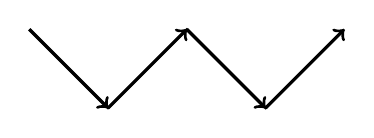
\begin{tikzpicture}
		% define point
		\coordinate (A)  at (1, 1);
		\coordinate (O)  at (2, 0);
		\coordinate (B)  at (3, 1);
		\coordinate (C)  at  (4,0);
		\coordinate (D) at  (5,1);
		% angle  
		\draw[thick] (A) -- (O) -- (B) -- (C)-- (D);
		%	\draw pic[draw=black,eccentricity=2.9]
		%\pic [draw,"$\alpha_1$",angle radius=20,->,angle eccentricity=1.4]
		%  {angle = B--O--A};
		\draw [->, very thick] (1,1) -- (2,0)  node [midway, above] {\scriptsize };
		\draw [->, very thick] (2,0) -- (3,1)  node [midway, above] {\scriptsize };
		\draw [->, very thick] (3,1) -- (4,0)  node [midway, above] {\scriptsize };
		\draw [->, very thick] (4,0) -- (5,1)  node [midway, above] {\scriptsize };
	\end{tikzpicture}
	\captionof{figure}{\textbf{Wing Gesture \cite{War:2020}}}
\end{center}
\begin{itemize}
	\item The device is first moved down and to the right.
	\item Then the device is moved up and to the right.
	\item The device is then moved down and to the right.
	\item The device is then moved up and to the right again. 
	
\end{itemize}

	Shows a sample of real data captured during the ``wing'' gesture, measured in milli-Gs.  

	The process involved in capturing a ring is as follows. \cite{War:2020}

\begin{center}
	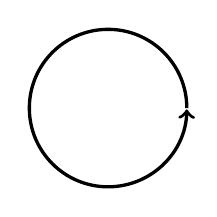
\begin{tikzpicture}
		\draw[->,very thick] (0,0) arc[radius=1cm,start angle=0,delta angle=359];
	\end{tikzpicture}
	\captionof{figure}{\textbf{Ring Gesture \cite{War:2020}}}
\end{center}

\begin{itemize}
	\item Trace a clockwise circle using the wand.
	
	\item Aim again to take around a second to perform the gesture.
	
\end{itemize}

	The steps involved in waving the slope gesture are mentioned below \cite{War:2020}:

\begin{center}
	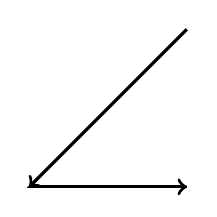
\begin{tikzpicture}
		% define point
		\coordinate (A)  at (2, 2);
		\coordinate (O)  at (0, 0);
		\coordinate (B)  at (2, 0);
		% angle  
		\draw[thick] (A) -- (O) -- (B);
		%\draw pic[draw=black,angle radius=20,angle eccentricity=1.4]
		%{angle = B--O--A};
		%\pic [draw,"$\alpha_1$",angle radius=20,->,angle eccentricity=1.4]
		%  {angle = B--O--A};
		\draw [->, very thick] (2,2) -- (0,0)  node [midway, above] {\scriptsize };
		\draw [->, very thick] (0,0) -- (2,0)  node [midway, above] {\scriptsize };
	\end{tikzpicture}
	\captionof{figure}{\textbf{Slope Gesture \cite{War:2020}}}
\end{center}

\begin{itemize}
	\item The device is first moved down and to the left.
	\item Then the device is moved to the right.
	\item Finally you should get a corner of the triangle as shown in the figure.
\end{itemize}

	The process is repeated until around 15 readings are captured by the wand for Data Preparation and Transformation. 

	In order to consider the unknown readings, we will be carrying out another set of procedures to feed with unknown data. This would help the wand recognize any unknown gesture and give the output that it is false. \cite{War:2020}

	All readings are recorded in a unique text file for each gesture. The files \FILE{.txt} \cite{DataPrep:21} contain raw accelerometer data that would later be transformed into machine learning language that should be interpreted by the compiler. \cite{War:2020}

	Since no existing databases exist for the model, a new database will be created.The database is a .txt file which contains raw data from the accelerometer readings recognized by the board Arduino Nano 33 BLE Sense. Since the way a person records the gesture varies from one to another, the gestures of three people are recorded as we are a group of three members. In order to the database to have a vast amount of data, each person will record at least 50 trials for each gesture. In order for the database to be more accurate data from both hands of the three users were used. This would improve the efficiency and effectiveness of the database making it more concrete. It is also possible to add further data to our model, improving it over time. The size of the database thus created will be petite, less than 2 MB. Obtaining sufficient data is one of the major concerns in a machine learning project and the amount of data involved in our data set is very small. The data thus created will be further used in the next step “Data Preparation and Transformation” where this raw data is further processed and the outliers are identified and removed if necessary.

\section{Data Quantity} 
\subsubsection{Edge Computing}
	The placement of computer and storage resources at the point where data produced is known as edge computing. This computes and stores  the data source at the network edge, which is optimal. In other words, instead of sending raw data to a main data centre for processing and analysis, this work is done right where the data is generated.
	Edge computing is used to handle discrete tasks like determining if someone answered "yes" and responding appropriately. Instead of comparing the data with that on the web, the audio analysis is done on the edge. This drastically decreases expenses and complexity while also reducing the risk of data breaches.\cite{Big:2021}

	Edge computing has gained traction as a viable solution to a variety of issues related to transporting the massive amounts of data that today's businesses generate and consume. It's not just a matter of quantity, it's also a matter of time; applications increasingly rely on processing and responses that are time-sensitive.The analysis and analysis of data produced by connected devices is made possible by edge computing, a crucial element of the Internet of Things (IoT).\cite{Haz:2021} claims that edge computing enables data collecting, processing, and analysis at the network’s edge, facilitating in-the-moment decision-making and minimizing the need to send data to a central point for processing. Edge computing reduces processing times for data, allowing businesses to react swiftly to shifting operational circumstances.

\section{Data Quality}
	Creating a magic wand with board Arduino Nano 33 BLE Sense involves integrating various sensors components and programming logic to ensure data quality for a successful project you need to consider the reliability and accuracy of the data collected from sensors here are some key considerations\cite{Daity:21}.
\subsubsection{Sensor Calibration}
	Sensor calibration calibrate sensors such as accelerometers gyroscopes or magnetometers to ensure accurate readings understand the sensor s specifications and calibrate them accordingly to reduce errors in measurements
\subsubsection{Sensor Fusion}
	Sensor fusion use sensor fusion techniques to combine data from multiple sensors this can improve the accuracy and reliability of the data implement sensor fusion algorithms to obtain a more comprehensive understanding of the wand s orientation and movement
\subsubsection{Wireless Communication Reliability}
	Wireless communication reliability if your magic wand involves wireless communication ensure the bluetooth low energy ble connection is stable and reliable implement error checking mechanisms to handle potential data transmission issues \cite{Gomez:2012}
\subsubsection{Code Optimization}
	Write efficient and optimized code to minimize delays and improve the real-time response of the magic wand.
	Optimize algorithms to reduce processing time and enhance overall system performance.




\section{Data Relevance}
\subsubsection{Real-Time Machine Learning}
	Real Time can be considered as a way of training the model by making it run through live data constantly in order to improve the model. This contradicts the traditional way of machine learning when machine learning engineers were dependent already existent data inputs for creating the model. A method by which we can implement real time learning in to a machine learning model is by continuously feeding it with a data stream and improving the model over time. This is achieved by using an event driven architecture. Event driven architecture is a modern design and development approach that centers about the events occurring in the model. Event-driven architectures create, detect, consume, and react to events.\cite{Haz:2021}. By using a scalable event driven architecture, large number of events in real time can be responded, to which are suitable for loosely coupled softwares(For eg: web services). They also work well with unpredictable and non linear events by making it versatile. \cite{Haz:2021}



\section{Outliers}
	Outliers refer to exceptional or irregular data points that deviate significantly from the expected sensor readings or user interactions. These anomalies can arise from various sources such as sudden movements, extreme sensor values, interference, or unexpected user inputs.outliers in sensor data might occur if the accelerometer or gyroscope registers an unusually rapid or erratic movement that does not align with typical usage patterns. Similarly, outliers in user interaction may manifest as unintended button presses or variations in touch sensor sensitivity.

	Detecting and handling outliers is crucial for ensuring the accuracy and reliability of the magic wand's functionality. Strategies may involve implementing filtering algorithms, calibration techniques, and debouncing mechanisms to mitigate the impact of outliers on sensor readings and user inputs.\cite{Munoz:2019}
\section{Anomalies}
	Creating a magic wand with Arduino Nano 33 BLE involves considering potential anomalies or unexpected behaviors that might arise during the development and usage of the wand. The major challenge while preparing data can be the presence of outliers or anomalies where there are unexpected values. This can be overcome by feeding our model with more data so that the model is efficient.\cite{War:2020}
\begin{itemize}
\subsubsection{Sensor Anomalies}

	\item Accelerometer/Gyroscope Drift
	- Sensors like accelerometers and gyroscopes may experience drift over time, leading to inaccuracies in orientation tracking. Calibration techniques can help mitigate this issue.\cite{Chow:2021}
	\item {Magnetic Interference}
	- Magnetometers can be affected by nearby magnetic fields, leading to anomalies in readings. Shielding or compensation algorithms may be required.
\subsubsection{Power Anomalies}
	\item Unexpected Power Drain
	- Identify and address any unexpected power consumption patterns. Implement power-efficient code and periodically monitor power usage to detect anomalies.
	\item Battery Voltage Fluctuations
	- Voltage fluctuations in the power supply can affect the stability of the Arduino Nano 33 BLE. Implement voltage regulation and monitoring to handle such anomalies. 
\subsubsection{Firmware and Software Anomalies}
	\item Memory Issues
	- Anomalies may occur due to memory limitations on the Arduino Nano 33 BLE. Monitor and optimize memory usage to avoid crashes or unexpected behavior.
	\item Firmware Bugs
	-  Identify and address potential bugs in your firmware. Regular testing, debugging, and code reviews can help mitigate software anomalies.
\end{itemize}

%%%%%%
%%%%%%%%%%%%%%%%%%%%%%%%
%
% $Author: Adhiraj Walse $
% $Datum: 2023-10-31  $
%$Pfad:Users/Documents/ML23-06-Magic-Wand-with-an-Arduino-Nano-33-BLE-sense/report/Contents/en/HardwareDescription.tex $
% $Version: 1.0 $
%
% $Short Description: Describe hardware that we use in our Magic Wand Project and testing on the hardware$
%%%%%%%%%%%%%%%%%%%%%%%%


\chapter{Hardware Description}
\label{chapter 3}

\section{Board Arduino Nano 33 BLE Sense}

The Arduino Nano 33 BLE Sense board serves as a prime example of edge computing. It integrates multiple sensors alongside BLE connectivity and wireless communication features \cite{Raj:2019}, making it suitable for a wide range of IoT and wearable applications. Equipped with sensors for temperature, pressure, magnetometry, acceleration, and gyroscopic measurements \cite{Raj:2019}, the board also includes a microphone and a proximity sensor. Its built-in BLE capabilities enable seamless interaction with other BLE-compatible devices, such as smartphones, facilitating remote data collection and control \cite{Bagur:2023}. At Magic Wand, our focus lies in leveraging the Accelerometer, Gyroscope, and Magnetometer sensors. The Arduino Nano 33 BLE Sense stands out as a versatile board, ideal for applications requiring sensor integration and wireless communication in IoT and wearable technologies \cite{Raj:2019}.

The Arduino Nano 33 BLE Sense is a compact, microcontroller-based development board designed to operate at a maximum of 3.3V. It is essential to avoid exceeding this voltage on its digital and analog pins \cite{Arduino:2021}. The board features a Bluetooth Low Energy (BLE) module, making it suitable for IoT applications \cite{Bagur:2023}. Powered by an nRF52840 processor, it boasts a 64 MHz clock speed, 256 KB of SRAM, and 1 MB of flash memory. Additionally, it includes 14 digital I/O pins, eight of which are analog input pins for connecting external components and sensors. The board’s power consumption is remarkably low, drawing only 10 mA per I/O pin \cite{Arduino:2021}.  

The Arduino Nano 33 BLE Sense supports high-level programming languages similar to C/C++ \cite{Emeritus:2023}. Programming for microcontrollers, including Arduino, is done on a host computer. Code is written and compiled using Arduino’s Integrated Development Environment (IDE) before being uploaded to the microcontroller for execution. To connect the board, a micro-USB cable is used, linking the board to a laptop. Once powered, a green LED next to the micro-USB port indicates a successful connection.

Additionally, Arduino offers several versions of the Nano 33 BLE board. This includes the Nano 33 BLE Sense and Nano 33 BLE Sense Lite. The Lite version lacks the HTS221 temperature and humidity sensor, instead featuring the LPS22HB pressure sensor, which can measure temperature but not humidity \cite{Arduino:2022}. Since our project focuses on the IMU sensor for gesture recognition, both versions are suitable for use. The following descriptions and hardware tests are based primarily on the Arduino Nano 33 BLE Sense.

\begin{figure}[h!]
	\includegraphics[width=\linewidth]{Images/HardwareDescription/ArduinoTop}
	\caption{\textbf{Top View of Board Arduino Nano 33 BLE Sense}}
	\label{fig:Top View of Board Arduino Nano 33 BLE Sense}
	\cite{Arduino:2023}
\end{figure}

\begin{figure}[h!]
	\includegraphics[width=\linewidth]{Images/HardwareDescription/ArduinoBottom}
	\caption{\textbf{Bottom View of Board Arduino Nano 33 BLE Sense}}
	\label{fig:Bottom View of Board Arduino Nano 33 BLE Sense} \cite{Arduino:2023}
\end{figure}


\section{Interfaces}

\subsection{Board Arduino Nano 33 BLE Sense: Components Overview}\label{BoardDescription}



The Arduino Nano 33 BLE Sense is equipped with several embedded sensors, including humidity, temperature, barometric pressure, proximity, and a microphone. These built-in components allow the board to be utilized for various practical applications without the need for additional circuitry \cite{Arduino:2021}. It supports standard communication protocols such as UART, I2C, and SPI, enabling seamless interaction with external circuits and sensors for data exchange. The board includes a micro-USB port for connecting to a laptop or desktop, which serves as both a power supply and a medium for file or data transfer via serial communication. While operating the board, it is crucial to ensure that no more than 3.3V is applied to its pins, as exceeding this voltage can result in permanent damage \cite{Arduino:2021}.

Below is a detailed description of each sensor embedded on the board:

\begin{center}
	\begin{tikzpicture}
		\ArduinoNanoTikz
		
		\node(HTS) at (-10,5){\textcolor{red}{\tiny HTS221}};
		\draw[line width=1pt,red]  (-6.3,2.8) -- (-10,4.9);
		\node(APD) at (-6,5){\textcolor{red}{\tiny APDS9960}};
		\draw[line width=1pt,red]  (-5,2.25) -- (-6,4.9);
		\node(LSM9DS1) at (-2,5){\textcolor{red}{\tiny LSM9DS1}};
		\draw[line width=1pt,red]  (-5,3.15) -- (-2,4.9);
		
		\node(LSM9DS1) at (1,5){\textcolor{red}{\tiny RGB Programmable LED}};
		\draw[line width=1pt,red]  (-3.6,2.95) -- (1,4.9);
		
		\node(HTS) at (1.5,2.25){\textcolor{red}{\tiny Nordic nRF 52840}};
		\draw[line width=1pt,red]  (-2,2.25) -- (0.5,2.25);
		
		\node(MP) at (-2,-0.75){\textcolor{red}{\tiny MP34DT05-A}};
		\draw[line width=1pt,red]  (-3.9,2.25) -- (-1.75,-0.6);
		
		\node(MP) at (-6,-0.75){\textcolor{red}{\tiny LPS22HB}};
		\draw[line width=1pt,red]  (-4.5,1.0) -- (-6,-0.6);
		
		\node(LEDPower) at (-11.5,3.55){\textcolor{red}{\tiny Power LED}};
		\draw[line width=1pt,red]  (-10.8,3.55) -- (-10,3.55);
		
		\node(USB) at (-12,2.25){\textcolor{red}{\tiny Micro-USB Port}};
		\draw[line width=1pt,red]  (-11.1,2.25) -- (-10.2,2.25);
		
		\node(LEDOrange) at (-11.8,0.8){\textcolor{red}{\tiny Progammable LED}};
		\draw[line width=1pt,red]  (-10.8,0.8) -- (-10,0.8);
		
	\end{tikzpicture}
	\captionof{figure}{}\label{ArduinoNano33BLESenseArchitecture}
\end{center}

\begin{itemize}
	\item LSM9DS1 - \ac{imu} features a 3D accelerometer, gyroscope and magnetometer and allows you to detect orientation, motion or vibrations in your project \cite{Alushi:2023}.
	\item  APDS-9960 - The APDS-9960 chip allows for measuring digital proximity and ambient light as well as for detecting RGB colors and gestures \cite{Avago:2015}.
	\item  LPS22HB - The LPS22HB picks up on barometric pressure and allows for a 24-bit pressure data output between 260 and 1260 hPa. This data can also be processed to calculate the height above sea level of the current location \cite{Stm:2017}.
	\item HTS221 - The HTS221 capacitive digital sensor measures relative humidity and temperature. It has a temperature accuracy of ± 0.5 °C (between 15-40 °C) and is perfectly suited to detect ambient temperature \cite{Stm:2023}.
	\item MP34DT05 - The MP34DT05 microphone allows you to capture and analyze sound in real-time and can be used to create a voice interface for your project\cite{Stm:2021}.
	\item USB port - USB port allows you to connect Arduino Nano 33 BLE sense to your machine.
	\item LEDs - There are 3 different LEDs that can be accessed on the Nano BLE Sense: \ac{rgb}(Programmable LED), the built-in LED(Programmable LED) and the power LED
\end{itemize}

\subsubsection{LEDs function in Board Arduino Nano 33 BLE Sense}
Apart from the Power LED indicate the board is powered, there are two LEDs in the board: Programmable LED(orange) and the RGB Programmable LED. The orange LED sparkles when it is connected to the computer. The RGB LED can be used during the creation of the actions that we perform. For example, in our project, each gesture can use one color to represent a specific gesture, indicating as the recognizing function. 

\section{Arduino Nano 33 BLE Pin Configuration}

The \textbf{Arduino Nano 33 BLE} is an advanced version of the Arduino Nano board that is based on a powerful processor, the nRF52840. The following is the pin configuration of the board:

\subsection{Pin Configuration}
\textbf{Digital Pins:}
\begin{itemize}[noitemsep]
	\item The board has \textbf{14 digital I/O pins} that receive only two values: HIGH or LOW.
	\item These pins can function as input or output based on the requirement.
	\item When the pins receive 5V, they are in a HIGH state; when they receive 0V, they are in a LOW state.
\end{itemize}

\textbf{Analog Pins:}
\begin{itemize}[noitemsep]
	\item The board has a total of \textbf{8 analog pins} (A0–A7).
	\item These pins measure analog voltage ranging between 0 to 5V and can get any value as opposed to digital pins, which only receive HIGH or LOW values.
\end{itemize}

\textbf{PWM Pins:}
\begin{itemize}[noitemsep]
	\item All digital pins can be used as PWM pins.
	\item These pins generate analog results using digital means.
\end{itemize}

\textbf{SPI Pins:}
\begin{itemize}[noitemsep]
	\item The board supports the \textbf{Serial Peripheral Interface (SPI)} communication protocol.
	\item SPI is used to communicate between the controller and peripheral devices such as shift registers and sensors.
	\item Two pins, \textbf{MISO} (Master Input Slave Output) and \textbf{MOSI} (Master Output Slave Input), are used for SPI communication.
\end{itemize}

\textbf{I2C Pins:}
\begin{itemize}[noitemsep]
	\item The board supports the \textbf{I2C communication protocol}, a two-wire protocol.
	\item It includes two pins: \textbf{SDL} and \textbf{SCL}.
\end{itemize}

\textbf{UART Pins:}
\begin{itemize}[noitemsep]
	\item The board features the \textbf{UART communication protocol} for serial communication.
	\item It includes two pins: \textbf{Rx} (receiving pin) and \textbf{Tx} (transmitting pin).
\end{itemize}

\textbf{External Interrupts Pins:}
\begin{itemize}[noitemsep]
	\item All digital pins can be used as external interrupt pins.
	\item This feature allows the main running program to be interrupted and handle emergency instructions.
\end{itemize}

\textbf{LED at Pin 13 and AREF Pin:}
\begin{itemize}[noitemsep]
	\item There is an \textbf{LED connected to pin 13} of the board.
	\item The \textbf{AREF pin} is used as a reference voltage for input voltage.
\end{itemize}

\begin{figure}[h!]
	\includegraphics[width=\linewidth]{Images/HardwareDescription/Pin_Configuration}
	\caption{\textbf{Arduino Nano 33 BLE Pin Configuration}}
	\label{Arduino Nano 33 BLE Pin Configuration} \cite{Arduino:2023}
\end{figure}

\section{Data Quality in Hardware Description}

In the hardware description of our Magic Wand project with Arduino Nano 33 BLE Sense, we consider the following aspects related to data quality:

\begin{enumerate}
	\item \textbf{Sensor Accuracy:} The sensors embedded in the Arduino Nano 33 BLE Sense board deliver precise measurements of environmental parameters such as motion, orientation, temperature, humidity, and pressure \cite{Dhow:2024}.
	
	\item \textbf{Resolution:} Each sensor has a defined resolution, representing the smallest detectable input change. For instance, the accelerometer’s resolution is \textless{}insert value\textgreater{}, allowing detection of subtle motion variations.
	
	\item \textbf{Sampling Rate:}The board supports high sampling rates, enabling real-time data acquisition at \textless{}insert frequency\textgreater{} Hz. This is essential for applications requiring continuous and responsive data collection.
	
	\item \textbf{Noise Level:} Sensor data may exhibit noise due to factors such as environmental conditions, sensor imperfections, or electromagnetic interference. The board minimizes noise using calibration and filtering techniques, ensuring high data fidelity.
	
	\item \textbf{Calibration:} Calibration processes are applied to enhance the accuracy and reliability of sensor readings. These procedures involve fine-tuning sensor settings and using correction factors to address systematic errors \cite{Edm:2015}.
	
	\item \textbf{Data Transmission:} Sensor data is transmitted from the Arduino Nano 33 BLE Sense board to other devices using wireless communication protocols such as Bluetooth Low Energy (BLE). Data transmission is efficient, ensuring minimal latency and reliable delivery.
	
	\item \textbf{Data Integrity:} To maintain data integrity during transmission and processing, error detection and correction mechanisms are implemented. These measures help identify and resolve issues like data loss or corruption \cite{TensorFlow:2023}.
	
	\item \textbf{Power Consumption:} The Arduino Nano 33 BLE Sense is designed for low power consumption, making it ideal for battery-powered applications. Its optimized power management extends battery life without compromising continuous data collection.
\end{enumerate}

By addressing these aspects of data quality in the hardware description, we ensure the reliability and accuracy of sensor data used in our Magic Wand project.
\begin{center}
	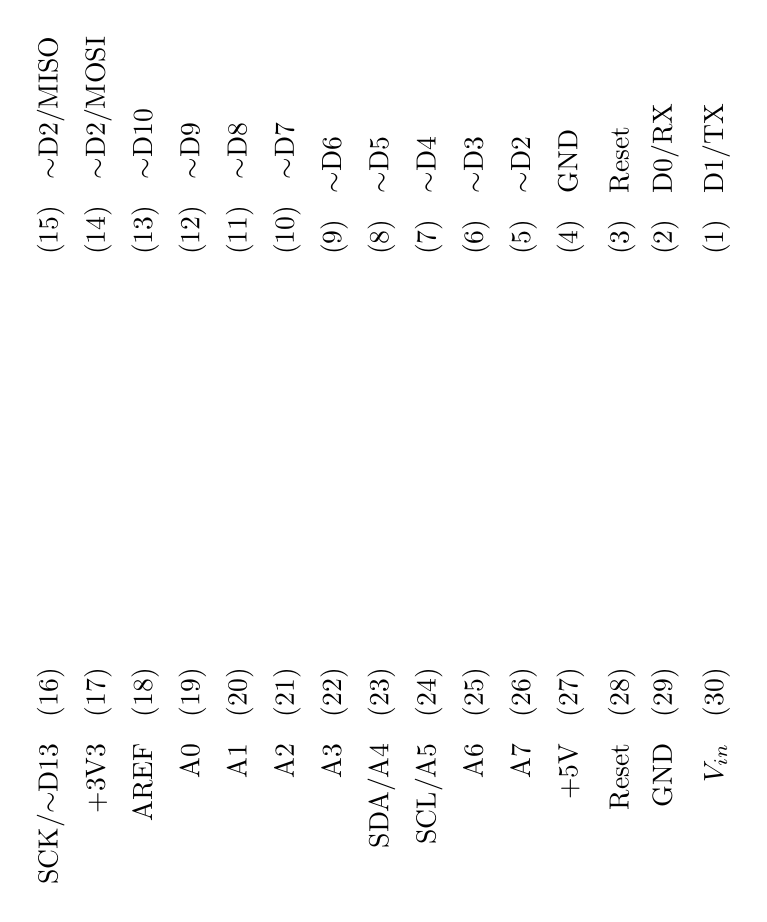
\begin{tikzpicture}
		
		\ArduinoNanoTikz
		
		\node[rotate=90,right] (Pin1) at (-0.91,4.6) {(1) \; D1/TX};
		\node[rotate=90,right] (Pin2) at (-1.56,4.6) {(2) \; D0/RX};
		\node[rotate=90,right] (Pin3) at (-2.11,4.6) {(3) \; Reset};
		\node[rotate=90,right] (Pin4) at (-2.76,4.6) {(4) \; GND};
		\node[rotate=90,right] (Pin5) at (-3.36,4.6) {(5) \; $\sim$D2};
		\node[rotate=90,right] (Pin6) at (-3.96,4.6) {(6) \; $\sim$D3};
		\node[rotate=90,right] (Pin7) at (-4.56,4.6) {(7) \; $\sim$D4};
		\node[rotate=90,right] (Pin8) at (-5.16,4.6) {(8) \; $\sim$D5};
		\node[rotate=90,right] (Pin9) at (-5.76,4.6) {(9) \; $\sim$D6};
		\node[rotate=90,right] (Pin10) at (-6.36,4.6) {(10) \; $\sim$D7};
		\node[rotate=90,right] (Pin11) at (-6.96,4.6) {(11) \; $\sim$D8};
		\node[rotate=90,right] (Pin12) at (-7.56,4.6) {(12) \; $\sim$D9};
		\node[rotate=90,right] (Pin13) at (-8.16,4.6) {(13) \; $\sim$D10};
		\node[rotate=90,right] (Pin14) at (-8.76,4.6) {(14) \; $\sim$D2/MOSI};
		\node[rotate=90,right] (Pin15) at (-9.36,4.6) {(15) \; $\sim$D2/MISO};
		
		
		\node[rotate=90,left] (Pin30) at (-0.91,-0.4) { $V_{in}$ \; (30)};
		\node[rotate=90,left] (Pin1) at (-1.56,-0.4) {GND \; (29)};
		\node[rotate=90,left] (Pin2) at (-2.11,-0.4) {Reset \; (28)};
		\node[rotate=90,left] (Pin3) at (-2.76,-0.4) {+5V \; (27)};
		\node[rotate=90,left] (Pin4) at (-3.36,-0.4) {A7 \; (26)};
		\node[rotate=90,left] (Pin5) at (-3.96,-0.4) {A6 \; (25)};
		\node[rotate=90,left] (Pin6) at (-4.56,-0.4) {SCL/A5 \; (24)};
		\node[rotate=90,left] (Pin7) at (-5.16,-0.4) {SDA/A4 \; (23)};
		\node[rotate=90,left] (Pin8) at (-5.76,-0.4) {A3 \; (22)};
		\node[rotate=90,left] (Pin9) at (-6.36,-0.4) {A2 \; (21)};
		\node[rotate=90,left] (Pin10) at (-6.96,-0.4) {A1 \; (20)};
		\node[rotate=90,left] (Pin11) at (-7.56,-0.4) {A0 \; (19)};
		\node[rotate=90,left] (Pin12) at (-8.16,-0.4) {AREF \; (18)};
		\node[rotate=90,left] (Pin13) at (-8.76,-0.4) {+3V3 \; (17)};
		\node[rotate=90,left] (Pin14) at (-9.36,-0.4) {SCK/$\sim$D13 \; (16)};
		
	\end{tikzpicture}
	\captionof{figure}[Pin assignment of the Arduino Nano 33 BLE Sense]{Pin assignment of the Arduino Nano 33 BLE Sense; note that the orange built-in LED is connected to pin D13 and the power LED to pin D1. The built-in RGB LED occupies pins D18, D19 and D20.}
\end{center}

\subsection{Specifications of Arduino Nano 33 BLE Sense}


\subsubsection*{NINA B306 Module}
\begin{enumerate}[label=\arabic*.]
	\item Processor:
	\begin{itemize}[label=-]
		\item 64 MHz Arm® Cortex-M4F (with FPU)
		\item 1 MB Flash + 256 KB RAM
	\end{itemize}
	\item Bluetooth® 5 multiprotocol radio:
	\begin{itemize}[label=-]
		\item 2 Mbps
		\item +8 dBm TX power
		\item -95 dBm sensitivity
		\item 4.8 mA in TX (0 dBm)
		\item 4.6 mA in RX (1 Mbps)
		\item Integrated balun with 50 Ohm single-ended output
		\item IEEE 802.15.4 radio support
	\end{itemize}
	\item Peripherals:
	\begin{itemize}[label=-]
		\item 12 Mbps USB
		\item NFC-A tag
		\item Arm CryptoCell CC310 security subsystem
		\item QSPI/SPI/TWI/I2S/PDM/QDEC
		\item 32 MHz SPI
		\item Quad SPI interface 32 MHz
		\item 12-bit 200 ksps ADC
		\item 128 bit AES/ECB/CCM/AAR co-processor
	\end{itemize}
\end{enumerate}

\subsubsection*{LSM9DS1 (9 axis IMU)}\cite{Warden:2020}
\begin{enumerate}[label=\arabic*.]
	\item 3 acceleration channels, 3 angular rate channels, 3 magnetic field channels
	\item $\pm$2/$\pm$4/$\pm$8/$\pm$16 g linear acceleration full scale
	\item $\pm$4/$\pm$8/$\pm$12/$\pm$16 gauss magnetic full scale
	\item $\pm$245/$\pm$500/$\pm$2000 dps angular rate full scale
	\item 16-bit data output
\end{enumerate}




\section{Data quantity in Hardware Description}

\begin{enumerate}
	\item \textbf{Sensor Data}: The Arduino Nano 33 BLE Sense board is equipped with a variety of sensors, including an accelerometer, a gyroscope, and a magnetometer. These sensors generate a large amount of data as you wave the magic wand. For instance, in one experiment, a window size of 2 seconds was used, which means 200 rows of accelerometer data or 600 values of x, y, and z acceleration axis were fed into the model. \cite{Miller:2022}
	
	\item \textbf{Data Processing Capacity}: The Arduino Nano 33 BLE Sense board has a 32-bit ARM Cortex-M4 CPU running at 64 MHz, which allows it to process a significant amount of sensor data in real-time.
	
	\item \textbf{Memory}: The board has 1MB of flash memory and 256KB of SRAM. This memory is used to store the program code and handle runtime operations, including storing sensor data and machine learning model parameters.
	
	\item \textbf{Machine Learning Model}: The size of the machine learning model used in the project also affects the quantity of data. The model needs to be small enough to fit into the board's memory along with the program code.
	
	\item \textbf{Data Transmission}: The board also has a built-in Bluetooth Low Energy module, which can be used to transmit sensor data to another device for further processing. \cite{TensorFlow:2023}
	
\end{enumerate}


\section{Constraints}
\subsubsection{Arduino Nano 33 BLE Sense}
\begin{itemize}[label=--]
	\item Operating Voltage: 3.3V
	\item Power Consumption:
	\begin{itemize}[label=--,leftmargin=*]
		\item Maximum 15mA in low power mode
		\item Maximum 60mA in active mode
	\end{itemize}
	\item Operating Temperature Range: -40°C to 85°C
	\item Memory Constraints: 1 MB Flash + 256 KB RAM
	\item Communication Interfaces: USB, Bluetooth 5, NFC-A, SPI, I2C, QSPI, etc.\cite{Arduino:2015}
\end{itemize}

\subsubsection*{Sensors}
\begin{itemize}[label=--]
	\item Accelerometer:
	\begin{itemize}[label=--,leftmargin=*]
		\item Measurement Range: ±8g
		\item Operating Temperature Range: -40°C to 85°C
	\end{itemize}
	\item Gyroscope:
	\begin{itemize}[label=--,leftmargin=*]
		\item Measurement Range: ±2000 dps
		\item Operating Temperature Range: -40°C to 85°C \cite{Arduino:2021}
	\end{itemize}
	
\end{itemize}


\subsubsection*{Actuators}
\begin{itemize}[label=--]
	\item RGB LEDs:
	\begin{itemize}[label=--,leftmargin=*]
		\item Power Requirements: Voltage, Current
		\item Operating Temperature Range
	\end{itemize}
	\item Buzzer/Speaker:
	\begin{itemize}[label=--,leftmargin=*]
		\item  Voltage, Current, Sound Output Levels
	\end{itemize}
	
\end{itemize}

\subsubsection*{Power Supply}
\begin{itemize}[label=--]
	\item Input Voltage Range: Specify the acceptable input voltage range.
	\item Power Consumption: Estimate the overall power consumption of the system.
\end{itemize}

\subsubsection*{Physical Constraints}
\begin{itemize}[label=--]
	\item Size and Dimensions: Ensure compatibility with the project enclosure or housing.
	\item Mounting Requirements: Specify any specific mounting requirements for the components.
\end{itemize}

\subsubsection*{Environmental Constraints}
\begin{itemize}[label=--]
	\item Environmental Protection: Ensure components are suitable for the intended environmental conditions (e.g., moisture resistance, dust resistance).
	\item Operating Conditions: Specify any limitations or special considerations for operating in certain environments.\cite{Arduino:2021}
\end{itemize}



\section{Dimensions of the Arduino Nano 33 BLE Sense}



The Arduino Nano 33 BLE Sense is a highly compact development board, measuring just 45mm x 18mm. Its small form factor makes it particularly well-suited for wearable devices and other space-constrained applications. Despite its size, the board is equipped with a wide range of sensors and features, offering versatility for various projects.

It is important to note that these dimensions apply to the board without headers. If you are using a version with pre-soldered headers or attaching additional components, the overall dimensions of your hardware setup may change. For precise measurements, always consult the specifications of your specific board and components \cite{Arduino:2023}.


\section{Sensor Accelerometer, Gyroscope, and Magnetometer LSM9DS1}\label{boardsensor}

Magic Wand gesture detection is mainly based on the sensor LSM9DS1 at the board. It is a system-in-package featuring a 3D digital linear acceleration sensor, a 3D digital angular rate sensor, and a 3D digital magnetic sensor. A tiny device called an Inertial Measurement Unit (IMU) in the sensor is used to detect the motions physically \cite{Alushi:2023}. It has several components, including magnetometer, gyroscope, and accelerometer. By monitoring  acceleration and angular velocity changes, the IMU sensor is critical for identifying an object's orientation and movement in real-time \cite{Alushi:2023}.





\subsection*{Example Code for Arduino Nano 33 BLE Sense}
Below is a simple example demonstrating how to use the built-in microphone on the Arduino Nano 33 BLE Sense:

\begin{code}
	\begin{Arduino}
		// Include the PDM library
		#include <PDM.h>
		
		// Buffer to store the microphone data
		short sampleBuffer[256];
		
		// Variable to store the sound level
		int soundLevel = 0;
		
		// Callback function for PDM data
		void onPDMdata() {
			// Read the PDM data
			int bytesAvailable = PDM.available();
			PDM.read(sampleBuffer, bytesAvailable);
			
			// Calculate the sound level
			soundLevel = 0;
			for (int i = 0; i < bytesAvailable / 2; i++) {
				soundLevel += abs(sampleBuffer[i]);
			}
			soundLevel /= bytesAvailable / 2;
		}
		
		void setup() {
			// Initialize serial communication
			Serial.begin(9600);
			while (!Serial);
			
			// Initialize PDM with a sample rate of 16 kHz and 16-bit resolution
			PDM.begin(1, 16000);
			PDM.onReceive(onPDMdata);
		}
		
		void loop() {
			// Print the sound level to the serial monitor
			Serial.println(soundLevel);
			delay(100);
		}
	\end{Arduino}
	\caption{Simple example using of the builtin microphone of the Arduino Nano 33 BLE Sense}\label{code:microphone}
\end{code}

\begin{code}
	\begin{Arduino}
		// Include the ArduinoBLE library
		#include <ArduinoBLE.h>
		
		// Create a BLE service
		BLEService batteryService("1101");
		
		// Create a BLE characteristic
		BLEUnsignedCharCharacteristic batteryLevelChar("2101", BLERead | BLENotify);
		
		void setup() {
			// Initialize serial communication
			Serial.begin(9600);
			while (!Serial);
			
			// Set up the built-in LED pin
			pinMode(LED_BUILTIN, OUTPUT);
			
			// Initialize BLE
			if (!BLE.begin()) {
				Serial.println("Starting BLE failed!");
				while (1);
			}
			
			// Set the BLE local name and advertised service
			BLE.setLocalName("BatteryMonitor");
			BLE.setAdvertisedService(batteryService);
			
			// Add characteristic to the service
			batteryService.addCharacteristic(batteryLevelChar);
			
			// Add the service and start advertising
			BLE.addService(batteryService);
			BLE.advertise();
			
			Serial.println("Bluetooth device active, waiting for connections...");
		}
		
		void loop() {
			// Wait for a BLE central to connect
			BLEDevice central = BLE.central();
			
			if (central) {
				Serial.print("Connected to central: ");
				Serial.println(central.address());
				
				// Turn on the built-in LED
				digitalWrite(LED_BUILTIN, HIGH);
				
				// Loop while the central device is connected
				while (central.connected()) {
					int battery = analogRead(A0);
					int batteryLevel = map(battery, 0, 1023, 0, 100);
					
					Serial.print("Battery Level is now: ");
					Serial.println(batteryLevel);
					
					// Update the characteristic value
					batteryLevelChar.writeValue(batteryLevel);
					
					delay(200);
				}
				
				// Turn off the built-in LED
				digitalWrite(LED_BUILTIN, LOW);
				Serial.print("Disconnected from central: ");
				Serial.println(central.address());
			}
		}
	\end{Arduino}
	\caption{Example of a BLE Battery Monitor using Arduino Nano 33 BLE Sense}\label{code:battery-monitor}
\end{code}

\pagebreak
\section{Inertial Measurement Unit (IMU)}\label{IMU}

\subsection{Description}
An Inertial Measurement Unit (IMU) is an electronic system that measures movement across multiple axes using three primary sensors: an accelerometer, a gyroscope, and a magnetometer.\cite{Qureshi:2017} These sensors work together to provide data on acceleration, rotational motion, and magnetic fields, making IMUs essential for a wide range of applications such as navigation, fitness tracking, and robotics.\cite{Qureshi:2017}

{General}
IMUs have become increasingly common in microcontroller projects, with some boards, such as the Arduino Nano 33 BLE Sense, featuring integrated IMUs for seamless development of motion-sensitive applications.\cite{Zhou:2020}

\subsection{Specific Sensors}
\textbf{Continuous Operation ("Always-On" Mode)}
The LSM9DS1 supports an "Always-On" mode, ensuring continuous operation even when the main system is in a low-power state.\cite{Zhou:2020} This is critical for uninterrupted motion monitoring in devices like the Magic Wand, where gestures must be tracked instantly. With a power consumption of just 0.55 mA in high-performance mode, it provides precise and reliable motion data while preserving battery life.\cite{Zhou:2020}

\textbf{Tilt Detection}
Using the accelerometer, the IMU can detect orientation changes with minimal power usage. Tilt detection is particularly useful for identifying subtle shifts in position, enhancing the responsiveness of gesture-based controls.\cite{Zhou:2020}

\textbf{Significant Motion Detection}
The accelerometer enables significant motion detection (SMD), which recognizes large-scale movements. SMD can be used to activate specific device functions, such as waking the system from sleep mode or triggering predefined actions based on significant gestures.\cite{Zhou:2020}

The LSM9DS1 is a versatile and energy-efficient IMU with advanced sensing capabilities, supporting a range of applications where motion detection, orientation tracking, and gesture recognition are essential. Its compact design, low power consumption, and robust environmental tolerance make it a reliable choice for portable, battery-powered devices like the Magic Wand.\cite{Zhou:2020}

An \ac{imu} consists of three sensors that measure an object's orientation, position, vibration and movement in 3D space in real-time. These sensors are typically arranged in a pattern, including a tri-axial accelerometer, gyroscope, and magnetometer\cite{Ahmad:2013}. An accelerometer is used to measure the change in velocity of a moving or vibrating object\cite{Ahmad:2013}. Gyroscope measures the angular rotation\cite{Ahmad:2013}. A Magnetometer is used to measure yaw angle rotation, calibrating to the gyroscope data to improve the big drift issue\cite{Ahmad:2013}. 

The accelerometer functions by gauging the acceleration (Ax, Ay, Az), which denotes the rate of acceleration change over time. The acceleration values along each axis are conventionally expressed in units of meters per second squared $(m/s^2)$ \cite{Vernier:2023}. To illustrate, if the LSM9DS1 records an acceleration of 15 $m/s^2$ along the x-axis, this signifies that the object under observation is experiencing a velocity increment of 15 meters per second every second in the x-direction.

A gyroscope, designed to quantify angular speed ($\omega$x, $\omega$y, $\omega$z), serves as an indicator of the object's orientation change rate along each axis. Angular velocity along each axis is commonly expressed in degrees per second ($\circ$/s) \cite{Zhuang:2020}. For instance, when the LSM9DS1 records an angular velocity of 100$\circ$/s along the z-axis, it signifies that the measured object is undergoing rotation at a rate of 100 degrees per second around the z-axis. Refer to the accompanying figure for visualization.

In the context of a magnetometer, the x, y, and z axes (Mx, My, Mz) typically delineate the three-dimensional space in which the magnetic field is being assessed. The x-axis typically corresponds to the horizontal component of the magnetic field, the y-axis signifies the vertical component, and the z-axis reflects the magnetic field strength \cite{Kostiainen:2023}. This three-dimensional measurement provides a comprehensive understanding of the magnetic field in the surrounding space.

\begin{figure}[h!]\centering
	\includegraphics[width=6cm]{Images/HardwareDescription/AccelerometerForce}
	\caption{\textbf{Accelerometer Accerlerations Directions}}
	\label{fig:Acceleromter}
	\cite{Stm:2015}
\end{figure}

\begin{figure}[h!]\centering
	\includegraphics[width=6cm]{Images/HardwareDescription/AngularRotation}
	\caption{\textbf{Gyroscope Angular Directions}}
	\label{fig:Gyroscope}
	\cite{Stm:2015}
\end{figure}

\begin{figure}[h!]\centering
	\includegraphics[width=6cm]{Images/HardwareDescription/MagnetometerDirection}
	\caption{\textbf{Magnetometer Directions}}
	\label{fig:Magnetometer}
	\cite{Stm:2015}
\end{figure}

IMUs can be classified into two main categories based on the type of sensors used: \ac{mems} IMUs and \ac{FOG} IMUs. MEMS IMUs use small mechanical sensors that are etched onto a silicon chip, while FOG IMUs use optical fibers to measure angular velocity. MEMS IMUs are typically smaller and less expensive but are also less accurate and have a shorter lifespan compared to FOG IMUs\cite{Deppe:2017}.

IMU is sent to a microcontroller or computer, and software is written to read the data from the sensors and perform the necessary calculations. There are also many libraries and software packages available that can simplify the process of working with IMUs.

IMUs are commonly used in a variety of applications, Industry Quality Control, Medical Rehabilitation, Robotics, Navigation Systems, Sports Learning and Augmented Reality Systems since they are essential to accurately measure the movement and orientation of the device for further function development \cite{Ahmad:2013}. In general, they are used for: 

\textbf{Orientation tracking:} IMUs can follow the orientation of an object in space by using a combination of acceleration and angular velocity sensors. The data from these sensors can be used to calculate the object's orientation. Robotics technology is one of the regions that require linear and angular data for the movements so robots can perform daily routines and advanced tasks similar to humans \cite{Ahmad:2013}.  

\textbf{Motion sensing:}  Detecting motion and acceleration changes is also one function that IMUs can achieve. Ryan et al. suggested integrating a miniaturized IMU sensor into the ball, comprising a tri-axial gyroscope and tri-axial accelerometer. Their initial experiment employed ball kinematics knowledge to estimate the drift error arising from measurements \cite{McGinnis:2011}. Subsequent research efforts enhanced data accuracy by cross-referencing the measurements with a high-speed motion analysis system consisting of 10 cameras (VICON) \cite{McGinnis:2012}.

\textbf{Navigation System:} IMUs are marked as an upgrade in the Global Positioning System (GPS) to navigate by combining data from the acceleration and angular velocity sensors with information for better data accuracy. Also, IMU can provide locations where no GPS signals are detected as an alternative option in the car and aircraft in case of emergency \cite{Ahmad:2013}. 

However, IMUs face a significant challenge due to the susceptibility of the underlying gyroscopes and accelerometers to measurement errors. This poses a fundamental issue for all IMUs as gyroscopes inherently exhibit drift, and accelerometers may introduce inaccuracies, resulting in misestimations of orientation concerning gravity. Despite incorporating minor measurement errors, the guidance system continually integrates the calculated position results with the original position information (refer to trajectory calculation). Although individual errors may be minor, their persistence across positions leads to cumulative effects known as "drift." Over time, this accumulation causes a widening disparity between the system's perceived and actual locations, and it becomes impossible to eliminate these errors \cite{Harris:2023}. Therefore, drift remains a fundamental challenge for any IMUs.
\subsection{Specifications}
\begin{itemize}
	\item 3 acceleration channels, 3 angular rate channels, 3 magnetic field channels.
	\item $\pm2/\pm4/\pm8/\pm16$ g linear acceleration full scale.
	\item $\pm4/\pm8/\pm12/\pm16$ gauss magnetic full scale.
	\item $\pm245/\pm500/\pm2000$ dps angular rate full scale.
	\item 16-bit data output.
\end{itemize}

3D digital linear acceleration sensor: Measures linear motion with a full scale of ±2g/±4g/±8g/±16g.\newline
3D digital angular rate sensor: Tracks rotational motion with an angular rate range of ±245/±500/±2000 degrees per second (dps).\newline
3D digital magnetic sensor: Detects magnetic fields with a full scale of ±4/±8/±12/±16 gauss.\newline
This compact and versatile IMU includes both I²C and SPI serial interfaces and supports a power-down mode for smart power management. It is available in a plastic land grid array (LGA) package and operates reliably across a wide temperature range from -40 °C to +85 °C.

\subsection{Libraries}

A library refers to a collection of pre-written code that can be used by developers to perform specific tasks or functions without having to write the code from scratch. Libraries are designed to make the development process easier and more efficient by providing pre-built solutions to common programming challenges.

\subsubsection{Wire.h}
\texttt{Wire.h} is a library in Arduino that allows for communication between I2C devices. I2C stands for Inter-Integrated Circuit, which is a synchronous serial communication protocol used for connecting microcontrollers to peripheral devices. \texttt{Wire.h} provides functions for initializing the I2C bus, sending and receiving data over the bus, and managing multiple devices on the same bus. With this library, developers can easily connect multiple I2C devices, such as sensors or displays, to an Arduino board \cite{Ardc; Ari21}.

\subsubsection{Kalman.h}
\texttt{Kalman.h} is a library that implements the Kalman filter algorithm. The Kalman filter is a mathematical technique used to estimate the state of a system based on incomplete measurements. It is commonly used in control systems, robotics, and navigation applications to improve the accuracy of sensor measurements and reduce errors. \texttt{Kalman.h} provides a simple interface for developers to implement the Kalman filter in their Arduino projects \cite{Ard19; Fet21}.

\subsubsection{Arduino\_LSM6DSOX.h}
\texttt{Arduino\_LSM6DSOX.h} is a library that provides access to the LSM6DSOX accelerometer and gyroscope sensor on the Arduino Mbed OS Nicla Board. The LSM6DSOX sensor is a 6-axis sensor that can measure both linear acceleration and angular velocity. \texttt{Arduino\_LSM6DSOX.h} provides functions for initializing the sensor, reading data from the sensor, and configuring the sensor parameters. With this library, developers can easily integrate the LSM6DSOX sensor into their Arduino projects and use the sensor data for various applications, such as gesture recognition or orientation detection \cite{Lib21}.

\subsubsection{LSM6DSOXSensor.h}
\texttt{LSM6DSOXSensor.h} is a library that provides an interface for interacting with the LSM6DSOX sensor. The LSM6DSOX is a 6-axis inertial measurement unit (IMU) sensor that combines a 3-axis accelerometer and a 3-axis gyroscope in a single chip. It is commonly used in applications that require motion sensing and orientation tracking, such as robotics, drones, wearable devices, and Internet of Things (IoT) devices. The \texttt{LSM6DSOXSensor.h} library allows developers to easily interact with the LSM6DSOX sensor by providing functions and classes for configuring the sensor, reading raw sensor data, and performing sensor fusion to obtain calibrated accelerometer and gyroscope data, as well as derived data such as orientation, linear acceleration, and angular velocity. The library abstracts the low-level communication with the sensor, providing a higher-level API that simplifies the process of working with the sensor.

\subsection{Calibration of Sensors}
There are various methods to calibrate the sensors involved. It is necessary to know whether the sensor is balanced since the time between each calibration needs to be explicitly defined. Regular calibration should be done, especially when strange outputs are noticed. Some methods of calibration are briefed below:

\subsubsection{Low and high limit method}
The low and high limit method involves recording the minimum and maximum values on all three axes of a sensor by performing simple scratches or movements to determine their absolute extremes. The sensor is subjected to circular rotations along each axis multiple times \cite{Edm:2015}.
The center point is calculated as the midpoint between these recorded extremes. Increasing the number of rotations improves the chances of identifying the absolute peak values. Ideally, the center point should be close to zero, indicating minimal sensor offset. However, deviations may signal a hard iron offset, often caused by distortions from the Earth's magnetic field \cite{Edm:2015}.
This method assumes minimal soft iron distortion, which would otherwise alter the sensor readings. The absence of significant soft iron interference is typically confirmed by observing rounded outlines in the resulting data graph.

It is crucial to recognize that the low and high limit method requires recalibration periodically to maintain performance, as sensor components can drift or degrade over time \cite{Edm:2015}. For devices powered by primary batteries, recalibration is particularly important after every battery replacement. This is because the battery often acts as a significant source of magnetic disturbance, and newly installed batteries may introduce different interference compared to the previous ones \cite{Edm:2015}.

\subsubsection{FreeIMU Calibration Application Magnetometer}
The **FreeIMU Calibration Application Magnetometer method** involves pre-processing raw magnetometer data by applying axis-specific gain correction to convert it into nanoTesla. The conversion formula for each axis is as follows:  

\[
Xm\text{-nanoTesla} = \text{rawCompass.m.x} \times \left(\frac{100000.0}{1100.0}\right)
\]  
\[
Ym\text{-nanoTesla} = \text{rawCompass.m.y} \times \left(\frac{100000.0}{1100.0}\right)
\]  
\[
Zm\text{-nanoTesla} = \text{rawCompass.m.z} \times \left(\frac{100000.0}{980.0}\right)
\]  

These scaling factors (e.g., \( \frac{100000.0}{1100.0} \)) should be replaced with sensor-specific values to ensure accurate conversion. The processed data is then saved in a file named \texttt{Mag-raw.txt}, which can be opened using the **Magneto program**. Magneto generates twelve calibration parameters to correct for various sensor errors, including bias, hard iron distortion, scale factor errors, soft iron distortion, and misalignment \cite{Edm:2015}.  
Additionally, this method can be applied to accelerometers. By pre-processing raw accelerometer data while accounting for bit depth and G sensitivity, the data can be converted into milliGalileo (mGal). A gravitational field "norm" value of 1000 mGal can also be used to refine calibration \cite{Edm:2015}. This approach ensures improved accuracy and reliability of sensor measurements for both magnetometers and accelerometers.

\subsection{Code}
\begin{code}[h!]
	\begin{Arduino}
	// Include the necessary libraries
	#include <Wire.h>
	#include <MPU6050.h>
	
	// Create an MPU6050 object
	MPU6050 mpu;
	
	// Setup function
	void setup() {
		// Initialize I2C communication and Serial communication
		Wire.begin();
		Serial.begin(9600);
		
		// Initialize the MPU6050
		mpu.initialize();
		
		// Check if the MPU6050 is connected
		if (mpu.testConnection()) {
			Serial.println("MPU6050 connection successful");
		} else {
			Serial.println("MPU6050 connection failed");
		}
	}
	
	// Loop function
	void loop() {
		// Declare variables for accelerometer and gyroscope data
		int16_t ax, ay, az;
		int16_t gx, gy, gz;
		
		// Get the motion data from the MPU6050
		mpu.getMotion6(&ax, &ay, &az, &gx, &gy, &gz);
		
		// Print the accelerometer and gyroscope data
		Serial.print("a/g:\t");
		Serial.print(ax); Serial.print("\t");
		Serial.print(ay); Serial.print("\t");
		Serial.print(az); Serial.print("\t");
		Serial.print(gx); Serial.print("\t");
		Serial.print(gy); Serial.println(gz);
		
		// Delay for 100ms before the next reading
		delay(100);
	}
	
	\end{Arduino}
	\caption{Example of interfacing MPU6050 with Arduino for motion data}\label{code:mpu6050-interface}
\end{code}

\subsection{Applications}

The IMU sensor on the Arduino Nano 33 BLE Sense can be used in the following applications:

\begin{itemize}
	\item \textbf{Gesture Recognition}: Use accelerometer and gyroscope data to detect tilt, shake, or rotation gestures.
	\item \textbf{Fitness Tracker}: Monitor motion and orientation to calculate steps, measure speed, or track physical activities.
	\item \textbf{Robot Navigation}: IMU data can help track robot movement and determine orientation changes.
	\item \textbf{Virtual Reality}: IMUs provide orientation data for head tracking in VR applications.
\end{itemize}


\subsection{Tests}
\subsubsection{Tilt Measurement Test}
\begin{itemize}
	\item Use the accelerometer data to calculate the tilt angle of the sensor relative to the ground.
	\item Compare the calculated tilt angle with a known reference (e.g., a protractor) to verify accuracy.
\end{itemize}

\subsubsection{Motion Tracking Test}
\begin{itemize}
	\item Use both accelerometer and gyroscope data to track the sensor's motion in 3D space.
	\item Compare the tracked motion with a known reference (e.g., a motion capture system) to verify accuracy.
\end{itemize}

\subsubsection{Environmental Tests}
\begin{itemize}
	\item \textbf{Temperature Stability Test}:  
	Place the sensor in different temperature environments (e.g., cold, room temperature, hot) and record the readings. Verify that the sensor maintains accuracy across different temperatures. Any significant deviation may require temperature compensation.
	\item \textbf{Vibration Test}:  
	Subject the sensor to different levels of vibration and record the readings. Verify that the sensor maintains accuracy under vibration. This is particularly important for applications like drones or vehicles.
\end{itemize}

\subsection{Further Readings}
\begin{itemize}
	\item LSM9DS1 Datasheet - STMicroelectronics: \href{https://www.st.com/resource/en/datasheet/lsm9ds1.pdf}{LSM9DS1 Datasheet}
	\item IMU Testing and Calibration: \href{https://www.vectornav.com/resources/inertial-navigation-primer}{IMU Testing and Calibration}
\end{itemize}

\section{USB Cable}
\subsection{USB Type A Male to Micro-B Male}

\textbf{Professional USB 2.0 Type A Male to Micro-B Male Cable for High-Performance Commercial AV and IT Applications}
\begin{itemize}[noitemsep]
	\item Supports data rates of up to \textbf{480Mbps}.
	\item Robust PVC housing with gold-plated contacts and nickel-coated connector sleeves.
	\item 2-fold shielded cable with corrosion-resistant, tinned copper conductor.
	\item \textbf{USB 2.0}, 480Mbps.
\end{itemize}

\subsection{Cable Lines Concept}
Cable Lines stands for the concept of contemporary, wired connectivity solutions from \textbf{Lindy}. The \textbf{Anthra Line USB 2.0 Type A Male to Micro-B Male Cables} from the Cable Line concept are the professional choice when it comes to realizing connections for the highest resolutions in commercial AV and IT applications.

The Anthra Line USB 2.0 cables feature:
\begin{itemize}[noitemsep]
	\item \textbf{2-fold shielding} and tinned copper conductors for the highest and lossless transmission performance.
	\item Permanent corrosion resistance and maximum reliability guaranteed by high-quality, gold-plated contacts and nickel-plated connector sleeves.
\end{itemize}

\subsection{Key Features}
\begin{itemize}[noitemsep]
	\item Data transfer speeds of up to \textbf{480Mbps} enable fast and smooth transfer of large volumes of data.
\end{itemize}

\subsection{Specifications}
\textbf{General}
\begin{itemize}[noitemsep]
	\item \textbf{Type:} USB 2.0 Cable
	\item \textbf{Execution:} Straight
	\item \textbf{Color:} Black
	\item \textbf{Material:} Plastic
\end{itemize}

\textbf{Connections / Interfaces}
\begin{itemize}[noitemsep]
	\item \textbf{Connection Input:} A-connector
	\item \textbf{Connection Output:} Micro-B connector
\end{itemize}

\textbf{Metrics}
\begin{itemize}[noitemsep]
	\item \textbf{Cable Length:} 0.20 m
\end{itemize}

\textbf{Other}
\begin{itemize}[noitemsep]
	\item \textbf{Specification:} USB 2.0
	\item \textbf{Manufacturer:} LINDY
	\item \textbf{Manufacturer's Article Number:} 36730
	\item \textbf{Tare:} 0.019 kg
	\item \textbf{RoHS:} Compliant
	\item \textbf{EAN / GTIN:} 4002888367301
\end{itemize}

\begin{figure}[h!]\centering
	\includegraphics[width=3cm]{Images/BillofMaterials/USB}
	\caption{\textbf{USB}}
	\label{fig:USB}
\end{figure}

\section{Sticky Tape}

\textbf{tesa® WALLPAPER} is a thin but tear-resistant masking tape that has been specially developed for use on very sensitive surfaces such as paper wallpaper or fine plaster. The wallpaper tape is easy to apply, allows precise work with clean paint edges, and can be removed within seven days without leaving any residue. Since the masking tape is suitable for all types of paint, it is the ideal basis for renovation work where you want to protect sensitive surfaces indoors.

\subsection{Features}
\begin{itemize}[noitemsep]
	\item Specially designed for sensitive surfaces such as paper wallpaper.
	\item Masking tape can be removed without leaving any residue for up to seven days.
	\item Solvent-free and primarily made from renewable raw materials.
	\item Suitable for all types of paint.
\end{itemize}

\subsection{Dimensions}
\begin{itemize}[noitemsep]
	\item \textbf{Width:} 25 mm
	\item \textbf{Length:} 25 m
	\item \textbf{Quantity:} 1 Roll
\end{itemize}

\textbf{Metrics}
\begin{itemize}[noitemsep]
	\item \textbf{Length:} 25 m
	\item \textbf{Width:} 25 mm
\end{itemize}

\textbf{Other}
\begin{itemize}[noitemsep]
	\item \textbf{Specification:} For sensitive substrates
\end{itemize}

\textbf{Packaging}
\begin{itemize}[noitemsep]
	\item \textbf{Packaging:} 1 roll
\end{itemize}

\textbf{Manufacturer}
\begin{itemize}[noitemsep]
	\item \textbf{Manufacturer:} TESA
	\item \textbf{Manufacturer's Article Number:} 56260-00000-03
	\item \textbf{Tare:} 0.0787 kg
	\item \textbf{RoHS:} Compliant
	\item \textbf{EAN / GTIN:} 4042448149992
\end{itemize}


\begin{figure}[h!]\centering
	\includegraphics[width=3cm]{Images/BillofMaterials/Tape}
	\caption{\textbf{Tapes}}
	\label{fig:Tape}
\end{figure}

%%%%%%%%%%%%
%
% $Autor: Adhiraj, Sudheshna,Srikhant $
% $Datum: 2024-12-25 08:03:15Z $
% $Pfad: TemplateSensor $
% $Version: 4250 $
% !TeX spellcheck = en_GB/de_DE
% !TeX encoding = utf8
% !TeX root = filename 
% !TeX TXS-program:bibliography = txs:///biber
%
%%%%%%%%%%%%

% Structure
\chapter{Sensor/Actor}

\section{Accelerometer}

\subsection{Description}
The accelerometer enables significant motion detection (SMD), which recognizes large-scale movements. SMD can be used to activate specific device functions, such as waking the system from sleep mode or triggering predefined actions based on significant gestures.\cite{Zhou:2020}

The LSM9DS1 is a versatile and energy-efficient IMU with advanced sensing capabilities, supporting a range of applications where motion detection, orientation tracking, and gesture recognition are essential. Its compact design, low power consumption, and robust environmental tolerance make it a reliable choice for portable, battery-powered devices like the Magic Wand.\cite{Zhou:2020}
	
An \ac{imu} consists of three sensors that measure an object's orientation, position, vibration and movement in 3D space in real-time. These sensors are typically arranged in a pattern, including a tri-axial accelerometer, gyroscope, and magnetometer\cite{Ahmad:2013}. An accelerometer is used to measure the change in velocity of a moving or vibrating object\cite{Ahmad:2013}. Gyroscope measures the angular rotation\cite{Ahmad:2013}. A Magnetometer is used to measure yaw angle rotation, calibrating to the gyroscope data to improve the big drift issue\cite{Ahmad:2013}. 

The accelerometer functions by gauging the acceleration (Ax, Ay, Az), which denotes the rate of acceleration change over time. The acceleration values along each axis are conventionally expressed in units of meters per second squared $(m/s^2)$ \cite{Vernier:2023}. To illustrate, if the LSM9DS1 records an acceleration of 15 $m/s^2$ along the x-axis, this signifies that the object under observation is experiencing a velocity increment of 15 meters per second every second in the x-direction.
\subsection{Specific Sensors}
\textbf{Tilt Detection}
Using the accelerometer, the IMU can detect orientation changes with minimal power usage. Tilt detection is particularly useful for identifying subtle shifts in position, enhancing the responsiveness of gesture-based controls.\cite{Zhou:2020}

\textbf{Significant Motion Detection}
The accelerometer enables significant motion detection (SMD), which recognizes large-scale movements. SMD can be used to activate specific device functions, such as waking the system from sleep mode or triggering predefined actions based on significant gestures.\cite{Zhou:2020}

The LSM9DS1 is a versatile and energy-efficient IMU with advanced sensing capabilities, supporting a range of applications where motion detection, orientation tracking, and gesture recognition are essential. Its compact design, low power consumption, and robust environmental tolerance make it a reliable choice for portable, battery-powered devices like the Magic Wand.\cite{Zhou:2020}
	
An \ac{imu} consists of three sensors that measure an object's orientation, position, vibration and movement in 3D space in real-time. These sensors are typically arranged in a pattern, including a tri-axial accelerometer, gyroscope, and magnetometer\cite{Ahmad:2013}. An accelerometer is used to measure the change in velocity of a moving or vibrating object\cite{Ahmad:2013}. Gyroscope measures the angular rotation\cite{Ahmad:2013}. A Magnetometer is used to measure yaw angle rotation, calibrating to the gyroscope data to improve the big drift issue\cite{Ahmad:2013}. 

The accelerometer functions by gauging the acceleration (Ax, Ay, Az), which denotes the rate of acceleration change over time. The acceleration values along each axis are conventionally expressed in units of meters per second squared $(m/s^2)$ \cite{Vernier:2023}. To illustrate, if the LSM9DS1 records an acceleration of 15 $m/s^2$ along the x-axis, this signifies that the object under observation is experiencing a velocity increment of 15 meters per second every second in the x-direction.

\subsection{Specification}
\subsection{Library}
Details about libraries used to interface with accelerometers (e.g., Adafruit Sensor Library, Arduino libraries).
Installation process and setup.
Features provided by these libraries (e.g., data acquisition, filtering, scaling).
\begin{verbatim}
// Include the necessary libraries
#include <Wire.h>
#include <Adafruit_Sensor.h>
#include <Adafruit_LSM9DS1.h>
\end{verbatim}
\subsection{Functions}
\begin{verbatim}
// Check if acceleration data is available
if (IMU.accelerationAvailable()) {
	// Read the acceleration values
	IMU.readAcceleration(x, y, z);
	
	// Print the acceleration values
	Serial.print("AccX: ");
	Serial.print(x);
	Serial.print(", AccY: ");
	Serial.print(y);
	Serial.print(", AccZ: ");
	Serial.println(z);
}

\end{verbatim}
\subsection{Calibration}
Steps for calibrating an accelerometer:
\begin{itemize}
	\item Importance of calibration for accelerometer sensors.
	\item Methods for calibrating accelerometers (e.g., zeroing, scaling, temperature compensation).
	\item Tools and techniques for accelerometer calibration (e.g., software tools, calibration kits).
\end{itemize}

\subsection{Simple Code}
\begin{verbatim}
		#include <Wire.h>
		#include <Adafruit_Sensor.h>
		#include <Adafruit_LSM9DS1.h>

		// Create LSM9DS1 object
		Adafruit_LSM9DS1 lsm = Adafruit_LSM9DS1();

		void setup() {
		// Start the Serial Monitor
		Serial.begin(115200);

		// Initialize the LSM9DS1
		if (!lsm.begin()) {
			Serial.println("Failed to initialize LSM9DS1! Check wiring.");
			while (1);
		}

		// Set accelerometer range (default is ±2g)
		lsm.setupAccel(lsm.LSM9DS1_ACCELRANGE_2G);  
		// Options: 2G, 4G, 8G, 16G

		// Optional: Set accelerometer data rate (default is 119 Hz)
		lsm.setupAccelDataRate(lsm.LSM9DS1_ACCELDATARATE_119HZ);
		}

		void loop() {
		// Read accelerometer data
		sensors_event_t accelEvent;
		lsm.getEvent(&accelEvent, NULL, NULL);  
		// Get accelerometer event data only

		// Print accelerometer readings (in m/s²)
		Serial.print("Accel X: ");
		Serial.print(accelEvent.acceleration.x);
		Serial.print(" m/s², Y: ");
		Serial.print(accelEvent.acceleration.y);
		Serial.print(" m/s², Z: ");
		Serial.print(accelEvent.acceleration.z);
		Serial.println(" m/s²");

		// Delay to make output more readable
		delay(100);
		}

\end{verbatim}
\subsection{Applications}
Practical uses of accelerometers:
\begin{itemize}
	\item In smartphones (e.g., screen orientation, motion detection).
	\item Automotive industry (e.g., airbag deployment, stability control).
	\item Robotics (e.g., navigation, balance).
	\item Wearable devices and fitness trackers.
	\item Industrial applications (e.g., vibration monitoring, machine diagnostics).
\end{itemize}
\subsection{Tests}
Techniques to test an accelerometer’s functionality:
This is the C++ code for testing the accelerometer on the Arduino Nano 33 BLE Sense using the \texttt{Adafruit\_LSM9DS1} library. 

\begin{figure}[h!]
	\centering
	\begin{lstlisting}[style=pythonstyle ,language=C++, caption={Testing the accelerometer}, label={lst:arduino_accelerometer}]
		#include <Wire.h>
		#include <Adafruit_Sensor.h>
		#include <Adafruit_LSM9DS1.h>
		
		// Create an instance of the LSM9DS1 sensor
		Adafruit_LSM9DS1 lsm = Adafruit_LSM9DS1();
		
		void setup() {
			// Start serial communication
			Serial.begin(115200);
			
			// Initialize the LSM9DS1 sensor
			if (!lsm.begin()) {
				Serial.println("Could not find a valid LSM9DS1 sensor, check wiring!");
				while (1);
			}
			
			Serial.println("LSM9DS1 test initialized.");
		}
		
		void loop() {
			// Read accelerometer data
			sensors_event_t event;
			lsm.getEvent(&event);
			
			// Print accelerometer values
			Serial.print("X: ");
			Serial.print(event.acceleration.x);
			Serial.print(" Y: ");
			Serial.print(event.acceleration.y);
			Serial.print(" Z: ");
			Serial.println(event.acceleration.z);
			
			// Delay before the next reading
			delay(1000);
		}
	\end{lstlisting}
	\caption{C++ code for testing the accelerometer on the Arduino Nano 33 BLE Sense.}
	\label{lst:cpp_code}
\end{figure}

This is the Python code for reading the accelerometer data from the Arduino via serial communication. The \texttt{pyserial} library is required for this script.

\begin{figure}[h!]
	\centering
	\begin{lstlisting}[style=pythonstyle ,language=python, caption={Accelerometer testing in pyserial}, label={lst:arduino_accelerometer}]
		import serial
		import time
		
		# Replace with the correct port for your system (e.g., 'COM3' on Windows or '/dev/ttyACM0' on Linux)
		arduino_port = '/dev/ttyACM0'  
		baud_rate = 115200
		
		# Establish connection to the Arduino
		arduino = serial.Serial(arduino_port, baud_rate, timeout=1)
		time.sleep(2)  # Wait for Arduino to initialize
		
		# Function to read accelerometer data from the Arduino
		def read_accelerometer():
		while True:
		line = arduino.readline().decode('utf-8').strip()
		if line:
		print(line)
		
		# Start reading accelerometer data
		read_accelerometer()
	\end{lstlisting}
	\caption{Python code for reading accelerometer data from the Arduino Nano 33 BLE Sense.}
	\label{lst:python_code}
\end{figure}

\subsection{Further Readings}

\section{Gyroscope}
\subsection{Description}
The STMicroelectronics LSM9DS1 gyroscope is a precision instrument for measuring angular velocity around the x, y, and z axes. With adaptable measurement ranges of ±245, ±500, and ±2000 degrees per second (dps), the gyroscope is highly versatile for various applications such as inertial navigation, robotics, and drone stabilization.\cite{St:2024}
Key Features:
\begin{itemize}
\item Sampling Rates: The gyroscope offers adjustable sampling rates, allowing it to operate at frequencies of 14.9 Hz, 59.5 Hz, 119 Hz, 238 Hz, 476 Hz, or 952 Hz.\cite{St:2024} This flexibility ensures compatibility with a broad range of motion measurement requirements.

\item Voltage and Power Consumption: The gyroscope operates within a voltage range of 1.71 V to 3.6 V, making it suitable for different system configurations.\cite{St:2024} Its low power consumption—between 1 mA to 2 mA—enhances its suitability for portable, battery-operated devices.\cite{St:2024}

\item Compact Design: The LSM9DS1 integrates seamlessly into compact systems, offering engineers and designers a robust yet space-efficient solution.\cite{Maker:2024}

\item Operation Principle: The gyroscope operates based on Coriolis acceleration, a phenomenon observed when a vibrating object moves in a rotating reference frame. Piezoelectric crystals are used to detect changes in angular velocity by converting inertial forces into electrical signals.

\item Applications: The LSM9DS1 gyroscope is designed for:
\end{itemize}
Inertial Measurement Units (IMUs): Combined with accelerometers and magnetometers, it forms a 9-DOF motion tracking system.\cite{Ahmad:2013}
Drone Stabilization: Essential for real-time attitude adjustments.\cite{Ahmad:2013}
Navigation Systems: Key in applications like gyrocompasses or attitude heading reference systems.\cite{Ahmad:2013}

$$ \text{Angular velocity} = \left(\frac{\text{Gyroscope axis raw data}}{65536} \times \text{full scale Gyroscope range}\right) \frac{\circ}{\text{s}} $$

For example, if the gyroscope's raw data along the X axis is 16384 and the range is ±250°/s, the calculation for angular velocity along the X axis would be:

$$ \text{Angular velocity along the X axis} = \left(\frac{16384}{65536} \times 500\right) \frac{\circ}{\text{s}} = 125 \frac{\circ}{\text{s}} $$


\begin{figure}[H]\centering
	\includegraphics[width=0.8\textwidth]{Images/Sensor Actor/Gyroscope} 
	\caption{\textbf{Gyroscope}}
	\label{fig:Pin_assignment_of_Arduino_Nano_33_BLE_Sense} 
\end{figure}
\begin{figure}[H]\centering
	\includegraphics[width=0.8\textwidth]{Images/Sensor Actor/orientation_axes} 
	\caption{\textbf{Orientation Axes of Gyroscope}}
	\label{fig:Pin_assignment_of_Arduino_Nano_33_BLE_Sense} 
\end{figure}
\subsection{Specification}

	\textbf{Gyroscope Specifications of MPU6050:}\newline
	\begin{tabular}{|l|l|l|}
		\hline
		Full scale range & FS\_SEL & Range \\ \hline
		& 0 & ±250°/s \\ \hline
		& 1 & ±500°/s \\ \hline
		& 2 & ±1000°/s \\ \hline
		& 3 & ±2000°/s \\ \hline
		Sensitivity Scale Factor Tolerance & & ±3\% \\ \hline
		Gyroscope start-up time && 30 ms \\ \hline
		Output data rate & & 4 to 8000 Hz \\ \hline
	\end{tabular}

\subsection{Library}

{Description}
To meet the project's needs, three essential libraries must be integrated, each serving a specific purpose that ensures smooth operation and functionality of the system. Here's a breakdown of each library’s role:

\textbf{1. Wire.h:}
   This is an Arduino standard library used for I2C communication, a protocol that allows devices to communicate with each other using only two wires, reducing the complexity of wiring in systems that need to connect multiple devices. I2C is widely used for connecting sensors, displays, and other peripherals to a microcontroller. The `Wire.h` library simplifies interactions with I2C devices by handling the low-level details of communication. Developers can initialize the I2C bus, send and receive data, and manage multiple I2C devices on the same bus seamlessly. This is crucial for systems that need to manage several sensors or external modules, as it facilitates smooth and efficient data transfer.\cite{Passaro:2017}

\textbf{2. Kalman.h:}
   The Kalman filter is an advanced mathematical algorithm used to process noisy sensor data and provide more accurate estimates of a system’s state. The `Kalman.h` library allows developers to easily implement this filter into Arduino-based projects. It is particularly useful in applications where precise data is essential, such as robotics, control systems, and navigation. By filtering out noise and accounting for uncertainties in sensor readings, the Kalman filter improves the accuracy of measurements like position, velocity, and orientation, which are crucial in motion tracking, sensor fusion, or stabilizing systems like drones and robots.\cite{Passaro:2017}

\textbf{3. Arduino\_LSM9DS1.h:}
   This library is specifically designed to interface with the LSM9DS1 IMU (Inertial Measurement Unit) sensor, developed by STMicroelectronics. The LSM9DS1 combines three essential motion sensors in one package: an accelerometer, a gyroscope, and a magnetometer. The `Arduino\_LSM9DS1.h` library allows developers to easily access data from these sensors, such as acceleration, angular velocity, and magnetic field strength. Additionally, the library offers functions to configure sensor parameters like measurement ranges, sampling rates, and operating modes, enabling customization based on the needs of the application. This is particularly useful in systems that rely on accurate motion tracking or orientation sensing.\cite{Passaro:2017}

Together, these libraries enable the integration of multiple sensors into a cohesive system, facilitating communication, data processing, and precise motion measurement.

\subsection{Installation}
\begin{figure}[H]\centering
	\includegraphics[width=0.8\textwidth]{Images/Sensor Actor/Installation} 
	\caption{\textbf{Installation of Libraries}}
	\label{fig:Pin_assignment_of_Arduino_Nano_33_BLE_Sense} 
\end{figure}
\begin{figure}[H]\centering
	\includegraphics[width=0.8\textwidth]{Images/Sensor Actor/Installation_of_wire} 
	\caption{\textbf{Installation of wire.h}}
	\label{fig:Pin_assignment_of_Arduino_Nano_33_BLE_Sense} 
\end{figure}
\subsection{Functions}
The LSM9DS1 library for the Arduino Nano 33 BLE Sense provides a set of functions to interact with the LSM9DS1 IMU (Inertial Measurement Unit) sensor. The functions available depend on the communication protocol being used, either I2C or SPI.\cite{Passaro:2017}



\textbf{Function IMU.readGyroscope()}
The function IMU.readGyroscope() is used to retrieve data from an Inertial Measurement Unit's (IMU) gyroscope. It returns the angular velocity in degrees per second (dps), providing information about the rotational movement detected by the IMU. This data is crucial for applications like robotics, motion tracking, and navigation systems, where precise orientation control and stabilization are required.
The function typically returns x, y, and z values, representing the angular velocity along each of the three axes (x, y, and z). These values are floating-point numbers that describe the rotational velocity along each axis, enabling detailed tracking of changes in orientation. By regularly calling this function and analyzing the data over time, it becomes possible to monitor and respond to rotational movements accurately.
For example, in robotics, these readings can be used to adjust a robot’s position or orientation in real-time, while in drones, they assist with stabilization during flight.
\begin{code}[h!]
	\begin{Arduino}
  // Declare variables to store gyroscope data
  float x, y, z;
  
  // Check if gyroscope data is available
  if (IMU.gyroscopeAvailable()) {  
  	// Read the gyroscope data into variables x, y, z
  	IMU.readGyroscope(x, y, z);   
  	
  	// Print the x-axis angular velocity
  	Serial.print(x);               
  	
  	// Print a tab space for separation
  	Serial.print('\t');            
  	
  	// Print the y-axis angular velocity
  	Serial.print(y);               
  	
  	// Print another tab space for separation
  	Serial.print('\t');            
  	
  	// Print the z-axis angular velocity and move to the next line
  	Serial.println(z);             
  }
  
\end{Arduino}
\caption{Sample Code of IMU.readGyroscope()}\label{code:IMU.readGyroscope()}
\end{code}\newline
\textbf{Function IMU.gyroscopeAvailable()}
The function IMU.gyroscopeAvailable() is used to check whether new gyroscope data is available from the IMU. It returns a value of 1 if new data is ready to be retrieved, and 0 if no new data is available. This function is particularly useful in real-time applications, such as drone stabilization, virtual reality systems, or inertial navigation, where the system must determine whether to wait for updated gyroscope data or proceed with processing the available information.

For example, in a drone application, when the function returns 1, the system knows that new gyroscope data is available, and it can proceed to retrieve and use this information to adjust the drone's orientation or stabilize its motion. Conversely, a return value of 0 means that no new data has been received, prompting the system to wait until new data is available before continuing the process.

In the provided code example:\newline
\begin{code}[h!]
	\begin{Arduino}
	// Declare variables to store gyroscope data
	float x, y, z;
	
	// Check if gyroscope data is available
	if (IMU.gyroscopeAvailable()) {
		// Read the gyroscope data into variables x, y, z
		IMU.readGyroscope(x, y, z);
		
		// Print the x-axis angular velocity
		Serial.print(x);
		
		// Print a tab space for separation
		Serial.print('\t');
		
		// Print the y-axis angular velocity
		Serial.print(y);
		
		// Print another tab space for separation
		Serial.print('\t');
		
		// Print the z-axis angular velocity and move to the next line
		Serial.println(z);
	}
	
	\end{Arduino}
\caption{Sample Code of IMU.gyroscopeAvailable()}\label{code:IMU.gyroscopeAvailable()}
\end{code}
The program checks if new gyroscope data is available. If it is, the data is read and output to the serial monitor, showing the angular velocity along the x, y, and z axes.
This function is integral for applications that require continuous monitoring of rotational movement, ensuring that the system can react promptly to changes in orientation.

\textbf{Function IMU.gyroscopeSampleRate()}
The function IMU.gyroscopeSampleRate() is used to retrieve the rate at which the gyroscope integrated into the Inertial Measurement Unit (IMU) collects samples, typically expressed in Hertz (Hz). This sample rate indicates how frequently the gyroscope measures angular velocity, providing insights into its operational efficiency and performance.

\textbf{Sample Rate:} It is the frequency at which the gyroscope takes measurements. For example, a sample rate of 100 Hz means the gyroscope takes 100 readings per second.
\newline
\begin{code}[h!]
	\begin{Arduino}
	// Print the gyroscope sample rate
	Serial.print("Gyroscope sample rate= ");
	Serial.print(IMU.gyroscopeSampleRate());  // Print the gyroscope sample rate
	Serial.println("Hz");
	Serial.println();  // Print a blank line for separation
	
	// Print a label for angular speed in degrees/second
	Serial.println("Angular speed in degrees/second");
	
	// Print the axis labels with tab separation
	Serial.println("X\tY\tZ");
	
	\end{Arduino}
\caption{Sample Code of IMU.gyroscopeSampleRate()}\label{code:IMU.gyroscopeSampleRate()}
\end{code}	
\textbf{Function Breakdown:}
IMU.gyroscopeSampleRate(): This function returns the sample rate of the gyroscope in Hertz (Hz).
The Serial.print() functions then display the sample rate and additional information about the angular speed readings in degrees per second for the X, Y, and Z axes.

This function is especially useful in applications that require accurate and efficient motion tracking, such as drone stabilization, robotics, or virtual reality systems. Knowing the sample rate helps determine how often new data is available, which influences the system's ability to respond to changes in rotational movement.


\subsection{Calibration}
There are various methods to calibrate the sensors involved. It is necessary to know whether the sensor is balanced since the time between each calibration needs to be explicitly defined. Regular calibration should be done, especially when strange outputs are noticed. 

	Some methods of calibration are briefed below:
\begin{itemize}
\item
\textbf{Low and high limit method}\newline The low and high limit method involves recording minimum and maximum values on all three axes using a simple scratch to determine their absolute values. The sensor undergoes circular rotations along each axis multiple times. The centre point is then identified between these extremes.\cite{Gyroplace:2023}
Increasing the number of rotations enhances the likelihood of capturing the absolute peak. The center point will be close to zero if the sensor exhibits no offset. However, slight variations may indicate a hard iron offset attributed to distortion caused by the Earth’s magnetic field.\cite{Gyroplace:2023}
This method assumes minimal soft iron distortion, evident from the rounded outlines in the graph.\cite{Gyroplace:2023}
It is important to note that this method necessitates capturing values each time to prevent performance degradation due to component drift and aging sensors. For devices relying on primary batteries, calibration becomes essential after each battery change, as the battery inevitably serves as the main source of magnetic disturbance, and new batteries may behave differently from their predecessors.\cite{Gyroplace:2023}

\item
\textbf{Scale Factor and Non-Orthogonal Calibration}\newline With given initial attitude derived from alignment procedure, the gyroscope measurement can be integrated to calculate the orientation information through Strapdown inertial navigation algorithm. However, the computed attitude will drift over time and the error is gradually accumulated because of the sensor error. In stationary or low dynamic condition, the accelerometer output can be used to estimate the orientation relative to horizontal plane (i.e., pitch and roll).\cite{Gyroplace:2023} The attitude derived from accelerometer output is independent in different time epochs and not affected by accumulated error. Hence, based on the different sensors’ complimentary error propagation characteristics, we can make use of the accelerometer-derived attitude as reference signal to evaluate the attitude error introduced during integration process, and consequently determine the gyroscope error.\cite{Gyroplace:2023}
\end{itemize}
During the calibration process, the IMU is handheld by user and rotated along its axes slowly to avoid introducing external acceleration. The IMU orientation keeps varying during this procedure and the attitudes derived from different inertial sensors are compared to amend the attitude error and determine the sensor errors. A Kalman filter is designed to estimate the scale factor and non-orthogonal errors of gyroscope. The attitude error propagation equation, which includes sensor error, is utilized as the system dynamic model. The relationship between the accelerometer output and attitude error is modeled as the measurement equation.\cite{Gyroplace:2023}
\newline
\subsection{Simple Code}

Example IMU: Accelerometer and Gyroscope
\begin{code}
	\begin{Arduino}
		#include <Arduino_LSM9DS1.h>

		void setup() {
		Serial.begin(9600);

		// Initialize the IMU
		if (!IMU.begin()) {
			Serial.println("Failed to initialize IMU!");
			while (1); // Stop execution if initialization fails
		}
		}
		void loop() {
		float x, y, z;

		// Check if new acceleration data is available
		if (IMU.accelerationAvailable()) {
			IMU.readAcceleration(x, y, z);
			Serial.print("AccX: ");
			Serial.print(x);
			Serial.print(", AccY: ");
			Serial.print(y);
			Serial.print(", AccZ: ");
			Serial.println(z);
		}
		// Check if new gyroscope data is available
		if (IMU.gyroscopeAvailable()) {
			IMU.readGyroscope(x, y, z);
			Serial.print("GyroX: ");
			Serial.print(x);
			Serial.print(", GyroY: ");
			Serial.print(y);
			Serial.print(", GyroZ: ");
			Serial.println(z);
		}
		delay(1000); // Wait for 1 second before reading again
		}
	\end{Arduino}
	\caption{Example code for reading accelerometer and gyroscope data from the LSM9DS1 IMU}\label{code:IMU-example}
\end{code}

\subsection{Simple Application}
Gyroscopes in IMUs are essential for detecting and maintaining orientation and rotational motion in a wide range of devices:

\begin{itemize}
	\item \textbf{Smartphones/Tablets}: They enable features like screen auto-rotation and motion controls for gaming and virtual reality (VR).\cite{Passaro:2017}
	\item \textbf{Drones}: Gyroscopes stabilize flight by measuring angular velocity, allowing the drone to correct tilt and maintain stable orientation.\cite{Passaro:2017}
	\item \textbf{Robotics}: In robots, gyroscopes assist in balancing and navigation by tracking rotational movements, ensuring accurate motion control.\cite{Passaro:2017}
	\item \textbf{VR/AR}: In virtual and augmented reality systems, gyroscopes track head movement to provide an immersive experience by adjusting visuals based on real-time orientation.\cite{Passaro:2017}
\end{itemize}

\subsection{Testing}

The following code reads the gyroscope data (X, Y, and Z axes) from the LSM9DS1 sensor on the Arduino Nano 33 BLE Sense and sends it to the Serial Monitor.

\begin{lstlisting}[style=pythonstyle ,language=C++, caption={Arduino Code to Test the Gyroscope}, label={lst:arduino_gyroscope}]
	#include <Wire.h>
	#include <Adafruit_Sensor.h>
	#include <Adafruit_LSM9DS1.h>
	
	// Create an instance of the LSM9DS1 sensor
	Adafruit_LSM9DS1 lsm = Adafruit_LSM9DS1();
	
	void setup() {
		// Start serial communication
		Serial.begin(115200);
		
		// Initialize the LSM9DS1 sensor
		if (!lsm.begin()) {
			Serial.println("Could not find a valid LSM9DS1 sensor, check wiring!");
			while (1);
		}
		
		Serial.println("LSM9DS1 Gyroscope test initialized.");
	}
	
	void loop() {
		// Read gyroscope data
		sensors_event_t event;
		lsm.getEvent(&event);
		
		// Print gyroscope values
		Serial.print("Gyroscope X: ");
		Serial.print(event.gyro.x);
		Serial.print(" Y: ");
		Serial.print(event.gyro.y);
		Serial.print(" Z: ");
		Serial.println(event.gyro.z);
		
		// Delay before the next reading
		delay(1000);
	}
\end{lstlisting}

\subsection{Python Code}
The following Python script reads the gyroscope data sent by the Arduino and prints the values. Ensure you have the \texttt{pyserial} library installed.

\textbf{Install the \texttt{pyserial} library}:
\begin{lstlisting}[style=bashstyle ,language=bash, caption={Installing pyserial}, label={lst:install_pyserial}]
	pip install pyserial
\end{lstlisting}

\textbf{Python Code}:
\begin{lstlisting}[language=Python ,style=pythonstyle ,caption={Python Code to Read and Test Gyroscope Data}, label={lst:python_gyroscope}]
	import serial
	import time
	
	# Set up the serial connection (replace with your actual port)
	ser = serial.Serial('COM3', 115200)  # For Windows, replace COM3 with your port, for Mac/Linux, it may be /dev/ttyACM0 or /dev/ttyUSB0
	
	# Allow some time for the Arduino to reset and start transmitting data
	time.sleep(2)
	
	# Loop to continuously read gyroscope data
	while True:
	try:
	# Read a line of data from Arduino
	line = ser.readline().decode('utf-8').strip()
	
	# Only print the line if it contains the "Gyroscope" data
	if 'Gyroscope' in line:
	print(line)
	
	# Delay before the next reading
	time.sleep(1)
	
	except KeyboardInterrupt:
	print("Exiting...")
	break
	
	# Close the serial connection when done
	ser.close()
\end{lstlisting}

\subsection{Further Readings}
Schanda, Janos: Colorimetry: Understanding the CIE System.Wiley, 2007.[\cite{Schanda:2007}]
Lukac, Rastislav and Plataniotis, Konstantinos N.: Color Image Processing:
Methods and Applications.CTC Press,2018.[\cite{Lukac:2018}]

\section{Magnetometer}
\begin{figure}[h!]\centering
	\includegraphics[width=6cm]{Images/HardwareDescription/MagnetometerDirection}
	\caption{\textbf{Magnetometer Directions}}
	\label{fig:Magnetometer}
	\cite{Stm:2015}
\end{figure}
\subsection{Description}
In the context of a magnetometer, the x, y, and z axes (Mx, My, Mz) typically delineate the three-dimensional space in which the magnetic field is being assessed. The x-axis typically corresponds to the horizontal component of the magnetic field, the y-axis signifies the vertical component, and the z-axis reflects the magnetic field strength \cite{Kostiainen:2023}. This three-dimensional measurement provides a comprehensive understanding of the magnetic field in the surrounding space.
A magnetometer is a sensor that measures the strength and direction of a magnetic field. It is commonly used to detect the Earth's magnetic field for navigation purposes, detect magnetic anomalies, or determine heading in devices like smartphones, drones, and robotics. Magnetometers are fundamental in compasses, GPS systems, and geological exploration (Ripka, 2001).
\subsection{Specific Sensors}
There are various types of magnetometers available, differing in precision, range, and applications. Here are some popular ones:
\begin{itemize}
	\item HMC5883L: A widely used 3-axis digital magnetometer that provides low-cost magnetic field measurement \cite{Honeywell:2012}.
	\item LSM303DLHC: Combines an accelerometer and magnetometer, enabling tilt-compensated compass applications \cite{Adafruit:2021a}.
	\item AK8963: A 3-axis magnetometer typically used with IMUs like the MPU9250 for high accuracy \cite{AsahiKasei:2014}.
	\item MAG3110: A small, low-power 3-axis magnetometer for embedded systems \cite{NXP:2013}.
\end{itemize}
\subsection{Specification}

General magnetometer specifications include:
\begin{itemize}
	\item 3D digital magnetic sensor: Detects magnetic fields with a full scale of ±4/±8/±12/±16 gauss.
	\item Axes: Single-axis or 3-axis (most modern sensors are 3-axis).
	\item Sensitivity: Ability to detect weak magnetic fields (e.g., microteslas, nanoteslas).
	\item Range: Typically between ±8 to ±100 microteslas.
	\item Resolution: The smallest change in the magnetic field that the sensor can detect.
	\item Power Consumption: Important for portable systems.
\item Interface: I2C, SPI, or analog output.
\end{itemize}
\subsection{Library}
Libraries simplify interfacing with magnetometer sensors, converting raw data into readable formats. Below are some libraries:

Arduino:
\begin{itemize}
	\item HMC5883L: Adafruit\_HMC5883\_Unified.h (Adafruit, 2021b).
	\item LSM303: Adafruit\_LSM303DLHC.h (Adafruit, 2021a).
\end{itemize}
Python:
\begin{itemize}
	\item Use smbus or CircuitPython libraries for I2C sensors \cite{Adafruit:2020}.
	\item Example for Raspberry Pi: hmc5883l Python library \cite{Hollingworth:2019}.
\end{itemize}
To install the library for Arduino:

\begin{verbatim}
// Include the necessary libraries
#include <Adafruit_Sensor.h>
#include <Adafruit_HMC5883_U.h>
\end{verbatim}

\subsection{Calibration}
Basic calibration steps:
\begin{itemize}
	\item Rotate the sensor in all directions.
	\item Plot the data to ensure it forms a circle.
	\item Apply corrections for centering the data.
\end{itemize}
\subsection{Simple Code}
\begin{code}[h!]
	\begin{Arduino}
	// Include the necessary libraries
	#include <Wire.h>
	#include <Adafruit_Sensor.h>
	#include <Adafruit_HMC5883_U.h>
	// Create an HMC5883 magnetometer object with a unique ID
	Adafruit_HMC5883_Unified mag = Adafruit_HMC5883_Unified(12345);
	// Setup function
	void setup(void) {
		// Start serial communication at 9600 baud rate
		Serial.begin(9600);
		// Initialize the magnetometer
		if (!mag.begin()) {
			Serial.println("No HMC5883L detected ... Check your wiring!");
			while (1);  // Halt the program if the sensor is not detected
		}
		
		// Set the magnetometer gain
		mag.setMagGain(HMC5883_MAGGAIN_1_3);
	}
	// Loop function
	void loop(void) {
		// Declare a variable to store magnetometer data
		sensors_event_t event;
		// Get the magnetometer event data
		mag.getEvent(&event);
		// Calculate the heading angle in radians
		float heading = atan2(event.magnetic.y, event.magnetic.x);
		if (heading < 0) heading += 2 * PI;
		// Convert the heading from radians to degrees
		float headingDegrees = heading * 180 / M_PI;
		// Print the heading in degrees
		Serial.println(headingDegrees);
		// Delay for 500ms before the next reading
		delay(500);
	}
	
	\end{Arduino}
	\caption{Example code for reading magnetometer data}\label{code:magnetometer-example}
\end{code}
\subsection{Applications}
Magnetometers have diverse applications, including:
\begin{itemize}
	\item Navigation: Electronic compasses in GPS, drones, and aircraft \cite{Sherwood:2013}.
	\item Robotics: Precise heading information for autonomous systems \cite{IEEE:2020}.
	\item Consumer Devices: Smartphones, wearables for direction detection \cite{AsahiKasei:2014}.
	\item Geological Exploration: Detect magnetic anomalies for mineral exploration \cite{Hansen:2017}.
	\item Space Exploration: Magnetic field mapping on planets.
	\item Security: Detection of ferromagnetic objects in metal detectors \cite{Williams:2015}.
\end{itemize}
\subsection{Tests}

The following C++ code reads and prints the magnetometer data (X, Y, Z values) from the LSM9DS1 sensor connected to the Arduino Nano 33 BLE Sense.

\begin{lstlisting}[caption={C++ Code for Arduino to Read Magnetometer Data}, label={lst:cpp_magnetometer}, style=pythonstyle]
	#include <Wire.h>
	#include <Adafruit_Sensor.h>
	#include <Adafruit_LSM9DS1.h>
	
	// Create an instance of the LSM9DS1 sensor
	Adafruit_LSM9DS1 lsm = Adafruit_LSM9DS1();
	
	void setup() {
		// Start serial communication
		Serial.begin(115200);
		
		// Initialize the LSM9DS1 sensor
		if (!lsm.begin()) {
			Serial.println("Could not find a valid LSM9DS1 sensor, check wiring!");
			while (1);
		}
		
		Serial.println("LSM9DS1 test initialized.");
	}
	
	void loop() {
		// Read magnetometer data
		sensors_event_t event;
		lsm.getEvent(&event, Adafruit_LSM9DS1::MAGNETOMETER);
		
		// Print magnetometer values
		Serial.print("Mag X: ");
		Serial.print(event.magnetic.x);
		Serial.print(" Y: ");
		Serial.print(event.magnetic.y);
		Serial.print(" Z: ");
		Serial.println(event.magnetic.z);
		
		// Delay before the next reading
		delay(1000);
	}
\end{lstlisting}

\newpage

This Python code reads the magnetometer data from the Arduino via serial communication.

\begin{lstlisting}[style=pythonstyle, caption={Python Code to Read Magnetometer Data via Serial}, label={lst:python_magnetometer}]
	import serial
	import time
	
	# Replace with the correct port for your system (e.g., 'COM3' on Windows or '/dev/ttyACM0' on Linux)
	arduino_port = '/dev/ttyACM0'  
	baud_rate = 115200
	
	# Establish connection to the Arduino
	arduino = serial.Serial(arduino_port, baud_rate, timeout=1)
	time.sleep(2)  # Wait for Arduino to initialize
	
	# Function to read magnetometer data from the Arduino
	def read_magnetometer():
	while True:
	line = arduino.readline().decode('utf-8').strip()
	if line:
	print(line)
	
	# Start reading magnetometer data
	read_magnetometer()
\end{lstlisting}

\subsection{Further Readings}
For more information, refer to:

Datasheets: Sensor-specific datasheets (e.g., HMC5883L, LSM303).
Books:
\begin{itemize}
	\item Ripka, A. (2001) Introduction to Magnetometers. New York: Wiley.
	\item Sherwood, T. (2013) Magnetic Sensors in Navigation Systems. Berlin: Springer.
\end{itemize}
Online Resources:
\begin{itemize}
	\item Adafruit tutorials on magnetometers \cite{Adafruit:2021a}.
	\item Research papers on magnetic anomaly detection \cite{Hansen:2017}.
\end{itemize}











\part{Development}
%%%%%%%%%%%%
%
% $Autor: Sudeshna,Srikanth,Adhiraj $
% $Datum: 2019-03-05 08:03:15Z $
% $Pfad: Development $
% $Version: 4250 $
% !TeX spellcheck = en_GB/de_DE
% !TeX encoding = utf8
% !TeX root = Development 
% !TeX TXS-program:bibliography = txs:///biber
%
%%%%%%%%%%%%
\section{Data Base}


\section{Data Characteristics}

\begin{enumerate}
	\item \textbf{Structure:}
	
	The JSON structure is organized into \textit{strokes}, each containing an \textit{index} and an array of \textit{stroke points} with X-Y coordinates. This structured format is conducive to representing sequential information, allowing efficient processing and analysis of stroke data.
	
\begin{lstlisting}[language=Python, caption={Example of gesture data with sensor readings}, label={code:gesture-data-json}, style=pythonstyle]
	{
		"gesture_data": [
		{
			"label": "W",
			"sensor_readings": [
			{"acceleration_x": 0.23, "acceleration_y": -0.15, "acceleration_z": 0.98, ...},
			{"acceleration_x": 0.21, "acceleration_y": -0.18, "acceleration_z": 0.95, ...},
			...
			]
		},
		{
			"label": "O",
			"sensor_readings": [
			{"acceleration_x": 0.14, "acceleration_y": 0.22, "acceleration_z": 0.93, ...},
			{"acceleration_x": 0.12, "acceleration_y": 0.20, "acceleration_z": 0.91, ...},
			...
			]
		},
		{
			"label": "L",
			"sensor_readings": [
			{"acceleration_x": -0.10, "acceleration_y": -0.25, "acceleration_z": 0.88, ...},
			{"acceleration_x": -0.12, "acceleration_y": -0.28, "acceleration_z": 0.85, ...},
			...
			]
		},
		...
		]
	}
\end{lstlisting}

	
	
	\item \textbf{Size:}
	
	The dataset comprises a total of 200 labeled instances, providing a robust foundation for training and evaluation. Each gesture type (W, O, L) is well-represented, with over 70 instances for each, ensuring balanced class distribution and supporting reliable model performance.
	
	\item \textbf{Format:}
	
	The dataset is stored in the JSON format, a flexible and widely adopted standard for data representation. Each JSON entry contains a hierarchical structure, including stroke indices, an array of stroke points, and corresponding X-Y coordinates for each point. This structured organization facilitates efficient parsing and analysis, making it ideal for sequential data representation and machine learning applications.
	
	
	\item \textbf{Anomalies:}
	
	Efforts were made to ensure clear and deliberate wand movements during gesture performances to minimize the occurrence of anomalies. A manual review process was applied during the labeling phase to detect and correct any mislabeled or ambiguous instances, thereby enhancing the overall quality and reliability of the dataset.
	
	\item \textbf{Measurement and Screen Size:}
	
	\begin{itemize}
		
		\item \textbf{Accelerometer Measurements:}
		
		Motion data was captured in three dimensions (X, Y, Z) using the accelerometer on the Arduino Nano 33 BLE Sense board. Each gesture was performed within a duration of 1 to 2 seconds, ensuring consistency in the data collection process. The accelerometer's sensitivity enabled precise tracking of gesture dynamics.
		
		\item \textbf{Screen Size:}
		
		A laptop screen with dimensions of 25x30 cm was used for real-time visualization and labeling of recorded gestures. The user interface provided a robust platform for reviewing, labeling, and correcting gesture data, ensuring accurate annotations and facilitating seamless data management.
		
	\end{itemize}
	
	\item \textbf{Origin:}
	
	The dataset for the Magic Wand project originates from the integration of real-world gestures with advanced technology, enabled by the \href{https://tinyml.seas.harvard.edu/magic_wand/}{Magic Wand website}. Our team utilized the Magic Wand Capture sketch, which was uploaded onto the Arduino Nano 33 BLE Sense board, to collect motion data. The user-friendly interface of the website facilitated seamless recording, reviewing, and labeling of unique gestures. This collaborative effort ensured the creation of a diverse and representative dataset, encompassing authentic real-world scenarios and variations among users. The Magic Wand prototype, combined with the Arduino Nano 33 BLE Sense board, served as a crucial tool for capturing nuanced gesture variations. The structured methodology provided by the website significantly contributed to refining the dataset, aligning with the project's objectives and enhancing its utility for practical machine learning applications.
	
\end{enumerate}

The key benefit of expanding a dataset with more input data is that it allows the machine learning model to improve in terms of accuracy, efficiency, and performance. By including additional data, the model can better learn the patterns and characteristics of the gestures. This approach is applied to the remaining gestures, such as ring, slope, and unknown, following the same process \cite{Wings:2023}. With the data collected for these gestures, we can split the dataset into two parts: one for training the model and another for testing its performance.

A significant challenge in preparing the data is the presence of outliers or anomalies, which are values that deviate significantly from the expected range. These outliers can negatively impact the model's performance. However, one way to address this challenge is by increasing the volume of data to provide a more robust and diverse training set, making the model more resilient to such anomalies. Below are some common types of outliers that may be encountered during data preparation \cite{Munoz:2019}:

\begin{itemize}
	
	\item \textbf{Noise in Accelerometer Readings:}
	
	Environmental interference or external factors during data collection may introduce noise into the accelerometer readings. Outliers can appear as sudden spikes or drops in sensor values that do not correspond to genuine gestures. These are typically considered noise and can be minimized by increasing data points and ensuring proper sensor calibration.
	
	\item \textbf{Abnormal Gesture Patterns:}
	
	Outliers may arise when users perform gestures that deviate from the expected behavior or in an unconventional manner. These abnormal gestures can negatively affect the training process and may distort the model's ability to correctly classify gestures.
	
	\item \textbf{Sensor Malfunctions:}
	
	Outliers can also be a result of sensor malfunctions or inaccuracies in the Arduino Nano 33 BLE Sense device. Issues like sudden jumps, constant offsets, or erratic sensor behavior are typically indicative of hardware problems and should be addressed by either recalibrating the sensors or discarding faulty readings.
	
	\item \textbf{Inconsistent Data Recording:}
	
	Variations in the way users record gestures—such as differences in speed, amplitude, or gesture duration—can lead to inconsistencies in the dataset. It is important to standardize the recording process and eliminate these variations to ensure that the model receives consistent and reliable data for training.
	
	\item \textbf{User-Specific Outliers:}
	
	Each individual may exhibit unique movement patterns or unintentional variations in how they perform gestures. These user-specific outliers can affect the model's ability to generalize across different users. Identifying and addressing these variations, such as normalizing gesture data for different users, is essential for creating a model that works well across a diverse group of individuals.
	
	\item \textbf{Data Transmission Errors:}
	
	Errors or interruptions during the data transmission from the Arduino Nano to the recording system can result in outliers, such as missing or corrupted data points. These transmission errors can be detected and rectified by performing error-checking and data validation techniques during preprocessing to ensure that the dataset is complete and reliable.
	
\end{itemize}

In practice, outliers can be handled in several ways. They can either be removed from the dataset if they are deemed irrelevant or incorrect, or they can be corrected if a reasonable method of rectification is available. Handling outliers effectively ensures that the model can learn from clean, reliable data, improving its accuracy and performance. Additionally, identifying and addressing outliers early in the data preparation process helps create a more robust and generalizable model.

\section{Data Transformation and Data Mining}

The data mining step is the phase where the model is developed and trained to recognize patterns and make predictions. However, before beginning this process, it is crucial to select a suitable algorithm that aligns with the project's objectives and the dataset's characteristics. Factors such as the type of data, computational constraints, and desired output play a key role in this decision. As detailed in the previous section, the dataset is split into training and testing subsets to ensure a fair evaluation of the model’s performance. This division allows for effective testing and validation, enabling the identification of areas for improvement and fine-tuning of the model parameters. Additionally, cross-validation techniques can be employed to enhance reliability and minimize overfitting, ensuring that the model generalizes well to new data \cite{Warden:2020}.

\subsubsection{Training the Model}

To begin our project, we first need to customize one of the example applications included in the SparkFun Edge Board Support Package (BSP) to accommodate the input of our captured dataset. As a prerequisite, follow SparkFun's "Using SparkFun Edge Board with Ambiq Apollo3 SDK" guide to configure the Ambiq SDK and the SparkFun Edge BSP. Once the initial setup is complete, modifications can be made to the example code to handle the dataset appropriately \cite{Laine:2022}.

After adapting the code, the program will be prepared to process the dataset as input. The next step involves building the modified application and flashing it onto the SparkFun Edge device. This ensures the program is ready for testing and data collection.

In the subsequent phase, the three group members will perform the designated motions to construct the dataset. To achieve this, open a terminal window and execute the following command:

\SHELL{script output.txt}

In the terminal interface, connect to the \textcolor{blue}{``115200''} device. Once connected, real-time measurements from the accelerometer will be displayed on the screen. These readings will also be saved in a file named \FILE{output.txt} for further processing. This process ensures an organized and accurate dataset, essential for training and validating the model. Additionally, these steps enable efficient data collection and synchronization, facilitating seamless integration into the project workflow \cite{Warden:2020}.

%\begin{figure}[h!]
%
%\includegraphics[width=\linewidth]{Images/KDD/Classifygestures}
%\caption{\textbf{\ac{cnn} sequence to classify gestures }}
%\label{Table 7.11}
%
%\end{figure}
\begin{table}
	\caption{\textbf{\ac{cnn} sequence to classify gestures }}
	\label{Table 7.1}
	\begin{center}
		\begin{tabular}{||c c c||} 
			\hline
			Layer (type) & Output Shape & Param\# \\ [0.5ex] 
			\hline\hline
			conv2d(Conv2D) & (None, 128, 3, 8) & 104 \\ 
			\hline
			max\_pooling2d(MaxPooling2D) & (None, 42, 1, 8) & 0 \\
			\hline
			dropout(Dropout) & (None, 42, 1, 8) & 0  \\
			\hline
			conv2d\_1(Conv2D) & (None, 42, 1, 16) & 528 \\
			\hline
			max\_pooling2d\_1(MaxPooling2D) & (None, 42, 1, 16) & 0 \\  
			\hline
			dropout\_1(Dropout) & (None, 42, 1, 16) & 0  \\
			\hline
			flatten(Flatten) & (None, 224) & 0  \\
			\hline
			dense(Dense) & (None, 16) & 3600  \\  
			\hline
			dropout\_2(Dropout) & (None, 16) & 0  \\
			\hline
			dense\_1(Dense) & (None, 4) & 68  \\ [1ex] 
			\hline
		\end{tabular}
	\end{center}
\end{table}	

The text file will store data formatted to meet the training set's requirements. To build a high-quality dataset, each gesture is repeated multiple times to ensure sufficient variation before exiting the program. Once one group member completes this process, the next member records a similar file named \FILE{output.txt}. The logging of accelerometer data can be stopped by pressing the button labeled "14" \cite{Wings:2023}.  

To maintain clarity, the \textcolor{red}{output.txt} files are renamed according to the individuals who performed the gestures. This naming convention helps differentiate datasets and ensures organized testing and validation \cite{Warden:2020}.  

Additionally, data for the "unknown" category is collected and incorporated into the dataset. This step enables the model to classify gestures outside the predefined set as "unknown." With this inclusive data, the training process improves progressively, leading to enhanced validation accuracy over time.  

The following steps are used to train the model:  

\begin{itemize}  
	\item **Loading TensorBoard:** Set up TensorBoard to monitor the training process and visualize metrics.  
	\item **Running Training Code:** Initiate the training process using scripts executed in PyCharm.  
	\item **Data Augmentation:** Execute the \textcolor{red}{data$\_$augmentation} script to enhance the training dataset by introducing variations in acceleration values, providing the model with more diverse input data.  
	\item **Monitoring Output:** Observe the output values displayed on the screen, which include metrics such as the memory size of the model and training progress.  
\end{itemize}  

\subsection{Model}

In this project, the model processes a sequence of 128 three-axis accelerometer readings, corresponding to approximately five seconds of motion, and outputs an array of four probabilities: one for each predefined gesture and one for "unknown." Convolutional Neural Networks (CNNs) are employed due to their ability to capture patterns and relationships within adjacent data points effectively \cite{Warden:2020}. The multi-layered CNN is designed to learn and recognize each gesture by analyzing its fundamental components. For example, it may learn to identify simple up-and-down movements and further understand how combining these with specific z- and y-axis motions forms a "wing" gesture \cite{Warden:2020}.  

A CNN achieves this by employing a series of filters organized in hierarchical layers, where each filter is trained to recognize specific data features. In the initial layer, filters may detect basic structures like an upward acceleration. The identified features are then passed to the next layer, which combines them into more complex structures. For instance, in the "wing" gesture, the "W" shape could be identified by a sequence of four alternating upward and downward accelerations.  

This hierarchical structure enables the CNN to progressively build an understanding of intricate patterns and gestures, resulting in robust and precise classification based on the input accelerometer readings.  

For data acquisition, Inertial Measurement Unit (IMU) signals are utilized \ref{fig:IMU}. The IMU is an electronic component that integrates the accelerometer. The IMU object is derived from the Arduino LSM9DS1 library, which facilitates seamless data collection and processing. This integration ensures efficient and reliable gesture data acquisition, forming the basis for effective training and testing of the CNN model.  

\begin{figure}[h!]
	\begin{center}
		\includegraphics[width=100mm]{Images/KDD/IMU}
		\caption{\textbf{\ac{imu} signals \cite{Xu:2022} }}
		\label{fig:IMU}
	\end{center}
\end{figure}

The convolutional layer is the first component of the network to receive the raw accelerometer data as input. This data is structured into a specific shape, defined by the `input\_shape` argument. The shape is `(seqlength, 3, 1)`, where `seqlength` denotes the total number of accelerometer readings provided, which is 128 by default. Each reading comprises three values corresponding to the x, y, and z axes of motion \cite{Xu:2022}. 

This input format ensures that the network can accurately process the multidimensional nature of the accelerometer data, facilitating the extraction of relevant features for subsequent layers in the model.

\begin{figure}[H]
	\begin{center}
		
		\includegraphics[width=100mm]{Images/KDD/IMUAccelero}
		\caption{\textbf{\ac{imu} Accelerometer Graph \cite{Wings:2023}}}
		\label{fig:Accel}
		
	\end{center}
\end{figure}

The convolutional layer is responsible for processing raw input data and identifying foundational features that subsequent layers can analyze and interpret. This is achieved through the use of the `Conv2D()` function, which specifies the parameters for feature extraction. The key parameter is the window size, defined in this instance as `(4, 3)`. This configuration implies that the convolutional filter examines four consecutive accelerometer readings across all three axes.

By encompassing four consecutive measurements, each filter effectively captures and analyzes a brief snapshot of time. This allows the model to detect and represent variations in acceleration over time. The process of feature extraction using these filters is visually depicted in \ref{fig:Convolution window} \cite{Wings:2023}. 

This capability to identify time-dependent changes forms the basis for understanding and classifying gestures, as the extracted features are subsequently passed through the network for further processing and interpretation.

\begin{figure}[H]
	\includegraphics[width=50mm]{Images/KDD/Convolutionwindow}
	\caption{\textbf{A convolution window overlaid on the data}}
	\label{fig:Convolution window}
\end{figure}

The padding argument defines how the filter window moves across the data during convolution operations. When set to "same," the layer's output dimensions remain consistent with the input, maintaining a length of 128 and a width of 3. Each movement of the filter window generates one output value, and with the "same" padding, the window slides across the width three times and down the length 128 times. Once the convolution window completes its traversal, the data is transformed into eight feature maps using the filters. These feature maps are passed to the next layer, MaxPool2D.

The MaxPool2D layer processes the (128, 3, 8) tensor output from the convolutional layer and reduces it to a smaller (42, 1, 8) tensor. This reduction is achieved by sliding a window across the data and selecting the largest value within each window, which is then passed to the output. The size of the sliding window is specified as (3, 3). By default, the window shifts to ensure it processes only new, non-overlapping data. Figure \ref{fig:1212} demonstrates this process \cite{Warden:2020}.

The primary objective of a CNN is to condense a large, intricate input tensor into a smaller, simpler representation. The MaxPool2D layer contributes to this goal by summarizing the first convolutional layer's output into a concentrated, high-level abstraction of the most relevant information. This abstraction helps eliminate irrelevant details, retaining only the most significant features required to identify the gesture.

Following the pooling operation, the data passes through a Dropout layer. Dropout is a regularization method designed to mitigate overfitting by introducing noise. It randomly excludes certain data points between layers, forcing the neural network to adapt to variability and improving its robustness. This layer is active during training but inactive during inference, allowing all data to flow through at that stage \cite{Warden:2020}.

The Dropout layer further refines the input, distilling it into a multidimensional tensor with a shape of (14, 1, 16), representing the critical features of the input data. This process can be repeated by adding more convolutional and pooling layers, with the number of layers acting as a hyperparameter that can be adjusted. In this model, two convolutional layers were deemed sufficient for achieving the desired performance. Figure \ref{fig:CNN sequence} illustrates the CNN's layer sequence.

\begin{figure}[H]
	\includegraphics[width=130mm]{Images/KDD/CNNsequence}
	\caption{\textbf{\ac{cnn} sequence to classify Wing,Ring and Slope \cite{Wings:2023}}}
	\label{fig:CNN sequence}
\end{figure}

We begin by flattening the multidimensional data from the convolutional layers and feeding it into a Dense layer, also called a fully connected layer, to identify the major features in the input. The Flatten layer transforms a tensor with shape \( (14, 1, 16) \) into a one-dimensional tensor with shape \( (224) \). This step condenses the multidimensional data into a single dimension, simplifying further processing.

The resulting flattened tensor is then fed into a Dense layer with 16 neurons. Each neuron in this layer is connected to every input, enabling the model to analyze all features simultaneously and learn the relationships among various combinations of inputs. The Dense layer generates a compressed representation of the input data, summarized into 16 key features \cite{Warden:2020}.

Next, these 16 values are reduced further to represent the four gesture classes: Wing, Ring, Slope, and Unknown. The final Dense layer contains four neurons, each corresponding to one class. These neurons are connected to all 16 outputs from the previous layer. During training, this layer learns the patterns and relationships that identify each gesture class. The layer uses a ``softmax'' activation function, producing output probabilities that sum to 1. This provides a probabilistic classification of the input data into the four classes.

\section*{Gesture Prediction and Validation}
Once the model produces an output tensor containing gesture probabilities, a function called \texttt{PredictGesture()} ensures accurate classification by minimizing false positives. This function performs two key tasks:
\begin{enumerate}
	\item \textbf{Threshold Check}: It verifies that the probability of the detected gesture meets a predefined minimum threshold.
	\item \textbf{Inference Count Check}: It ensures the gesture is consistently detected across a required number of inferences to confirm its validity.
\end{enumerate}

The number of inferences required varies based on the gesture, as each gesture takes a different amount of time to perform. These thresholds and inference requirements are specified in the \texttt{constants.cc} file \cite{Warden:2020}.

The \texttt{PredictGesture()} function returns a numeric value indicating the detected gesture:
\begin{itemize}
	\item \textbf{0}: Wing
	\item \textbf{1}: Ring
	\item \textbf{2}: Slope
\end{itemize}

\section*{Workflow in \texttt{PredictGesture()}}
\begin{enumerate}
	\item The function receives the prediction scores from the main program.
	\item It calculates a \texttt{maxPredictionScore} and identifies the corresponding \texttt{maxPredictionIndex}.
	\item These values are compared with the \texttt{kNoGesture} and \texttt{kDetectionThreshold} constants to determine whether a valid gesture has been identified.
	\item If a gesture is detected, its numeric value (equal to \texttt{maxPredictionIndex}) is assigned to the \texttt{foundGesture} variable.
	\item The \texttt{foundGesture} value is returned to the main function and passed to the \texttt{output\_handler()} function, which displays the recognized gesture.
\end{enumerate}

This combination of convolutional and fully connected layers, paired with a robust validation function, ensures that the model accurately classifies gestures while minimizing false positives. This architecture is particularly effective for analyzing time-series sensor data, such as accelerometer readings, and enables reliable gesture recognition \cite{Warden:2020}.

%%%%%%
%%%%%%%%%%%%%%%%%%%%%%%%
%
% $Author: Sudeshna Nanda $
% $Datum: 2025-01-07  $
%$Pfad:Users/Documents/ML23-06-Magic-Wand-with-an-Arduino-Nano-33-BLE-sense/report/Contents/en/Deployment.tex $
% $Version: 1.0 $
% $Short Description: Deployment of the magic wand$
%%%%%%%%%%%%%%%%%%%%%%%%


\chapter{Deployment}
\label{chapter 9}

Following the KDD process, this chapter intends to explain the major components for the implementation in the Board Arduino nano 33 BLE Sense to detect specific gestures. This chapter will primarily be substantiated by previously covered topics, the deployment phase. Along with these concepts, the behavior of the board and system are also verified. 

\section{Application Description}

The Magic Wand is project leveraging gesture recognition to provide intuitive and seamless control over devices. It uses the Arduino Nano 33 BLE Sense with built-in sensors (accelerometer, gyroscope, and microphone) and a TensorFlow Lite gesture recognition model.\cite{Daity:21} This system interprets user gestures and translates them into commands, unlocking a wide range of applications, such as:

\begin{itemize}
	\item \textbf{Home Automation:} Control lights, appliances, and other IoT devices.
	\item \textbf{Gaming and AR/VR:} Enhance interactive experiences through gesture-based controls.
	\item \textbf{Assistive Technology:} Empower individuals with disabilities to interact with devices.
	\item \textbf{Healthcare:} Enable gesture-based monitoring and control in rehabilitation.
	\item \textbf{Education:} Teach gesture recognition and machine learning fundamentals in classrooms.\cite{Daity:21}
\end{itemize}

\section{Structure}

The deployment structure of the Magic Wand involves several interconnected components:

\subsection{Hardware}
\begin{itemize}
	\item \textbf{Arduino Nano 33 BLE Sense:} Equipped with sensors for data collection.
	\item \textbf{Sensors:}
	\begin{itemize}
		\item The accelerometer enables significant motion detection (SMD), which recognizes large-scale movements. SMD can be used to activate specific device functions, such as waking the system from sleep mode or triggering predefined actions based on significant gestures.\cite{Zhou:2020}
		\item The STMicroelectronics LSM9DS1 gyroscope is a precision instrument for measuring angular velocity around the x, y, and z axes. With adaptable measurement ranges of ±245, ±500, and ±2000 degrees per second (dps), the gyroscope is highly versatile for various applications such as inertial navigation, robotics, and drone stabilization.\cite{St:2024}
		\item a magnetometer, the x, y, and z axes (Mx, My, Mz) typically delineate the three-dimensional space in which the magnetic field is being assessed. The x-axis typically corresponds to the horizontal component of the magnetic field, the y-axis signifies the vertical component, and the z-axis reflects the magnetic field strength \cite{Kostiainen:2023}.
	\end{itemize}
\end{itemize}

\subsection{Software}
\begin{itemize}
	\item TensorFlow Lite provides one of the most popular model optimization techniques is called quantization.\cite{tensorflowlite:2025}
	\item A trained gesture recognition model deployed on the Arduino Nano.
\end{itemize}

\subsection{Data Processing}
\begin{itemize}
	\item Captures real-time sensor data.
	\item Preprocesses data for gesture recognition.
\end{itemize}

\subsection{Output/Interface}
\begin{itemize}
	\item Visual feedback via serial monitor.
	\item Actuation of connected devices or systems.
\end{itemize}

\section{Idea}

The Magic Wand translates motion data into meaningful actions by:
\begin{enumerate}
	\item Capturing real-time motion signals through sensors.\cite{Anh:2009}
	\item Preprocessing data to extract relevant features.
	\item Feeding preprocessed data into a pre-trained ML model for classification.
	\item Producing accurate gesture predictions.
	\item Translating predictions into actionable commands for device control or feedback.
\end{enumerate}

\section{Flow Chart}

\subsection{Overall System Flow Chart}

\begin{center}
	\begin{tikzpicture}[node distance=2cm]
		\node (start) [startstop] {Start};
		\node (wait) [process, below of=start] {Wait for Movement};
		\node (detect) [process, below of=wait] {Detect Gesture};
		\node (preprocess) [process, below of=detect] {Preprocess Data};
		\node (predict) [process, below of=preprocess] {Predict Gesture};
		\node (accuracy) [decision, below of=predict] {Check Prediction Accuracy?};
		\node (action) [process, right of=accuracy, xshift=4cm] {Perform Action};
		\node (retry) [process, left of=accuracy, xshift=-4cm] {Retry Prediction};
		\node (end) [startstop, below of=accuracy, yshift=-2cm] {End};
		
		\draw [arrow] (start) -- (wait);
		\draw [arrow] (wait) -- (detect);
		\draw [arrow] (detect) -- (preprocess);
		\draw [arrow] (preprocess) -- (predict);
		\draw [arrow] (predict) -- (accuracy);
		\draw [arrow] (accuracy.east) -- node[anchor=south] {Yes} (action.west);
		\draw [arrow] (accuracy.west) -- node[anchor=south] {No} (retry.east);
		\draw [arrow] (action) |- (end);
		\draw [arrow] (retry) |- (predict);
	\end{tikzpicture}
\end{center}

\section{ML Pipeline}

The ML pipeline for deploying the Magic Wand involves the following steps:

\subsection{Step 1: Problem Definition}
\begin{itemize}
	\item Define the goal: Recognize hand gestures as specific commands.
	\item Input: Real-time sensor data from accelerometer and gyroscope.
	\item Output: Predicted gestures.
\end{itemize}

\subsection{Step 2: Data Collection}
\begin{itemize}
	\item Collect raw sensor data for gestures using the Arduino Nano 33 BLE Sense.
	\item Store data in a structured format (e.g., JSON or CSV) with labeled gestures.
\end{itemize}

\subsection{Step 3: Data Preprocessing}
\begin{itemize}
	\item Normalize sensor data to a consistent range.
	\item Extract meaningful features such as velocity and angular motion.
	\item Encode gesture labels numerically for model training.
\end{itemize}

\subsection{Step 4: Dataset Splitting}
\begin{itemize}
	\item Divide the data into:
	\begin{itemize}
		\item Training set: 70\%
		\item Validation set: 20\%
		\item Test set: 10\%
	\end{itemize}
\end{itemize}

\subsection{Step 5: Model Design}
\begin{itemize}
	\item Choose a lightweight ML model such as a Convolutional Neural Network (CNN) or Recurrent Neural Network (RNN) optimized for time-series data.
\end{itemize}

\subsection{Step 6: Model Training}
\begin{itemize}
	\item Train the model using the training dataset.
	\item Validate the model periodically to avoid overfitting.
	\item Save checkpoints for the best model.
\end{itemize}

\subsection{Step 7: Model Evaluation}
\begin{itemize}
	\item Test the model on unseen data (test set).
	\item Evaluate accuracy, precision, recall, and F1-score.
\end{itemize}

\subsection{Step 8: Model Optimization}
\begin{itemize}
	\item Convert the model to TensorFlow Lite format.
	\item Apply quantization techniques to reduce size and improve inference speed.
\end{itemize}

\subsection{Step 9: Deployment}
\begin{itemize}
	\item Convert the quantized TensorFlow Lite model into a C header file.
	\item Integrate the model into the Arduino IDE.
	\item Upload the model to the Arduino Nano 33 BLE Sense.
\end{itemize}

\subsection{Step 10: Testing and Debugging}
\begin{itemize}
	\item Test the system for real-time gesture recognition.
	\item Debug issues with sensor data, model inference, or device integration.
\end{itemize}

\subsection{Step 11: Deployment to Real-World Application}
\begin{itemize}
	\item Use the Magic Wand for controlling devices, providing feedback, or integrating into larger systems.
\end{itemize}

\section{TensorFlow Lite (TFLite)}
\subsection{Description}
TensorFlow Lite provides one of the most popular model optimization techniques is called quantization. Quantization used to reduce the precision of the model’s parameters such as weights and activation outputs into 8-bit integers.\cite{tensorflowlite:2025} By default, all weights parameters are 32-bit floating-point numbers. It enables to greatly reduce the model size as 8-bit integers occupy less memory than 32-bit floating-point numbers. Although these 8-bit representations can be less precise so it turns outs little degradation in the model accuracy. TFLite supports techniques like 8-bit quantization, making models smaller and faster to run, and includes optimizations for CPUs, GPUs, and specialized accelerators.\cite{tensorflowlite:2025}

\subsection{Code Example}
\begin{lstlisting}[language=Python, caption={Running Inference with a TensorFlow Lite Model in Python}, label={code:tflite-inference}, style=pythonstyle]
	import tensorflow as tf
	import numpy as np
	
	# Load the TensorFlow Lite model
	interpreter = tf.lite.Interpreter(model_path="model.tflite")
	interpreter.allocate_tensors()
	
	# Get input and output tensors
	input_details = interpreter.get_input_details()
	output_details = interpreter.get_output_details()
	
	# Create input data
	input_data = np.array([[1.0, 2.0, 3.0]])
	
	# Set the input tensor
	interpreter.set_tensor(input_details[0]['index'], input_data)
	
	# Run inference
	interpreter.invoke()
	
	# Retrieve the output
	output_data = interpreter.get_tensor(output_details[0]['index'])
	print("Model Output:", output_data)
\end{lstlisting}


\subsection{Use of TensorFlow Lite (TFLite) in the Magic Wand Project}
Quantization can take place during model training or after model training. Here we are referring to the quantization during model training as Quantization-aware training.\cite{tensorflowlite:2025}
LiteRT now supports converting weights to 8-bit precision as part of model conversion from TensorFlow GraphDefs to LiteRT's flat buffer format. Dynamic range quantization achieves a $4\times$ reduction in model size. In addition, TensorFlow Lite (TFLite) supports on-the-fly quantization and dequantization of activations to allow for:

\begin{itemize}
	\item Using quantized kernels for faster implementation when available.\cite{tensorflowlite:2025}
	\item Mixing of floating-point kernels with quantized kernels for different parts of the graph.
\end{itemize}

The activations are always stored in floating point. For operations that support quantized kernels, the activations are quantized to 8-bit precision dynamically prior to processing and are dequantized to floating point precision after processing. Depending on the model being converted, this can provide a speedup over pure floating-point computation.

In contrast to quantization-aware training, the weights are quantized \textit{post-training}, and the activations are quantized dynamically at inference in this method. Therefore, the model weights are not retrained to compensate for quantization-induced errors. It is important to check the accuracy of the quantized model to ensure that the degradation is acceptable.\cite{tensorflowlite:2025}

\begin{itemize}
	\item \textbf{Model Training and Conversion:}
	TFLite is utilized during the development phase to convert a pre-trained TensorFlow model (e.g., a gesture recognition model trained on accelerometer data) into a lightweight format. The conversion process includes techniques such as quantization, where model weights and activations are reduced from 32-bit floating-point numbers to 8-bit integers. This step ensures that the model is optimized for memory usage and inference speed, making it suitable for the microcontroller.\cite{tensorflowlite:2025}
	
	\item \textbf{Testing and Validation:}
	TFLite is used to validate the model on a desktop or mobile device by running inference on example inputs (e.g., accelerometer data) and verifying the output classifications (e.g., \textit{wing}, \textit{ring}, or \textit{slope}). This testing ensures that the model performs accurately before deployment.
	
	\item \textbf{Optimization for Edge Deployment:}
	Using TFLite tools, the model is fine-tuned and optimized to run efficiently on edge devices like the Arduino Nano 33 BLE Sense. Profiling and optimizations ensure that the deployed model meets the hardware constraints.\cite{tensorflowlite:2025}
\end{itemize}
a TensorFlow model to train a simple Convolutional Neural Network (CNN) on the CIFAR-10 image dataset. We then evaluate the model's accuracy and save it for further quantization.

\subsection{TensorFlow Model Code}
In order to quantize model, we need a trained TensorFlow model. So, let’s train a simple CNN model on cifar10 image dataset from scratch. And will compare model accuracy of original TensorFlow model and the converted model with quantization.\cite{tensorflowlite:2025}
\begin{lstlisting}[language=Python, caption=TensorFlow CNN Model for CIFAR-10,style=pythonstyle, label={lst:quantization} ]
	
	import tensorflow as tf
	from tensorflow.keras import datasets, layers, models
	import matplotlib.pyplot as plt
	import numpy as np
	
	# Check TensorFlow version
	tf.__version__
	
	# Load CIFAR-10 dataset
	(x_train, y_train), (x_test, y_test) = datasets.cifar10.load_data()
	# Normalize the data to range [0, 1]
	x_train, x_test = x_train / 255.0, x_test / 255.0
	
	# Define a simple CNN model
	model = models.Sequential([
	layers.Conv2D(32, (3, 3), activation='relu', input_shape=(32, 32, 3)),
	layers.MaxPooling2D((2, 2)),
	layers.Conv2D(64, (3, 3), activation='relu'),
	layers.MaxPooling2D((2, 2)),
	layers.Conv2D(64, (3, 3), activation='relu'),
	layers.Flatten(),
	layers.Dense(64, activation='relu'),
	layers.Dense(10)  # Output layer for 10 classes
	])
	# Compile the model
	model.compile(optimizer='adam',
	loss=tf.keras.losses.SparseCategoricalCrossentropy(from_logits=True),
	metrics=['accuracy'])
	
	# Train the model
	history = model.fit(x_train, y_train, epochs=10, validation_data=(x_test, y_test))
	
	# Evaluate model accuracy
	test_loss, test_acc = model.evaluate(x_test, y_test, verbose=2)
	print(f"Original Model Accuracy: {test_acc:.4f}")
	
	# Save the model
	model.save("cifar10_cnn.h5")
	
	\end{lstlisting}

\textbf{Float16 quantization} reduces the model size by quantizing the model’s weight parameters to float16 bit floating-point numbers for a minimal impact on accuracy and latency. This quantization technique significantly reduces the model size by half.\cite{tensorflowlite:2025}

We add float16 quantization of weights while convert model into TensorFlow Lite. First set the optimizations flag to default optimizations that quantize all fixed parameters such as weights. Then specify float16 is the supported type on the target platform:

By default converted model still considered input and output as a float data type. This quantization method only quantized weight parameters. However, activations are still stored in floating-point.
	\begin{lstlisting}[language=Python, caption=TensorFlow Quantization for Model Conversion,style=pythonstyle, label={lst:float_quantization}]
	
		import tensorflow as tf
	
		# Load the trained model
		model = tf.keras.models.load_model("cifar10_cnn.h5")
		
		### Float16 Quantization ###
		converter = tf.lite.TFLiteConverter.from_keras_model(model)
	
		# Set the optimization mode
		converter.optimizations = [tf.lite.Optimize.DEFAULT]
	
		# Set float16 as the supported type on the target platform
		converter.target_spec.supported_types = [tf.float16]
	
		# Convert and save the Float16 quantized model
		tflite_model_fp16 = converter.convert()
		with open("model_fp16.tflite", "wb") as f:
		f.write(tflite_model_fp16)
	
		print("Float16 Quantized Model Saved: model_fp16.tflite")
	
		### Dynamic Range Quantization ###
		converter = tf.lite.TFLiteConverter.from_keras_model(model)
	
		# Set the optimization mode for dynamic range quantization
		converter.optimizations = [tf.lite.Optimize.DEFAULT]
	
		# Convert and save the dynamically quantized model
		tflite_model_dynamic = converter.convert()
		with open("model_dynamic.tflite", "wb") as f:
		f.write(tflite_model_dynamic)
	
		print("Dynamic Range Quantized Model Saved: model_dynamic.tflite")
	
	\end{lstlisting}
	
	\subsection{Key Differences Between Float16 and Dynamic Range Quantization}
	
	\begin{table}[h!]
		\centering
		\begin{tabular}{|l|l|l|}
			\hline
			\textbf{Feature} & \textbf{Float16 Quantization} & \textbf{Dynamic Range Quantization} \\
			\hline
			\textbf{Weight Precision} & 16-bit floating point & 8-bit integer \\
			\hline
			\textbf{Activation Storage} & Float32 & Float32 \\
			\hline
			\textbf{Inference Speed} & Slightly improved & Faster than Float16 \\
			\hline
			\textbf{Model Size Reduction} & $\sim$2x & $\sim$4x \\
			\hline
		\end{tabular}
		\caption{Comparison between Float16 and Dynamic Range Quantization}
	\end{table}
	\textbf{Integer quantization}
	Microcontroller devices, Edge TPU performs an integer-based operation. So above generated TFLite model won’t compatible with integer-only hardware. To execute the TensorFlow model on integer-only hardware, we need to quantize all model parameters, input and output tensor to an integer.\cite{tensorflowlite:2025}
	
	The post-training integer quantization is an optimization technique that converts both model’s weights and activation outputs from 32-bit floating-point numbers to the nearest 8-bit fixed-point numbers. It also quantizes a model’s input/output data. That tends to smaller model size and increased inference speed which is most suitable to deploy TensorFlow model on low-powered devices such as microcontrollers. Sometimes, it is also called full integer quantization as it converts all model parameters such as weights and activations into 8-bit integer numbers.\cite{tensorflowlite:2025}
	
	To quantize the variable data such as a model’s input/output and intermediates between layers, we need to provide a RepresentativeDataset by supplying a set of input data in a generator function. This enables the converter to estimate a dynamic range for all the variable data.\cite{tensorflowlite:2025}
	
	Here, integer-based quantization must be required integer input and output tensor for compatibility. By default, the TensorFlow Lite Converter assign the model input and output tensor in a float. Applying a full integer quantization technique to convert a model into TFLite:

\begin{lstlisting}[language=Python, caption=Full Integer Quantization for TensorFlow Model,style=pythonstyle, label={lst:full_integer_quantization}]
	
	import tensorflow as tf
	import numpy as np
	
	# Load the trained model
	model = tf.keras.models.load_model("cifar10_cnn.h5")
	
	# Load and preprocess CIFAR-10 dataset for representative dataset generation
	(x_train, _), (_, _) = tf.keras.datasets.cifar10.load_data()
	x_train = x_train.astype(np.float32) / 255.0  # Normalize
	
	# Function to generate a representative dataset
	def representative_data_gen():
	for input_value in tf.data.Dataset.from_tensor_slices(x_train).batch(1).take(100):
	yield [input_value]
	
	### Full Integer Quantization ###
	converter = tf.lite.TFLiteConverter.from_keras_model(model)
	
	# Set optimization mode
	converter.optimizations = [tf.lite.Optimize.DEFAULT]
	
	# Pass the representative dataset to help with activation quantization
	converter.representative_dataset = representative_data_gen
	
	# Restrict supported operations to INT8
	converter.target_spec.supported_ops = [tf.lite.OpsSet.TFLITE_BUILTINS_INT8]
	
	# Ensure input/output tensors are in INT8 format
	converter.inference_input_type = tf.int8
	converter.inference_output_type = tf.int8
	
	# Convert and save the quantized model
	tflite_model_int8 = converter.convert()
	with open("model_int8.tflite", "wb") as f:
	f.write(tflite_model_int8)
	
	print("Full Integer Quantized Model Saved: model_int8.tflite")
	
\end{lstlisting}
\begin{table}[h!]
	\centering
	\begin{tabular}{|l|l|}
		\hline
		\textbf{Feature} & \textbf{Full Integer Quantization (INT8)} \\
		\hline
		\textbf{Weight Precision} & 8-bit integer \\
		\hline
		\textbf{Activation Storage} & 8-bit integer \\
		\hline
		\textbf{Inference Speed} & Highest (suitable for Edge TPU \& microcontrollers) \\
		\hline
		\textbf{Model Size Reduction} & $\sim$4x smaller than FP32 \\
		\hline
	\end{tabular}
	\caption{Key Benefits of Full Integer Quantization (INT8)}
\end{table}

Full Integer Quantization offers significant advantages in terms of reduced model size and faster inference, making it ideal for deployment on low-power microcontrollers and Edge TPU accelerators. This method quantizes all parameters (weights and activations) to 8-bit integers, optimizing the model for edge devices.\cite{tensorflowlite:2025}

\section{TensorFlow Lite Micro (TFLite Micro)}
\subsection{Description}
LiteRT for Microcontrollers is designed to run machine learning models on microcontrollers and other devices with only a few kilobytes of memory.\cite{litert:2023} The core runtime just fits in 16 KB on an Arm Cortex M3 and can run many basic models. It doesn't require operating system support, any standard C or C++ libraries, or dynamic memory allocation.\cite{litert:2023}

\subsection{Code Example}
\begin{lstlisting}[language=C++, caption={Integrating TensorFlow Lite with LSM9DS1 Sensor for Gesture Detection}, label={code:tflite-imu-setup}, style=bashstyle]
	#include <TensorFlowLite.h>
	#include <Wire.h>
	#include <LSM9DS1.h>
	
	// Include the generated model C array
	extern "C" {
		#include "model.cc"
	}
	
	// Initialize objects
	LSM9DS1 imu;
	tflite::MicroInterpreter* interpreter;
	tflite::Model* model;
	tflite::MicroAllocator* allocator;
	
	// TensorFlow Lite setup
	void setup() {
		Serial.begin(9600);
		Wire.begin();
		
		if (!imu.begin()) {
			Serial.println("Failed to initialize IMU sensor!");
			while (1);
		}
		
		model = tflite::GetModel(model_tflite);
		interpreter = tflite::MicroInterpreter(model, allocator, tflite::kTensorArenaSize);
		
		Serial.println("Setup complete!");
	}
	
	void loop() {
		imu.readAccel();
		float input_data[] = {imu.accelX(), imu.accelY(), imu.accelZ()};
		
		for (int i = 0; i < 3; i++) {
			interpreter->input(0)->data.f[i] = input_data[i];
		}
		
		interpreter->Invoke();
		float* output = interpreter->output(0)->data.f;
		
		Serial.println(output[0] > 0.5 ? "Gesture Class: 1" : "Gesture Class: 0");
		delay(500);
	}
\end{lstlisting}


\subsection{Use of TensorFlow Lite Micro (TFLite Micro) in the Magic Wand Project}
TensorFlow Lite Micro (TFLite Micro) is designed specifically for running machine learning models on microcontrollers.\cite{litert:2023} Its use in the Magic Wand project is detailed below:

\begin{itemize}
	\item \textbf{Real-Time Inference on Arduino Nano 33 BLE Sense:}
	TFLite Micro enables the deployment of the lightweight TFLite model on the Arduino Nano 33 BLE Sense. The model is converted into a \texttt{C} array during deployment and integrated into the Arduino firmware. Real-time sensor data from the LSM9DS1 (accelerometer, gyroscope, and magnetometer) is processed by the model for gesture classification.\cite{litert:2023}
	
	\item \textbf{Memory and Computational Efficiency:}
	TFLite Micro is optimized for devices with limited memory (e.g., 256 KB RAM) and processing power. It employs static memory allocation and int8 quantization to ensure smooth execution of the model.\cite{litert:2023}
	
	\item \textbf{Gesture Recognition Flow:}
	The system follows these steps:
	\begin{enumerate}
		\item \textbf{Input:} Real-time accelerometer data is captured in three dimensions (X, Y, Z).
		\item \textbf{Preprocessing:} The data is normalized and formatted to match the input requirements of the model.
		\item \textbf{Inference:} The TFLite Micro interpreter processes the input through the model, classifying the gesture as \textit{wing}, \textit{ring}, \textit{slope}, or \textit{unknown}.
		\item \textbf{Output:} Based on the classification, the Arduino controls LEDs or sends visual feedback via the serial monitor.
	\end{enumerate}
	
	\item \textbf{Interactivity and Deployment:}
	TFLite Micro ensures real-time interactivity, allowing the Arduino Nano 33 BLE Sense to respond immediately to gestures. The deployment process involves embedding the model and the TFLite Micro runtime into the Arduino program, creating a portable and efficient system.
\end{itemize}

\textbf{Supported Platforms}

LiteRT for Microcontrollers is written in C++ 17 and requires a 32-bit platform. It has been tested extensively with many processors based on the Arm Cortex-M Series architecture, and has been ported to other architectures including ESP32. The framework is available as an Arduino library. It can also generate projects for development environments such as Mbed. It is open source and can be included in any C++ 17 project.\cite{litert:2023}

The following development boards are supported:

\begin{itemize}
	\item Arduino Nano 33 BLE Sense
	\item SparkFun Edge
	\item STM32F746 Discovery kit
	\item Adafruit EdgeBadge
	\item Adafruit LiteRT for Microcontrollers Kit
	\item Adafruit Circuit Playground Bluefruit
	\item Espressif ESP32-DevKitC
	\item Espressif ESP-EYE
	\item Wio Terminal: ATSAMD51
	\item Himax WE-I Plus EVB Endpoint AI Development Board
	\item Synopsys DesignWare ARC EM Software Development Platform
	\item Sony Spresense
\end{itemize}

\textbf{Explore the Examples}

Each example application is on GitHub and has a \texttt{README.md} file that explains how it can be deployed to its supported platforms.\cite{litert:2023} Some examples also have end-to-end tutorials using a specific platform, as given below:

\begin{itemize}
	\item \textbf{Hello World} - Demonstrates the absolute basics of using LiteRT for Microcontrollers.
	\item \textbf{Tutorial using any supported device} - \textit{Micro speech} - Captures audio with a microphone to detect the words "yes" and "no".
	\item \textbf{Tutorial using SparkFun Edge}
	\item \textbf{Person detection} - Captures camera data with an image sensor to detect the presence or absence of a person.
\end{itemize}

\textbf{Workflow}

The following steps are required to deploy and run a TensorFlow model on a microcontroller:

\begin{enumerate}
	\item \textbf{Train a model:} Generate a small TensorFlow model that can fit your target device and contains supported operations.
	\item \textbf{Convert to a LiteRT model:} Use the LiteRT converter to convert the model.
	\item \textbf{Convert to a C byte array:} Use standard tools to store the model in a read-only program memory on the device.
	\item \textbf{Run inference on the device:} Use the C++ library to run inference and process the results.\cite{litert:2023}
\end{enumerate}

\textbf{Limitations}

LiteRT for Microcontrollers is designed for the specific constraints of microcontroller development. If you are working on more powerful devices (for example, an embedded Linux device like the Raspberry Pi), the standard LiteRT framework might be easier to integrate.\cite{litert:2023}

The following limitations should be considered:

\begin{itemize}
	\item Support for a limited subset of TensorFlow operations.
	\item Support for a limited set of devices.
	\item Low-level C++ API requiring manual memory management.
	\item On-device training is not supported.
\end{itemize}


\subsection{Comparison of TFLite and TFLite Micro in the Project}
\begin{table}[h!]
	\centering
	\begin{tabular}{|p{4cm}|p{5cm}|p{5cm}|}
		\hline
		\textbf{Aspect} & \textbf{TFLite} & \textbf{TFLite Micro} \\
		\hline
		Purpose & Optimizes models for mobile/edge devices. & Executes models on microcontrollers. \\
		\hline
		Use Case in Project & Model conversion, quantization, and testing on desktop. & Real-time inference on Arduino Nano 33 BLE Sense. \\
		\hline
		Key Features & High-performance library with additional overhead. & Extremely lightweight and microcontroller-friendly. \\
		\hline
		Programming Context & Python for training and testing. & C++ for microcontroller deployment. \\
		\hline
	\end{tabular}
	\caption{Comparison of TFLite and TFLite Micro in the Magic Wand Project.}
\end{table}


\section{Gesture Recognition}
As already extensively detailed, the project's main objective is to recognize the gestures. To fully understand its implications and usage surroundings, explaining how the project’s scope can be translated into multiple and more complex implementations is necessary. Currently, the board will target three gestures which are trained in the data model and give feedback on the response of these gestures.

\subsection{Software}
In the Previous Software description\ref{ArduinoIDE}, Installation steps have been explained comprehensively. In the following codes, some important libraries are shown, which will be required to build the software part of the project. The main packages are from the LSM9DS1 for gesture output detection and tensorflow lite for Microcontrollers to run the trained model\ref{Model}. 
\begin{lstlisting}[language=C++, caption={C++ Code for Initializing TensorFlow Lite on Arduino}, label={code:arduino-tensorflow-init}, style=bashstyle]
	#include <Arduino_LSM9DS1.h>
	#include <TensorFlowLite.h>
	#include "tensorflow/lite/micro/micro_error_reporter.h"
	#include "tensorflow/lite/micro/micro_interpreter.h"
	#include "tensorflow/lite/micro/micro_mutable_op_resolver.h"
	#include "tensorflow/lite/schema/schema_generated.h"
	#include "tensorflow/lite/version.h"
\end{lstlisting}

Here is the recap of the Tensorflow lite Micro packages used in the Arduino: 
\begin{itemize}
	\item micro\_mutable\_op\_resolver.h provides the operations used by the interpreter to run the model.
	\item micro\_error\_reporter.h outputs debug information.
	\item micro\_interpreter.h contains code to load and run models.
	\item schema\_generated.h contains the schema for the TensorFlow Lite FlatBuffer model file format.
	\item version.h provides versioning information for the TensorFlow Lite schema.
\end{itemize}

Upon uploading the modified sketch and trained model through Tensorflow Lite Micro and the Arduino IDE, the board Arduino Nano 33 BLE Sense should exhibit gesture recognition capabilities. The recognized gestures, including wings, rings, and slope, will be displayed in the Serial Monitor of the Arduino editor during the project stage.

\section{Configuration}
%%%%%%%%%%%%%%%%%%%%%%%%%%%%%%%
After successfully fitting and uploading the model onto the Arduino Nano 33 BLE Sense board, the device operates under typical environmental conditions. The project's success depends on clearly defining the environment and conditions necessary for proper functionality. Understanding the module's surroundings is crucial. In this application, the Arduino Nano 33 BLE Sense board is connected directly to the computer via a Micro-USB cable, as explained in the Hardware section \ref{BoardDescription}. This connection powers the device during operation and facilitates data exchange with the user, along with essential calibration parameters for image capturing.

\subsection{Code Structure in Program}

In our program, it consists 12 major files. These files are coded under the Arduino IDE Platform. 

\subsection{Magic\_Wand.ino - isMoving()}
\begin{lstlisting}[language=C++, caption={C++ Function to Detect Movement Based on Accelerometer Data}, label={code:movement-detection}, style=bashstyle]
	bool IsMoving() {
		// Look at the most recent accelerometer values.
		const float* input_data = model_input->data.f;
		const float last_x = input_data[input_length - 3];
		const float last_y = input_data[input_length - 2];
		const float last_z = input_data[input_length - 1];
		
		// Figure out the total amount of acceleration being felt by the device.
		const float last_x_squared = last_x * last_x;
		const float last_y_squared = last_y * last_y;
		const float last_z_squared = last_z * last_z;
		const float acceleration_magnitude =
		sqrtf(last_x_squared + last_y_squared + last_z_squared);
		
		// Acceleration is in milli-Gs, so normal gravity is 1,000 units.
		const float gravity = 1000.0f;
		
		// Subtract out gravity to get the actual movement magnitude.
		const float movement = acceleration_magnitude - gravity;
		
		// How much acceleration is needed before it's considered movement.
		const float movement_threshold = 40.0f;
		const bool is_moving = (movement > movement_threshold);
		
		return is_moving;
	}
\end{lstlisting}

Here is one of the main functions in the program main file \FILE{Magic\_Wand.ino}. The above code determines whether a device is in motion based on accelerometer data. The function extracts the latest accelerometer values for the x, y, and z axes, calculates the total acceleration magnitude, and then subtracts the assumed normal gravity (1,000 units) to obtain the actual movement magnitude. The threshold for considering movement is set at 40.0 units, and the function returns true if the calculated movement magnitude exceeds this threshold, indicating that the device is in motion; otherwise, it returns false. It is essential to note that the threshold value may be application-specific and may need adjustment based on the particular context in which this code is employed.

\subsection{Magic\_Wand.ino - RecognizeGestures()}
\begin{lstlisting}[language=C++, caption={Gesture Recognition Using a Pretrained Model in C++}, label={code:gesture-recognition}, style=bashstyle]
	// This is the regular function we run to recognize gestures from a pretrained
	// model.
	void RecognizeGestures() {
		const bool is_moving = IsMoving();
		
		// Static state used to control the capturing process.
		static int counter = 0;
		static enum {
			ePendingStillness,
			eInStillness,
			ePendingMovement,
			eRecordingGesture
		} state = ePendingStillness;
		static int still_found_time;
		static int gesture_start_time;
		// State machine that controls gathering user input.
		switch (state) {
			case ePendingStillness: {
				if (!is_moving) {
					still_found_time = counter;
					state = eInStillness;
				}
			} break;
			
			case eInStillness: {
				if (is_moving) {
					state = ePendingStillness;
				} else {
					const int duration = counter - still_found_time;
					if (duration > 25) {
						state = ePendingMovement;
					}
				}
			} break;
			
			case ePendingMovement: {
				if (is_moving) {
					state = eRecordingGesture;
					gesture_start_time = counter;
				}
			} break;
			
			case eRecordingGesture: {
				const int recording_time = 128;
				if ((counter - gesture_start_time) > recording_time) {
					// Run inference, and report any error.
					TfLiteStatus invoke_status = interpreter->Invoke();
					if (invoke_status != kTfLiteOk) {
						TF_LITE_REPORT_ERROR(error_reporter, "Invoke failed on index: %d\n",
						begin_index);
						return;
					}
					
					const float* prediction_scores = interpreter->output(0)->data.f;
					const int found_gesture = PredictGesture(prediction_scores);
					
					// Produce an output
					HandleOutput(error_reporter, found_gesture);
					
					state = ePendingStillness;
				}
			} break;
			
			default: {
				TF_LITE_REPORT_ERROR(error_reporter, "Logic error - unknown state");
			} break;
		}
		
		// Increment the timing counter.
		++counter;
	}
\end{lstlisting}

The above section would like to define a function named "RecognizeGestures" that implements a state machine to capture and recognize gestures based on accelerometer data using a pretrained model. 

\begin{itemize}
	
	\item \textbf{Initialization of State and Counter:}
	
	The function begins by initializing some static variables to control the capturing process. A counter keeps track of the number of times the function has been called, and the state is an enumeration representing the different states in the gesture recognition process.
	
	\item \textbf{Gesture Recognition State Machine:}
	
	The core of the function is a state machine that manages the gesture recognition process. It includes the following functions:
	
	\begin{itemize}\label{statemanagement}
		
		\item ePendingStillness: Waits for the device to become still.
		\item eInStillness: Monitors the duration of stillness and transitions to the pending movement state if the stillness persists.
		\item ePendingMovement: Waits for the device to start moving.
		\item eRecordingGesture: Records accelerometer data for a specified duration, runs inference using a TensorFlow Lite model and produces an output based on the recognized gesture.
		
	\end{itemize}
	
	\item \textbf{State Transitions:}
	The function transitions between states based on the current state and the status of motion detection (is\_moving):
	
	\begin{itemize}
		
		\item From ePendingStillness to eInStillness if the device becomes still.
		\item From eInStillness to ePendingMovement if stillness persists for a specified duration.
		\item From ePendingMovement to eRecordingGesture if the device starts moving.
		
	\end{itemize}
	\item \textbf{Gesture Recording and Inference:}
	When in the eRecordingGesture state, the function records accelerometer data for a fixed duration (recording\_time) and then performs inference using a TensorFlow Lite model (interpreter->Invoke()). The result is processed using the PredictGesture function.
	
	\item \textbf{Output Handling:}
	The recognized gesture is processed further using the HandleOutput function, and the state is transitioned back to ePendingStillness to wait for the next gesture.
	
	\item \textbf{Error Handling:}
	The code includes error handling, reporting an error if the state machine encounters an unknown state.
	
	\item \textbf{Counter Increment:}
	The counter is incremented at the end of each function call to keep track of the overall timing.
	
\end{itemize}

\subsection{Magic\_Wand.ino - CaptureGestureData()}
\begin{lstlisting}[language=C++, caption={Gesture Data Capture State Machine in C++}, label={code:capture-gesture-data}, style=bashstyle]
	void CaptureGestureData() {
		const bool is_moving = IsMoving();
		
		// Static state used to control the capturing process.
		static int counter = 0;
		static int gesture_count = 0;
		static enum {
			eStarting,
			ePendingStillness,
			eInStillness,
			ePendingMovement,
			eRecordingGesture
		} state = eStarting;
		static int still_found_time;
		static int gesture_start_time;
		static const char* next_gesture = nullptr;
		// State machine that controls gathering user input.
		switch (state) {
			case eStarting: {
				if (!next_gesture || (strcmp(next_gesture, "other") == 0)) {
					next_gesture = "wing";
				} else if (strcmp(next_gesture, "wing") == 0) {
					next_gesture = "ring";
				} else if (strcmp(next_gesture, "ring") == 0) {
					next_gesture = "slope";
				} else {
					next_gesture = "other";
				}
				TF_LITE_REPORT_ERROR(error_reporter, "# Hold the wand still");
				state = ePendingStillness;
			} break;
		}
	}
\end{lstlisting}

		The CaptureGestureData() function is to capture and process gesture data. This is crucial for the gesture recognition system within the interactive device. Key to its functionality are static variables and a boolean is\_moving variable, which together track the device's motion and gesture states. All these states have all mentioned earlier in the RecognizeGestures() function \ref{statemanagement}. The key difference is that it gathers training data and does not predict any gesture or record them. 
		
		\subsection{Magic\_Wand.ino - loop()}
	\begin{lstlisting}[language=C++, caption={Main Loop for Gesture Recognition or Data Capture}, label={code:loop-function}, style=bashstyle]
		void loop() {
			// Attempt to read new data from the accelerometer.
			bool got_data =
			ReadAccelerometer(error_reporter, model_input->data.f, input_length);
			const bool should_capture_data = false;
			if (should_capture_data) {
				CaptureGestureData();
			} else {
				RecognizeGestures();
			}
		}
	\end{lstlisting}
	
		
		The loop() function serves as the central operational loop for the program. It reads new data from the accelerometer to perform real-time motion tracking. The boolean got\_data indicates the success of this data acquisition. Intriguingly, the function includes a conditional should\_capture\_data, which, although set to false, suggests a dual-mode operation: one for capturing gesture data CaptureGestureData() and another for recognizing gestures RecognizeGestures(). Setting as false value can use the program in the prediction mode (i.e. RecognizeGestures()). 
		
		\subsection{Arduino\_acceleometer\_handler}
		\begin{lstlisting}[language=C++, caption={IMU Data Sampling and Buffer Management in C++}, label={code:imu-data-sampling}, style=bashstyle]
			while (IMU.accelerationAvailable()) {
				float x, y, z;
				// Read each sample, removing it from the device's FIFO buffer
				if (!IMU.readAcceleration(x, y, z)) {
					TF_LITE_REPORT_ERROR(error_reporter, "Failed to read data");
					break;
				}
				// Throw away this sample unless it's the nth
				if (sample_skip_counter != sample_every_n) {
					sample_skip_counter += 1;
					continue;
				}
				const float norm_x = -z;
				const float norm_y = y;
				const float norm_z = x;
				save_data[begin_index++] = norm_x * 1000;
				save_data[begin_index++] = norm_y * 1000;
				save_data[begin_index++] = norm_z * 1000;
				// Since we took a sample, reset the skip counter
				sample_skip_counter = 1;
				// If we reached the end of the circular buffer, reset
				if (begin_index >= 600) {
					begin_index = 0;
				}
				new_data = true;
			}
			
			// Skip this round if data is not ready yet
			if (!new_data) {
				return false;
			}
			
			// Check if we are ready for prediction or still pending more initial data
			if (pending_initial_data && begin_index >= 200) {
				pending_initial_data = false;
			}
			
			// Return if we don't have enough data
			if (pending_initial_data) {
				return false;
			}
			
			// Copy the requested number of bytes to the provided input tensor
			for (int i = 0; i < length; ++i) {
				int ring_array_index = begin_index + i - length;
				if (ring_array_index < 0) {
					ring_array_index += 600;
				}
				input[i] = save_data[ring_array_index];
			}
			return true;
		}
	\end{lstlisting}
	
	The Provided code offers a detailed illustration of efficient data acquisition, filtering, and preparation methodologies. Central to this process is the continuous monitoring of acceleration data availability, as evidenced by the while loop querying IMU.accelerationAvailable(). Upon successful data retrieval, indicated by IMU.readAcceleration(x, y, z), the code employs a strategic sampling approach, selectively processing every nth data point. This method, controlled by sample\_skip\_counter, effectively manages the data rate, a crucial aspect in scenarios with limited processing capabilities or specific data requirements. The transformation and normalization of the data into a different coordinate system, as seen in the assignment of norm\_x, norm\_y, and norm\_z, further exemplify the tailored preprocessing necessary for subsequent analytical stages.
	
	The implementation of a circular buffer, as indicated by the handling of begin\_index and the buffer size of 600, showcases an efficient data storage and management strategy, ensuring continuous data flow without overrunning memory limits. This approach is particularly relevant in real-time systems where older data is periodically replaced by newer inputs. The readiness of the data for further processing is meticulously managed through flags like new\_data and pending\_initial\_data, ensuring that the system only proceeds with sufficient data accumulation. 
	
	\subsection{Gesture\_Predictor}
	\begin{lstlisting}[language=C++, caption={Gesture Prediction Based on Model Output Scores}, label={code:gesture-prediction}, style=bashstyle]
		// Return the result of the last prediction
		// 0: wing("W"), 1: ring("O"), 2: slope("angle"), 3: unknown
		int PredictGesture(const float* prediction_scores) {
			int max_prediction_index = -1;
			float max_prediction_score = 0.0f;
			for (int i = 0; i < kGestureCount; i++) {
				const float prediction_score = prediction_scores[i];
				if ((max_prediction_index == -1) ||
				(prediction_score > max_prediction_score)) {
					max_prediction_score = prediction_score;
					max_prediction_index = i;
				}
			}
			
			int found_gesture;
			if ((max_prediction_index == kNoGesture) ||
			(max_prediction_score < kDetectionThreshold)) {
				found_gesture = kNoGesture;
			} else {
				found_gesture = max_prediction_index;
			}
			
			return found_gesture;
		}
	\end{lstlisting}
	
	
	The above code analyzes and predicts gestures based on an array of prediction scores. Each score in the array corresponds to a different gesture, and the function's role is to determine which gesture has the highest likelihood of being correct. It operates by iterating through the array of scores, returning numeric values 0, 1, 2 and
	3 for Wing, Ring, Slope and unknown respectively and maintaining a record of the highest score encountered and its associated index. This is achieved through a for-loop that compares each score with the current maximum; if a higher score is found, the function updates the maximum score and its corresponding index. 
	
	Initially the "prediction scores" obtained from the main is passed on to the function in which a "maxPredictionScore" and "maxPrediction Index". These values above are then compared to "kNoGesture" and "kDetectionThrehsold", then the value of found gesture variable is found which is equal to max prediction index. 
	
	\subsection{Arduino\_Output\_Handler}
\begin{lstlisting}[language=C++, caption={LED Control Based on Gesture Recognition}, label={code:led-control}, style=bashstyle]
	const int ledPinRed = 22;
	const int ledPinGreen = 23;
	const int ledPinBlue = 24;
	
	void LightUpRGB(int kind) {
		digitalWrite(ledPinRed, HIGH);
		digitalWrite(ledPinGreen, HIGH);
		digitalWrite(ledPinBlue, HIGH);
		
		switch (kind) {
			case 0: // W
			digitalWrite(ledPinRed, LOW);
			break;
			case 1: // O
			digitalWrite(ledPinGreen, LOW);
			break;
			case 2: // L
			digitalWrite(ledPinBlue, LOW);
			break;
			default:
			break;
		}
	}
	
	void HandleOutput(tflite::ErrorReporter* error_reporter, int kind) {
		// The first time this method runs, set up our LED
		static bool is_initialized = false;
		if (!is_initialized) {
			pinMode(LED_BUILTIN, OUTPUT);
			pinMode(ledPinRed, OUTPUT);
			pinMode(ledPinGreen, OUTPUT);
			pinMode(ledPinBlue, OUTPUT);
			is_initialized = true;
		}
		// Toggle the LED every time an inference is performed
		static int count = 0;
		++count;
		if (count & 1) {
			digitalWrite(LED_BUILTIN, HIGH);
		} else {
			digitalWrite(LED_BUILTIN, LOW);
		}
		
		LightUpRGB(kind);
	}
\end{lstlisting}

		
		\begin{itemize}
			\item \textbf{Variable Declarations:}
			"ledPinRed, ledPinGreen, ledPinBlue:" These are constants representing the pin numbers to which the red, green, and blue LEDs are connected. The values 22, 23, and 24 indicate the specific GPIO (General Purpose Input/Output) pins used.
			\item \textbf{Function LightUpRGB:}
			This function takes an integer kind as a parameter and controls the RGB LEDs based on the value of kind.
			Initially, it turns all LEDs (red, green, blue) on.
			The switch statement then determines which LED to turn off based on the value of kind (0 for red, 1 for green, 2 for blue).
			\item \textbf{HandleOutput:}
			This function is designed to handle the output based on an input kind.
			It initializes the LED pins only once, as indicated by the is\_initialized static variable.
			It toggles the built-in LED on the microcontroller on each call to indicate that an inference (or some processing) has been performed.
			Finally, it calls LightUpRGB(kind) to light up the appropriate LED based on the kind value.
		\end{itemize}
		
		Overall, this function serves as a state machine that captures accelerometer data, recognizes gestures using a pretrained TensorFlow Lite model, and handles the output based on the recognized gestures. The specific logic and parameters, such as stillness duration and recording time, can be adjusted based on the requirements of the application.
		
		\subsection{Upload the code to the board}
		Lastly, referring back to the Arduino IDE Configuration part\ref{uploadcode}, the program will be verified and uploaded to the board through the Arduino IDE. 
		
		\section{Tests}
		It is clear that after all the previous steps, some parameters need to be defined for the project functionality. This subsection’s objective is to present the result from the implementation on one part: SW. It is important to specify this feature to understand how the system will be under corroboration in the coming steps.
		
		\subsection{Common things to consider during Deployment test}
		The reliability of the neural network to recognize the digit increases with the increase in the training data. The neural network learns to abstract to the general rule and recognizes various aspects of the gestures, such as the speed of the movement and other factors.
		
		\subsection{Software tests}
		After creating Python programs for loading and processing images,
		it should be tested that the intended results are achieved. Also, after fitting the model, the performance of the CNN needs to be checked to see whether it is returning the desired results. Moreover, some negative test scenarios should be tested with the help of gestures apart from the wings, rings and slope.
		
		\section{Monitoring stage during deployment}
		%%%%%%%%%%%%%%%%%%%%%%%%%
		After the test, outputs from the board may not be accurate enough. At this moment, we should decide to modify the data set or add fresh training data. Therefore, we should monitor the model’s behavior to observe and record it. Alternatively, whenever a database suffers modifications due to environment changes, it is called Monitoring. The data set for this project is unchanged mainly because it only trains three gestures, and the remaining gestures are marked as unknown if they do not belong to the three trained gestures. In order to ensure that the model is robust enough since its first development, trained models may be changed to create several versions.
		
		The goal of this stage is to ensure that the knowledge extracted from the data is being used to make informed decisions and improve the system's overall performance. During this stage, the following activities are performed:
		
		\begin{itemize}
			\item \textbf{Performance monitoring:} This involves keeping a close eye on the effectiveness of the model created to interpret the data from the meters in order to make sure they are producing precise and pertinent findings.
			\item \textbf{Maintenance:} This entails maintaining the models and the database with fresh data and ensuring their functionality. In this particular case, since the database is "numbers," this is a very unusual case since numbers are universal.
			\item \textbf{Evaluation:} Finding any odd or unexpected trends in the meter data, such as	sudden spikes or dips in use, is a part of this process.
			\item \textbf{Feedback:} This involves setting up automated alerts or notifications to let consumers know when particular criteria are satisfied, such as when the use reaches a specific threshold or a leak is discovered.
			\item \textbf{Continuous improvement:} To enhance the performance of the models and the whole KDD process, this entails regularly monitoring the system and making the appropriate adjustments.
		\end{itemize}
		
		The KDD process can be enhanced over time by continuously monitoring the models and the data to spot any flaws, inconsistencies, or outliers in the data. It also gives the system’s users valuable insights to make better-educated decisions.
		
		
\chapter{Software Tests }
\label{chapter:SoftwareTests}

	The documentation for the magic wand project encompasses detailed explanations of each module, function, and class. It provides insights into the purpose, functionality, and importance of different components. The documentation also includes test classes and methods to ensure the correctness and reliability of the implemented functionalities. The clear organization of the project into modules promotes modularity and code maintainability.
	
	This comprehensive documentation serves as a valuable resource for project understanding, collaboration, and future development. It enhances transparency, allowing developers and stakeholders to grasp the project's architecture and functionality effectively.
	
	\section{Functions}
	
		\begin{itemize}
			
			\item \textbf{time\_wrapping(original\_data, factor, num\_frames)}
			
			The time\_wrapping function takes in an original\_data list, a time-wrapping factor, and the number of resulting num\_frames. It performs a time-wrapping operation on the input data, creating a modified dataset with a different temporal structure. This function is utilized in the data augmentation module to introduce temporal variations in the input data, contributing to the robustness of the trained model.
			
			\item \textbf{augment\_data(original\_data, original\_label)}
			
			The augment\_data function performs data augmentation by generating variations of the input original\_data and corresponding original\_label. It creates a more diverse dataset by applying operations such as time-wrapping. The augmented data is essential for improving the model's ability to generalize to various input scenarios.
			
			\item \textbf{setUp()}
			
			The setUp method is part of the test classes and is executed before each test case. It initializes necessary components for testing, such as data loaders or test-specific variables, ensuring a consistent and controlled environment for testing.
			
			\item \textbf{test\_time\_wrapping()}
			
			The test\_time\_wrapping method is a unit test for the time\_wrapping function. It checks whether the time-wrapping operation produces the expected number of frames and maintains the structure of the input data. This test ensures the correctness of the data augmentation technique.
			
			\item \textbf{test\_augment\_data()}
			
			The test\_augment\_data method is a unit test for the augment\_data function. It verifies that the augmented data has the expected length, type, and relationship with the original data and labels. This test is crucial to ensure the effectiveness of the data augmentation process.
			
		\end{itemize}
	
	\section{Classes}
	
		\begin{itemize}
		
		\item \textbf{TestAugmentation}
		
		The TestAugmentation class is a unittest class containing test methods for the data augmentation module. It tests the functionality of the data augmentation techniques, including time-wrapping and overall data augmentation.
		
		\item \textbf{TestLoad}
		
		The TestLoad class is a unittest class for testing the data loading module. It checks the correct initialization of data loaders and ensures that the loaded data has the expected structure and length.
		
		\item \textbf{TestPrepare}
		
		The TestPrepare class is a unittest class focusing on the correctness of the dataset preparation process. It tests functions related to preparing and writing data, including generating negative data to enhance dataset diversity.
		
		\item \textbf{TestSplit}
		
		The TestSplit class is a unittest class that validates the dataset splitting functionality. It ensures that the dataset is correctly split into training, validation, and testing sets according to specified ratios.
		
		\item \textbf{TestTrain}
		
		The TestTrain class is a unittest class dedicated to testing the model training process. It covers loading data, building neural network models (CNN and LSTM), and reshaping input data to ensure compatibility with the models.
		
		\end{itemize}
	
	\section{Test Files}
		
			\subsection{Unit Tests}
		
			One of the principles of \textbf{agile} development (although not exactly being the case for our study) is that testing should be tightly integrated with development, and programmers should write tests for their own code \cite{Ousterhout:2018}.
			
			\begin{itemize}
				\item unit tests
				\begin{itemize}
					\item most often written by developers
					\item small and focused
					\item are often run in conjunction with a test coverage tool\footnote{ensures that every line of code in the application is tested.}
					\begin{itemize}
						\item Coverage.py
						\item pytest-cov
					\end{itemize}
				\end{itemize}
			\end{itemize}
			
			When writing new code or modifying existing code, it is essential to update the corresponding unit tests to ensure continued code functionality and test coverage \cite{Ousterhout:2018}.
			
			Unit tests facilitate refactoring \cite{Ousterhout:2018}. Without a test suite
			
			\begin{itemize}
				\item It would be dangerous to make major structural changes to a system.
				\item bugs will go undetected until the new code is deployed.
				\begin{itemize}
					\item much more expensive to find and fix
				\end{itemize}
			\end{itemize}
			
			With a good set of tests, developers can be more confident when refactoring because the test suite will find most bugs that are introduced \cite{Ousterhout:2018}. 
			
			\subsection{\texttt{dataaugmentationtest.py}}
			
			This test code is responsible for verifying the functionality of the data augmentation process. Data augmentation involves creating variations of the existing dataset to enhance the model's ability to generalize. In the context of the magic wand project, it likely applies transformations to the gesture data such as rotation, scaling, or translation to create a more robust training set.
			
			To ensure that the data augmentation techniques are correctly implemented and producing the expected variations in the input data. This helps in improving the model's performance by exposing it to diverse examples of each gesture.
			
			\href{../Documents/MagicWand/ML23-06-Magic-Wand-with-an-Arduino-Nano-33-BLE-sense/Sourcecode/Code/Datatraining/Tests/dataaugmentationtest.py}{\texttt{dataaugmentationtest.py}}
		
			\begin{itemize}
				
				\item This test module validates the functionality of the data augmentation module used in the magic wand project. It specifically tests the \textbf{time\_wrapping} and \textbf{augment\_data} functions.
				 
				\item \textbf{test\_time\_wrapping}: Tests if the time wrapping function (time\_wrapping) produces the expected output dimensions and values.
				
				\item \textbf{test\_augment\_data}: Checks if the data augmentation function (\textbf{augment\_data}) appropriately increases the dataset size and maintains the correct structure.
				
			\end{itemize}
	
			\subsection{\texttt{dataloadtest.py}}
			
			This test code focuses on the loading of the dataset. It checks whether the dataset, which consists of gesture data (W, L, O), can be successfully loaded into the program. This includes reading image files, processing them, and organizing them for training or testing.
			
			To validate the functionality of the data loading process, ensuring that the code can access and organize the dataset correctly before feeding it into the machine learning model.
			
			\href{../Documents/MagicWand/ML23-06-Magic-Wand-with-an-Arduino-Nano-33-BLE-sense/Sourcecode/Code/Datatraining/Tests/dataloadtest.py}{\texttt{dataloadtest.py}}
			
			\begin{itemize}
				
				\item This module focuses on testing the data loading functionality of the project using the \textbf{DataLoader} class. It ensures that the training, validation, and test datasets are loaded correctly.
				
				\item \textbf{test\_get\_data:} Validates the structure and lengths of the loaded training, validation, and test datasets.
				
				\item \textbf{test\_pad:} Tests the padding functionality, ensuring it pads sequences correctly.
				
				\item \textbf{test\_format:} Verifies that the data is formatted as expected, and TensorFlow datasets are created.
				
			\end{itemize}
		
			\subsection{\texttt{datapreparetest.py}}
			
			The purpose of this test code is to verify the preparation of data before the training process. This may involve tasks such as normalization, resizing, or any other preprocessing steps required to make the data suitable for training.
			
			To confirm that the data is preprocessed correctly and is in the desired format for training the machine learning model.
			
			\href{../Documents/MagicWand/ML23-06-Magic-Wand-with-an-Arduino-Nano-33-BLE-sense/Sourcecode/Code/Datatraining/Tests/datapreparetest.py}{\texttt{datapreparetest.py}}
			
			\begin{itemize}
				
				\item This test module ensures the correctness of the dataset preparation process, including the creation of negative data and writing data to files.
				
				\item \textbf{test\_prepare\_data:} Checks if the original data is prepared correctly and matches the expected format.
				
				\item \textbf{test\_generate\_negative:} Verifies the generation of negative data.
				
				\item \textbf{test\_write\_data:} Tests if the data is correctly written to files and can be read back successfully.
				
			\end{itemize}
			
			\subsection{\texttt{datasplittest.py}}
			
			This test code is likely responsible for splitting the dataset into training, validation, and testing sets. It checks if the division is done correctly and ensures that each subset contains a representative distribution of the gestures.
			
			To guarantee that the dataset is appropriately divided, which is crucial for assessing the model's performance during training and testing phases.
			
			\href{../Documents/MagicWand/ML23-06-Magic-Wand-with-an-Arduino-Nano-33-BLE-sense/Sourcecode/Code/Datatraining/Tests/datasplittest.py}{\texttt{datasplittest.py}}
			
			\begin{itemize}
				
				\item This test module validates the dataset splitting functionality, ensuring that the data is divided into training, validation, and test sets as intended.
				
				\item \textbf{test\_read\_data:} Checks if the data is read correctly.
				
				\item \textbf{test\_split\_data:} Tests different scenarios of data splitting and verifies the lengths of the resulting datasets.
				
			\end{itemize}
			
			\subsection{\texttt{traintest.py}}
			
			The primary purpose of this test code is to validate the training process of the machine learning model. It includes setting up the model, feeding it with the training data, and monitoring its performance during training epochs.
			
			To ensure that the training process is functioning as expected, allowing the model to learn from the training data and adjust its parameters to make accurate predictions for the gestures.
			
			\href{../Documents/MagicWand/ML23-06-Magic-Wand-with-an-Arduino-Nano-33-BLE-sense/Sourcecode/Code/Datatraining/Tests/traintest.py}{\texttt{traintest.py}}
			
			\begin{itemize}
				
				\item This module focuses on testing the training process of the machine learning model. It includes building the neural network models, loading data, and reshaping the input.
				
				\item test\_load\_data: Validates the loading of training, validation, and test data as TensorFlow datasets.
				
				\item test\_build\_net: Tests the construction of CNN and LSTM models, ensuring the correct output shapes.
				
				\textbf{test\_reshape\_function:} Checks if the reshape function is correctly transforming the input data.
				
			\end{itemize}
			
			These test codes collectively contribute to the robustness and reliability of the magic wand project by validating different components of the machine learning pipeline.
		
		\section{Pytest Automation for Magic Wand Project Testing}
		
			Pytest is a testing framework that simplifies the process of writing and executing test code in Python. It allows you to create test functions, organize them into test modules, and run tests efficiently. Below is an overview of how you can use Pytest to automate the testing of your Magic Wand project.
			
			\subsection{Install Pytest}
			\begin{lstlisting}[language=Python, caption={Installing Pytest Using pip}, label={code:install-pytest}, style=pythonstyle]
				pip install pytest
			\end{lstlisting}
			
		
			\subsection{Folder Structure}
			
			Organize your test files into a folder named tests in your project directory. The file names should start with test to be discovered by pytest.
		
			\begin{verbatim}
				|-- magic_wand_project
				|-- Modules/
				|   |-- dataaugmentation.py
				|   |-- dataload.py
				|   |-- dataprepare.py
				|   |-- datasplit.py
				|   |-- train.py
				|-- Tests/
				|   |-- dataaugmentationtest.py
				|   |-- dataloadtest.py
				|   |-- datapreparetest.py
				|   |-- datasplittest.py
				|   |-- traintest.py
				|-- handleErrors/
				|   |-- errorHandler.py
			\end{verbatim}
		
			\subsection{Writing Test Functions}
			
			In each of your test files (e.g., dataaugmentationtest.py, dataloadtest.py, etc.), write test functions using the pytest naming convention (starting with test).
		
			\begin{lstlisting}[language=Python, caption={Example of Test Functions for Data Augmentation}, label={code:test-dataaugmentation}, style=pythonstyle]
				# Example: test_dataaugmentation.py
				
				def test_time_wrapping():
				# Test logic ...
				
				def test_augment_data():
				# Test logic ...
			\end{lstlisting}
			
			\subsection{Run Tests with Pytest}
			
			Open a terminal in the project directory and run:
			
			\textbf{pytest}
			
			pytest will automatically discover and execute all the test functions in the tests directory.
			
			\begin{itemize}
				
				\item \textbf{Pytest Command-Line Options}
				
				\begin{itemize}
					
					\item Run specific test file:
				
					\begin{lstlisting}[language=Python, caption={Running a Test for Data Augmentation with Pytest}, label={code:run-dataaugmentation-test}, style=pythonstyle]
						pytest tests/dataaugmentationtest.py
					\end{lstlisting}
					
					\item Run specific test function in a file:
				
					\begin{lstlisting}[language=Python, caption={Running a Specific Test with Pytest}, label={code:run-specific-test}, style=pythonstyle]
						pytest tests/dataaugmentationtest.py::test_time_wrapping
					\end{lstlisting}
					
					\item Show detailed output:
					
				\begin{lstlisting}[language=Python, caption={Running Pytest with Verbose Output}, label={code:run-pytest-verbose}, style=pythonstyle]
					pytest -v
				\end{lstlisting}
				
			
				\end{itemize}
		
				\item \textbf{Automation Script}
				
				To run all the tests together, you can create a simple automation script. For example, create a file named run\_tests.sh:
				
			\begin{lstlisting}[language=Python, caption={Bash Script for Running Pytest in a Specific Directory}, label={code:run-pytest-bash}, style=pythonstyle]
				#!/bin/bash
				
				# Navigate to the project directory
				cd Documents/MagicWand/
				ML23-06-Magic-Wand-with-an-Arduino-Nano-33-BLE-sense/
				Sourcecode/Code/Datatraining
				
				# Activate virtual environment if needed
				# source venv/bin/activate
				
				# Run pytest
				pytest
			\end{lstlisting}
			
				
				\item \textbf{Make the script executable}
				
			\begin{lstlisting}[language=Bash, caption={Setting Executable Permission and Running the Script}, label={code:set-permission-and-run}, style=bashstyle]
				chmod +x run_tests.sh
				
				# Run the script
				./run_tests.sh
			\end{lstlisting}
			
			\end{itemize}
	\subsection{Execution}
	
	The result of running \texttt{pytest} in the \texttt{Command Prompt} in the directory of the test files is shown in Figure \ref{fig:pytestResult}.
	
	\begin{figure}[h!]
		\centering
		\includegraphics[width=100mm]{Images/Programming/pytestResult}
		\caption{Result of running \texttt{pytest} in the direcotry of the test files in \texttt{Command Prompt}} 
		\label{fig:pytestResult}
	\end{figure}
	
	\begin{verbatim}
		collected 7 items
	\end{verbatim}
	
	This line indicates that \texttt{pytest} found and collected a total of 7 test items. These items represent individual test files or modules in the project. Note that the name of the files has been changed, starting with "\texttt{test\_}" so that \texttt{pytest} could automatically find them.
	
	\begin{verbatim}
		test_dataUtils.py ...                      [ 42%]
		test_exportUtils.py ...                    [ 85%]
		test_modelUtilst.py .                      [100%]
	\end{verbatim}
	
	Each line corresponds to the progress of test execution for a specific test file. Dots (\texttt{...} and \texttt{.}) represent successful tests. For the case of \texttt{...}, three tests were successful, each dot representing a successful test. The percentage values ([42\%], [85\%], [100\%]) indicate the progress through the entire test suite.
	
	\begin{verbatim}
		7 passed in 28.32s 
	\end{verbatim}
	
	This final summary line provides an overview of the test results. It states that out of the 7 tests executed, all 7 passed successfully. The total execution time for all tests was 28.32 seconds. The [100\%] success rate indicates that all the tests you ran have passed.
%%%
%
% $Autor: Adhiraj $
% $Datum: 2021-05-14 $
% $Pfad:  $
% $Dateiname: ListOfMaterial
% $Version: 4620 $
%
% !TeX spellcheck = de_DE/GB
% !TeX program = pdflatex
% !BIB program = biber/bibtex
% !TeX encoding = utf8
%
%%%



\chapter{Bill of Materials} 
%\label{chapter 13}

\section{Material List and Hardware Bill of Materials}
Component list required for the Project are :
\begin{itemize}
	\item Arduino Nano 33 BLE Lite Sense Board
	\item USB Cable
	\item Laptop
	\item Mouse
	\item Wand/ Stick
	\item Sticky Tape 
\end{itemize}

\pagebreak

\begin{table}[H]
	
	\begin{tabular}{||m{3.5cm}|m{3.0cm}|m{1.7cm}|m{3.0cm}|m{1.5cm}||}
		
		\hline
		
		\textbf{Hardware} & \textbf{Description} & \textbf{Quantity} & \textbf{Link} & \textbf{Price}\\
		
		\hline
		
		\includegraphics[width=0.2\textwidth]{./Images/BillofMaterials/ArduinoTop} & Arduino Nano board with 33 BLE Lite support and integrated sensors & 1 & \href{https://www.reichelt.de/arduino-nano-33-ble-sense-rev-2-nrf52840-ohne-header-ard-nano-33bs2-p336863.html?&trstct=pos_1&nbc=1}{Arduino} &  36{,}60 \texteuro \\
		\hline
		\includegraphics[width=0.2\textwidth]{./Images/BillofMaterials/USB} & USB Cable 3.0 fast synchronisation & 1 & \href{https://www.reichelt.de/raspberry-pi-kabel-mit-schalter-a-stecker-usb-c-stecker-10-rpi-cable-usb-c-p262539.html?&trstct=pos_0&nbc=1}{USBCable} & 2{,}50 \texteuro \\
		\hline
		\includegraphics[width=0.2\textwidth]{Images/BillofMaterials/Tape} & Sticky tape & 1 & \href{https://www.reichelt.de/malerband-tapeten-25-m-x-25-mm-tesa-56260-p157403.html?&trstct=pos_1&nbc=1}{Tape} & 4{,}49 \texteuro \\
		\hline
		\includegraphics[width=0.2\textwidth]{Images/BillofMaterials/Wand} & Wand & 1 & \href{https://www.ebay.de/itm/373787669885?mkevt=1&mkcid=1&mkrid=707-53477-19255-0&campid=5338757642&toolid=20006&customid=c4cddde0615cd485c2efc2c0593cab15&_trkparms=ispr%3D1&amdata=enc%3A1_oNyJ1MLTz2SGd41VyAf9Q27}{Wand} & 3,18 \texteuro \\
		\hline
		\includegraphics[width=0.2\textwidth]{Images/BillofMaterials/Laptop} & HP 816F9EA Notebook/Laptop & 1 & \href{https://www.reichelt.de/laptop-hp-probook-450-g9-i5-8gb-256gb-windows-11-pro-hp-6a178ea-p351193.html?&trstct=pol_3&nbc=1}{Laptop} & 629,00 \texteuro \\
		\hline
		\includegraphics[width=0.2\textwidth]{Images/BillofMaterials/Mouse} & Mouse & 1 & \href{https://www.reichelt.de/maus-mouse-funk-notebook-usb-type-c-delock-12526-p218304.html?&trstct=pol_2&nbc=1}{Mouse} & 10,95 \texteuro \\
		\hline
		
	\end{tabular}
	
	\caption {Hardware Bill of Materials}
	\label{Table 5.1}
\end{table}

The hardware bill of materials table \ref{Table 5.1} outlines the essential components required for the successful execution of the project Magic Wand, each serving a specific purpose in enabling functionality and interaction. 




\part{Verification - Evaluation - Conclusion}
%%%%%%
%
% $Autor: Sudeshna Nanda $
% $Date: 2025-01-15 $
% $File name:  ProjectPresentation.tex
% $Version: 1.0 $
%
% !TeX encoding = utf8
%
%%%%%%
\section{Results}
\begin{frame}{Display Results}
	\begin{figure}[h]
		\centering
		\includegraphics[width=\linewidth]{C:/Users/sudes/Documents/GitHub/ML24-06-Magic-Wand-with-an-Arduino-Nano-33-BLE-Sense/Presentations/MagicWand/img/MagicWandResults.jpeg}
		\caption{Magic Wand Results}
		\label{fig:magicwand_results}
	\end{figure}
	
\end{frame}


\begin{frame}{Results}

\textbf{Technical Achievements}
	\begin{itemize}
		\item Deployed a gesture-recognition system on the Arduino Nano 33 BLE Sense[\cite{Arduino:2015}].
		\item Used Convolutional Neural Networks (CNNs) for feature extraction and classification.
		\item Optimized model size and computational efficiency through quantization and pruning.
		\item Achieved real-time gesture recognition on edge devices.
	\end{itemize}



\textbf{Future Improvements}
	\begin{itemize}
		\item \textbf{Model Optimization:} Explore advanced pruning and quantization techniques[\cite{Shi:2016}].
		\item \textbf{System Robustness:} Enhance error handling for sensor data inconsistencies.
		\item \textbf{Scalability:} Recognize more gestures and integrate with additional applications.
		\item \textbf{User Experience:} Refine gesture output and response mechanisms.
	\end{itemize}
\end{frame}


\part{Packages}
%%%%%%%%%%%%
%
% $Autor: Adhiraj $
% $Datum: 2024-12-25 08:03:15Z $
% $Pfad: Packages $
% $Version: 4250 $
% !TeX spellcheck = en_GB/de_DE
% !TeX encoding = utf8
% !TeX root = Packages
% !TeX TXS-program:bibliography = txs:///biber
%
%%%%%%%%%%%%

\chapter{Libraries/Packages List}

\section{Introduction}

Data science has become a crucial component across industries such as finance and healthcare, transforming how businesses operate. The rapid increase in data generation has created a demand for tools capable of managing large and complex datasets effectively. This has driven the creation of numerous data science packages that support data manipulation, visualization, and machine learning.  

These tools are indispensable for data scientists, enabling efficient data analysis, model building, and deriving insights from complex datasets. This report highlights some of the most widely used and popular packages, including **pandas**, **numpy**, **matplotlib**, **datetime**, **Sklearn**, **keras**, **lightgbm**, and **tensorflow**. These open-source tools are user-friendly, extensively documented, and accessible to both beginners and experienced professionals.

\section{Numpy}

NumPy is a versatile Python library that forms the backbone of scientific computing and data analysis. It introduces a multidimensional array object and provides a wide range of functions and tools for array operations. NumPy's efficient array structure enables the storage and manipulation of large datasets, facilitating fast numerical computations and mathematical operations.  

With features like linear algebra, Fourier transforms, and random number generation, NumPy is a critical tool for scientific and data-intensive tasks \cite{McKinney:2012}. Its ease of use, high performance, and seamless integration with other scientific libraries make it a preferred choice for professionals and researchers in disciplines such as physics, engineering, finance, and machine learning.

\begin{lstlisting}[language=Python, caption={Example of importing NumPy}, label={code:import-numpy}, style=pythonstyle]
	import numpy as np
\end{lstlisting}

\section{Pandas}

The name "pandas" is derived from the econometrics term "panel data," which refers to datasets that contain observations over multiple time periods for the same individuals. Additionally, the name is a creative acronym that combines "Python data analysis" with the concept of panel data [\cite{McKinney:2012}]. 

Pandas is a highly powerful and flexible library for data manipulation and analysis, specifically designed for working with structured data, such as tabular datasets. It provides a wide array of functions to clean, merge, transform, and analyze data efficiently. Built on top of the numpy library, pandas offers two primary data structures: Series (for one-dimensional data) and DataFrame (for two-dimensional data). These structures allow for intuitive and fast data manipulation, making pandas an essential tool for anyone working with data in Python, whether for exploratory analysis, data preprocessing, or complex data transformations.

\begin{lstlisting}[caption={Commands to update or install a specific version of NumPy using conda}, label={code:conda-install-numpy}, style=pythonstyle]
	conda update numpy
	conda install numpy=1.21.0
\end{lstlisting}

\section{Keras}  

Keras is a high-level, user-friendly Python library designed to streamline the development of deep learning models. It is built to work seamlessly with back-end frameworks such as TensorFlow, Theano, or CNTK, providing a simple and efficient interface for building complex neural networks. Keras abstracts away the intricate mathematical details of tensors and their operations, allowing developers to focus on the design and architecture of neural network layers without getting bogged down in low-level implementation.

Keras offers two main APIs for model creation: the **Sequential API** and the **Functional API**. The Sequential API is particularly popular due to its simplicity, enabling the construction of a linear stack of layers where each layer is added one after the other. This approach is especially beneficial for beginners or for projects where a straightforward architecture is sufficient. On the other hand, the Functional API provides more flexibility and is ideal for creating more complex models, such as those with multiple inputs, outputs, or shared layers. Overall, Keras simplifies the development of deep learning applications, allowing users to harness the power of deep learning without dealing directly with the complexities of the underlying back-end frameworks.

\section{TensorFlow}

TensorFlow is an open-source machine learning framework developed by the Google Brain team, designed to facilitate the development and deployment of machine learning models. Keras, on the other hand, is an open-source, high-level neural network API written in Python, which runs on top of TensorFlow. While TensorFlow serves as the primary machine learning framework, Keras provides a user-friendly, high-level interface that simplifies the process of building, training, and evaluating neural networks. The Keras layers module is particularly crucial, as it allows for the easy definition and stacking of layers within a neural network, enabling efficient model design and experimentation \cite{TensorFlow:2023}.

\begin{lstlisting}[language=Python, caption={Importing TensorFlow and Keras modules}, label={code:import-tensorflow}, style=pythonstyle]
	import tensorflow as tf
	from tensorflow import keras
	from tensorflow.keras import layers
\end{lstlisting}

\section{Matplotlib}

Matplotlib is a versatile and powerful Python library designed for creating high-quality 2D plots and visualizations. It allows users to generate a wide variety of graph types, including line plots, bar charts, pie charts, histograms, and more. Whether for interactive or static plotting, Matplotlib offers both options and can export visualizations to multiple file formats such as PNG, PDF, and SVG. The library's extensive customization capabilities enable users to fine-tune elements such as labels, colors, and axis scales, ensuring that graphs meet specific presentation requirements. Known for its flexibility and ease of use, Matplotlib is widely adopted in both academic and professional environments, making it a standard tool for data visualization in Python \cite{Hunter:2007}.

\begin{lstlisting}[language=Python, caption={Importing the Matplotlib library for plotting}, label={code:import-matplotlib}, style=pythonstyle]
	import matplotlib.pyplot as plt
\end{lstlisting}

\section{Sklearn}

Scikit-learn, commonly referred to as sklearn, is a popular and highly regarded open-source Python library for machine learning. It offers a comprehensive suite of tools and algorithms that facilitate a wide range of tasks including data analysis, preprocessing, feature extraction, and model selection. Built on top of core scientific libraries such as NumPy, SciPy, and matplotlib, scikit-learn provides an easy-to-use and efficient interface for implementing machine learning workflows. The library includes a broad spectrum of algorithms for tasks like regression, classification, clustering, and dimensionality reduction, along with capabilities for model evaluation and selection. Thanks to its simplicity, versatility, and strong community support, scikit-learn has become a go-to choice in both academic research and industry applications, making it one of the most widely adopted and powerful tools in the Python ecosystem for machine learning.

\section{Imagedataset}

A utility function in TensorFlow/Keras designed to load and preprocess image datasets directly from a specified directory. This function automates the process of reading images, performing necessary preprocessing steps like resizing, normalization, and data augmentation, to ensure the images are in the right format for training a machine learning model. By using this function, users can efficiently prepare their image data, reducing manual effort and minimizing potential errors. It streamlines the setup process, allowing for smoother integration into the training pipeline and ensuring the data is optimized for model performance.


\section{google.colab and IPython}

Google Colaboratory, often referred to as Colab, is a cloud-based platform that enables users to write and execute Python code in an interactive environment directly from their browser. It is especially useful for tasks involving machine learning, data analysis, and other computational activities, offering free access to powerful resources like GPUs and TPUs. On the other hand, IPython (Interactive Python) is an enhanced interactive shell that allows users to execute Python code and display outputs in a command-line interface. While Colab serves as a collaborative space for running code in the cloud, IPython is commonly used within notebooks to enable advanced features like inline visualization, such as displaying images or interactive plots, enhancing the user experience during data exploration or analysis.

\begin{lstlisting}[language=Python, caption={Importing modules from Google Colab and IPython for file handling and displaying images}, label={code:import-colab-ipython}, style=pythonstyle]
	from google.colab import files
	from IPython.display import Image, display
\end{lstlisting}


%%%
%
% $Autor: Adhiraj Walse $
% $Datum: 2024-12-24 $
% $Dateiname: 
% $Version: 4620 $
%
% !TeX spellcheck = GB
% !TeX program = pdflatex
% !TeX encoding = utf8
%
%%%
\chapter{Numpy}

\section{Introduction}

NumPy extends Python's functionality by adding support for large, multidimensional arrays and matrix operations. This library enables the creation and manipulation of complex structures such as masked arrays and matrices, while offering a comprehensive set of mathematical functions for efficient array processing. These functions support various operations, including algebraic and logical computations, array reshaping, sorting, selection, input/output handling, discrete Fourier transforms, basic linear algebra, statistical functions, and random number generation. \cite{Harris:2023}

Developed by Travis Oliphant in 2005, NumPy (short for Numerical Python) is an essential open-source library that plays a significant role in scientific computing and data analysis. Its primary feature, the ndarray (N-dimensional array), simplifies the management and processing of large, homogeneous datasets. Additionally, NumPy provides vital tools for linear algebra, Fourier transforms, and matrix operations, making it an integral component of many scientific computing frameworks and applications. \cite{NumPy:2024}

\section{Description}

As a prominent library in the Python ecosystem, NumPy delivers strong support for large-scale, multidimensional arrays and matrices. It enhances Python by enabling efficient element-wise operations through broadcasting and offers a wide array of functions for essential mathematical tasks like linear algebra. Additionally, NumPy provides interfaces that allow code written in languages such as C, C++, and Fortran to be integrated, which is critical for performance-sensitive computing applications. \cite{Harris:2023}

The power of NumPy lies in its optimized management of numerical data and its ability to execute various mathematical operations. The library excels in linear algebra and integrates smoothly with other computational libraries, offering substantial performance gains when processing large datasets. These features make NumPy an essential tool for scientific computing, data analysis, and machine learning projects.

\textbf{Key Capabilities of NumPy:}

\begin{enumerate}
	\item \textbf{ndarray}  
	NumPy overcomes the limitations of Python lists with its ndarray object, which improves data storage efficiency. While lists can store multiple data types, ndarrays ensure that each column contains a single data type, which enhances computational performance \cite{NumPy:2024}.
	
	\item \textbf{Array Creation and Manipulation}  
	NumPy provides users with the ability to create arrays of varying dimensions and predefined values using utility functions such as numpy.zeros(), numpy.ones(), and numpy.random. It also supports a wide range of array manipulation techniques, including slicing, indexing, merging, and segmentation, making complex data operations easier \cite{GeeksforGeeks:2017}.
	
	\item \textbf{Mathematical Functions and Operations}  
	The library includes an extensive set of mathematical functions optimized for array operations. These functions cover essential arithmetic, trigonometric, exponential, and logarithmic operations, enabling efficient calculations across arrays without needing to use loops \cite{GeeksforGeeks:2017}.
	
	\item \textbf{Linear Algebra}  
	A key feature of NumPy is its robust support for linear algebra, offering operations for vectors and matrices, including matrix multiplication (numpy.dot()), inversion (numpy.linalg.inv()), eigenvalue calculation (numpy.linalg.eig()), and singular value decomposition (numpy.linalg.svd) \cite{GeeksforGeeks:2017}.
	
	\item \textbf{Random Number Generation}  
	The numpy.random module provides advanced functionality for generating random numbers and arrays that follow specific probability distributions, which is essential for statistical modeling and simulations \cite{GeeksforGeeks:2017}.
	
	\item \textbf{Integration with Other Libraries}  
	NumPy acts as the core component for many other scientific computing libraries, such as SciPy, Matplotlib, pandas, and scikit-learn, facilitating seamless data interoperability and supporting efficient analysis and visualization workflows \cite{Raj:2019}.
	
\end{enumerate}



\section{Manual}

\subsection{Installation Instructions}

NumPy is compatible with both Python 2 and Python 3 versions, though support varies by version.

\begin{itemize}
	\item For Python 2, it is advisable to use NumPy versions up to 1.16.5 as these versions maintain compatibility with this Python version.
	\item For Python 3, specifically versions 3.5 and later, users should employ NumPy 1.17.0 or newer versions to ensure full compatibility and access to the latest features.
	\item To verify the installation of Python on your machine, you can execute the following command in your terminal or command prompt:
	
\begin{lstlisting}[caption={Example command to check Python version}, label={code:python-version}, style=pythonstyle]
	# Check the Python version
	python --version
\end{lstlisting}

\end{itemize}

\textbf{Installing NumPy via pip}

NumPy can be installed using pip, the Python package manager, which is included by default with most Python installations. To install NumPy, run the following command:

\begin{lstlisting}[caption={Example command to install NumPy using pip}, label={code:install-numpy}, style=pythonstyle]
	# Install NumPy using pip
	pip install numpy
\end{lstlisting}

This command retrieves the latest version of NumPy from the Python Package Index (PyPI) and installs it.

\vspace{1em}

\textbf{Installing NumPy via Conda}

If you are using the Conda package manager, it is recommended to install NumPy within a separate environment to avoid conflicts with other packages. You can follow these steps:

\begin{lstlisting}[caption={Example commands to create a Conda environment and install NumPy}, label={code:conda-numpy-install}, style=pythonstyle]
	# Creating a new environment named 'my-env'
	conda create -n my-env
	
	# Activating the environment (use the appropriate command based on your operating system)
	conda activate my-env  # Windows
	source activate my-env # Linux and macOS
	
	# Optionally add Conda-forge as a channel
	conda config --env --add channels conda-forge
	
	# Install NumPy in the active environment
	conda install numpy
\end{lstlisting}


\subsection{Verifying Installation: Import NumPy}

To confirm that NumPy has been installed properly, open a Python interpreter or create a new Python script and input the following commands. This will import NumPy and display the installed version, verifying that it is ready for use:

\begin{lstlisting}[caption={Example code to print the installed NumPy version}, label={code:numpy-version}, style=pythonstyle]
	import numpy as np
	print("NumPy version:", np.__version__)
\end{lstlisting}


This script checks the version of NumPy currently installed on your system, such as \textbf{numpy - 1.24.1}, and displays it.

\subsection{Key Attributes of NumPy}

NumPy's utility is defined by several core attributes that facilitate efficient data management and operations \cite{NumPy:2024}:

\begin{itemize}
	\item \textbf{shape}: This attribute provides the dimensions of an array, indicating the size along each axis as a tuple.
	\item \textbf{dtype}: This describes the data type of the array's elements, supporting types like integers, floats, or booleans, which aids in the consistent handling of data.
	\item \textbf{ndim}: This denotes the number of dimensions or axes of the array.
	\item \textbf{size}: It reflects the total count of elements in the array, computed as the product of the array's dimensions.
	\item \textbf{itemsize}: This shows the memory size in bytes for each element in the array, illustrating the storage efficiency.
	\item \textbf{nbytes}: This calculates the total amount of memory (in bytes) the array uses, which is the product of the size and the itemsize.
	\item \textbf{data}: Represents a buffer containing the actual data of the array, allowing direct access to the array's raw data.
\end{itemize}

\subsection{Practical Examples of Attributes}
\begin{lstlisting}[caption={Example code demonstrating NumPy array operations}, label={code:numpy-array-operations}, style=pythonstyle]
	import numpy as np
	
	# Defining data types for structured data
	dtypes = {'store_nbr': np.dtype('int64'),
		'item_nbr': np.dtype('int64'),
		'unit_sales': np.dtype('float64'),
		'onpromotion': np.dtype('O')}
	
	# Check for unique data
	unique_data = np.unique(data['variable'], return_counts=True)
	
	# Reshape and manage data
	data_array = np.arange(15).reshape(3, 5)
	reshaped_array = data_array.reshape(data_array.shape[0], -1)
	
	# General array creation
	array_example = np.array([[0, 1, 2, 3, 4],
	[5, 6, 7, 8, 9],
	[10, 11, 12, 13, 14]])
	
	# Accessing array attributes
	print("Shape:", data_array.shape)
	print("Number of dimensions:", data_array.ndim)
	print("Data type:", data_array.dtype.name)
	print("Size of each element:", data_array.itemsize)
	print("Total size of array:", data_array.size)
	
	# Example of array operation
	unique_values, counts = np.unique(data_array, return_counts=True)
	print("Unique values and counts:", np.array((unique_values, counts)))
\end{lstlisting}


\section{Examples}

\subsection{Linear Algebra Fundamentals}
NumPy is equipped with a vast selection of functions designed for high-level linear algebra operations. The following example illustrates how to solve a system of linear equations represented by Ax = B:

\begin{lstlisting}[caption={Example code to solve a system of linear equations using NumPy}, label={code:numpy-linalg-solve}, style=pythonstyle]
	import numpy as np
	
	# Defining coefficients matrix A and constant vector B
	A = np.array([[3, 1, -2], [1, -1, 4], [2, 0, 3]])
	B = np.array([5, 6, 4])
	
	# Computing solution vector x
	x = np.linalg.solve(A, B)
	
	print("Solution vector x:", x)
\end{lstlisting}


\subsection{Advanced Array Operations}
NumPy excels in performing vectorized operations across arrays efficiently and swiftly, surpassing traditional Python techniques.

\subsubsection{Element-wise Operations}
Operations such as addition and multiplication can be applied element-wise between arrays of identical shapes by using (a + b and a * b) formula, which is critical for mathematical and scientific computations.

\subsubsection{Scalar Operations}
NumPy enables operations between arrays and scalars seamlessly for example (5 * a). This functionality is integral for modifying data scales and normalizations efficiently.


\subsubsection{Boolean Operations}
NumPy facilitates direct array comparisons, producing boolean arrays ideal for conditional filtering. For example, a>5 checks if elements in array a are greater than 5. 

\subsubsection{Summation Functions}
The library provides methods like np.sum() to perform summations across arrays rapidly, an essential tool in data analysis.

\begin{code}
	\begin{Python}
		# Setup two example NumPy arrays
		a = np.array([1, 2, 3, 4])
		b = np.array([10, 20, 30, 40])
		
		# Demonstrating various operations
		print("Element-wise addition:", a + b)
		print("Element-wise multiplication:", a * b)
		print("Scalar multiplication:", 5 * a)
		print("Elements greater than 5:", a > 5)
		print("Sum of elements in a:", np.sum(a))
	\end{Python}
	\caption{Example code demonstrating basic NumPy array operations}\label{code:numpy-array-operations}
\end{code}

\subsection{Advanced Broadcasting Techniques}
NumPy's broadcasting feature is pivotal for performing operations on arrays of different sizes, by extending the smaller array across the larger one to align their shapes. This capability is essential for efficiently applying scalar operations across entire arrays or combining arrays of differing dimensions without the explicit replication of data.

\begin{lstlisting}[caption={Example code demonstrating broadcasting in NumPy}, label={code:numpy-broadcasting}, style=pythonstyle]
	import numpy as np
	
	# Example with a scalar and an array
	a = np.array([1, 2, 3])
	b = 2
	print("Broadcasting with scalar addition:", a + b)
	
	# Example with 2D and 1D arrays
	A = np.array([[1, 2, 3], [4, 5, 6]])
	b = np.array([1, 0, 1])
	print("Complex broadcasting with 2D and 1D arrays:\n", A + b)
\end{lstlisting}

\subsection{Reshaping and Flattening}
Manipulating the structure of arrays is a common task in data processing, especially in contexts like machine learning where data shape directly impacts model behavior. NumPy offers several functions to reshape and flatten arrays, facilitating the reorganization of data structures.

\subsubsection{Reshaping Arrays}
Changing the shape of an array to fit specific requirements without altering the data is performed with the reshape method.

\subsubsection{Flattening Arrays}
Converting a multi-dimensional array into a 1D array is frequently necessary for processes that require a linear sequence of elements.

\begin{lstlisting}[caption={Example code demonstrating array reshaping and flattening in NumPy}, label={code:numpy-reshape-flatten}, style=pythonstyle]
	import numpy as np
	
	# Reshaping an array into a 3x3 matrix
	a = np.arange(9).reshape(3, 3)
	print("Reshaped to 3x3 array:\n", a)
	
	# Flattening the array
	flat_a = a.flatten()
	print("Flattened array:", flat_a)
	
	# Reshaping to 1x9 for a different view
	reshaped_a = a.reshape(1, 9)
	print("Reshaped to 1x9 array:\n", reshaped_a)
\end{lstlisting}

\subsection{Stacking and Splitting Arrays}
NumPy simplifies the process of combining multiple arrays into one and dividing a single array into multiple parts, crucial for data preparation and segmentation tasks.

\subsubsection{Stacking Arrays}
Both vertical and horizontal stacking are common operations that combine different datasets into a single array.

\subsubsection{Splitting Arrays}
Dividing data into manageable or required portions is often necessary in cross-validation workflows or during data analysis.

\begin{lstlisting}[caption={Example code demonstrating array stacking and splitting in NumPy}, label={code:numpy-stack-split}, style=pythonstyle]
	import numpy as np
	
	# Vertical and horizontal stacking examples
	a = np.array([1, 2, 3])
	b = np.array([4, 5, 6])
	v_stack = np.vstack((a, b))
	h_stack = np.hstack((a, b))
	print("Vertically stacked:\n", v_stack)
	print("Horizontally stacked:", h_stack)
	
	# Splitting an array into three parts
	c = np.arange(9)
	split_c = np.split(c, 3)
	print("Equally split array:", split_c)
\end{lstlisting}

\subsection{Managing NumPy Versions}
Understanding the compatibility between NumPy and Python versions is crucial for maintaining stable applications. Here's an overview of how NumPy aligns with different Python environments:

\begin{itemize}
	\item For Python 2 users, it's recommended to use NumPy versions up to 1.16.5, as these are the last releases to support Python 2.
	\item For Python 3, especially versions 3.5 and later, NumPy 1.17.0 or newer should be used to ensure full functionality and support.
	\item To verify the Python version on your machine, execute the following in your command prompt or terminal:
\end{itemize}

\begin{lstlisting}[caption={Command to check the installed Python version}, label={code:python-version}, style=pythonstyle]
	python --version
\end{lstlisting}


To keep NumPy up-to-date or to install a specific version, use the package manager that was originally used for installation, typically pip for Python installations or conda for Anaconda distributions:

\subsection{Upgrading NumPy}

Utilize pip, Python's package installer, to update NumPy to the most recent version available from the Python Package Index (PyPI) or to install a specific version as needed.

\begin{lstlisting}[caption={Commands to upgrade or install a specific version of NumPy using pip}, label={code:pip-install-numpy}, style=pythonstyle]
	pip install --upgrade numpy
	pip install numpy==1.21.0
\end{lstlisting}

\textbf{Upgrading NumPy with conda}

If you are using Anaconda, manage your NumPy installation using the conda command line. This approach is beneficial for handling dependencies more effectively than pip.

\begin{lstlisting}[caption={Commands to update or install a specific version of NumPy using conda}, label={code:conda-install-numpy}, style=pythonstyle]
	conda update numpy
	conda install numpy=1.21.0
\end{lstlisting}

Maintaining compatibility with your project's dependencies during upgrades is vital. Consider the following:

\begin{itemize}
	\item \textbf{Maintaining a Requirements File}
	
	Keep a `requirements.txt` file updated to manage package versions within your project environment. After any upgrades, generate a new requirements file and thoroughly test your project to ensure all components function as expected without conflicts or deprecated issues.
\end{itemize}	

\begin{lstlisting}[caption={Command to export installed packages to a requirements.txt file}, label={code:pip-freeze-requirements}, style=pythonstyle]
		pip freeze > requirements.txt
\end{lstlisting}
	
	
\subsection{File Interaction with NumPy}
NumPy offers robust functionality for file operations, allowing arrays to be saved to and loaded from the disk efficiently.

\textbf{Storing and Retrieving Arrays}

NumPy utilizes ".npy" as the standard file format for saving single arrays, which optimizes space and preserves data integrity. When dealing with multiple arrays, the ".npz" format is preferable as it encapsulates several arrays into one file without loss of information.

\begin{lstlisting}[caption={Example code to save and load arrays in .npy and .npz formats}, label={code:numpy-save-load-arrays}, style=pythonstyle]
	# Saving a single array to a .npy file
	import numpy as np
	a = np.array([1, 2, 3, 4, 5])
	np.save('my_array.npy', a)
	
	# Loading the array from a .npy file
	b = np.load('my_array.npy')
	print("Loaded array:", b)
	
	# Saving multiple arrays into a .npz file
	a = np.array([[1, 2, 3], [4, 5, 6]])
	b = np.array([7, 8, 9])
	np.savez('my_arrays.npz', array1=a, array2=b)
	
	# Retrieving arrays from a .npz file
	data = np.load('my_arrays.npz')
	print("First array:", data['array1'])
	print("Second array:", data['array2'])
\end{lstlisting}

\textbf{Handling Custom File Formats}

NumPy's `genfromtxt` function provides a versatile solution for importing data from structured text files, like CSVs. This function is especially useful for data that may contain missing values, requiring conversion between different data types or extraction based on specific criteria.

\begin{lstlisting}[caption={Example code to import and export data using NumPy with CSV files}, label={code:numpy-csv-import-export}, style=pythonstyle]
	# Importing data from a CSV file
	import numpy as np
	data = np.genfromtxt('my_data.csv', delimiter=',')
	
	# Exporting an array to a CSV file
	np.savetxt('array.csv', data, delimiter=',')
\end{lstlisting}

\subsection{Error Handling in NumPy}

NumPy provides robust tools for managing errors and exceptions that arise during numerical computations, particularly with floating-point operations. Here's how NumPy handles some common numerical errors:

\subsection{Handling Floating-Point Errors}

\textbf{Overflow Error in Exponential Functions}

Calculating the exponential of a large value with `np.exp(1000)` triggers an overflow error because the result exceeds the range that can be represented by the floating-point type in NumPy.

\textbf{Invalid Operation Error}

An invalid operation error occurs with `np.sqrt(-1)`, as taking the square root of a negative number is not valid in the realm of real numbers, thus raising a FloatingPointError.

\textbf{Division by Zero Error}

Attempting to divide by zero using `np.divide()` where the denominator is zero leads to a divide by zero error, which NumPy handles by raising a FloatingPointError.

\textbf{Managing Runtime Warnings}

When configured to 'raise' errors for invalid operations, such as division by zero, NumPy will elevate these issues to FloatingPointError exceptions. This is crucial for debugging and ensuring that numerical calculations adhere to expected standards of accuracy and reliability.

\begin{lstlisting}[caption={Example code demonstrating handling floating-point errors in NumPy}, label={code:numpy-error-handling}, style=pythonstyle]
		import numpy as np
		np.seterr(all='raise')  # Set to raise exceptions for all types of floating-point errors
		
		try:
		# Attempting an operation that might cause an error
		np.divide(1, 0)
		except FloatingPointError as e:
		print("Caught an exception:", e)
\end{lstlisting}



\section{Example - files}
NumPy can interact with files primarily through loading and saving arrays to and from disk.

\textbf{Saving and Loading Array}

The standard file formats that can save array using the ".npy" format to store the array. If we would like to save multiple arrays in one file, ".npz" will be used instead of ".npy".
For a single array, we can use the "save" function to store the data.
For multiple arrays, we use the "savez" function to store the multiple data.

\begin{lstlisting}[caption={Example code for saving and loading NumPy arrays in .npy and .npz formats}, label={code:numpy-save-load}, style=pythonstyle]
	# For single array, ".npy" format would be applied
	# Example 1:
	import numpy as np
	a = np.array([1, 2, 3, 4, 5])
	np.save('my_array.npy', a)
	
	# Loading an array from a ".npy" file:
	b = np.load('my_array.npy')
	print(b)
	
	# Example 2:
	# Saving multiple arrays into a single file in NumPy .npz format:
	a = np.array([[1, 2, 3], [4, 5, 6]])
	b = np.array([7, 8, 9])
	np.savez('my_arrays.npz', array1=a, array2=b)
	
	# Loading multiple arrays from a .npz file:
	data = np.load('my_arrays.npz')
	print(data['array1'])
	print(data['array2'])
\end{lstlisting}


\textbf{Saving and Loading for custom file formats}

NumPy's genfromtxt function is a flexible and powerful way to import data from text files, like CSV, into NumPy arrays. It allows for handling missing values, converting data types, and selecting specific columns.

\begin{lstlisting}[caption={Example code for loading and saving data using NumPy}, label={code:numpy-load-save}, style=pythonstyle]
	import numpy as np
	# Basic usage to load data from a CSV file
	data = np.genfromtxt('my_data.csv', delimiter=',')
	
	# Save an array to a text file, such as CSV
	np.savetxt('array.csv', data, delimiter=',')
\end{lstlisting}


\section{Further Reading}

Diving deeper into NumPy and enhancing your numerical computing skills can be significantly aided by engaging with diverse educational materials. The following resources have been carefully selected to provide comprehensive learning opportunities:

\subsection{Neural Network for Beginners: Build Deep Neural Networks and Develop Strong Fundamentals using Python’s NumPy, and Matplotlib}
Authored by Sebastian Klaas, this introductory guide focuses on the foundational principles and hands-on experience necessary for building neural networks. Utilizing NumPy for computations and Matplotlib for visualization, it provides a clear path to understanding the mathematical foundations of neural networks, including key concepts like forward propagation, backpropagation, and optimization\cite{Sewak:2018}.

\subsection{Effective Computation in Physics: Field Guide to Research with Python}
Targeted not just at physicists but any researchers using computational methods, this book provides a robust introduction to scientific computing with Python. Covering key libraries such as NumPy, SciPy, and Matplotlib, it extends into areas like parallel computing and database management. The practical, example-driven approach makes it an excellent resource for applying Python to solve real-world scientific problems \cite{McKinney:2012}.

\subsection{Python for Data Analysis}
Written by Wes McKinney, the creator of pandas, this book is invaluable for those looking to understand how NumPy fits into the larger picture of data analysis with Python. Covering everything from data preparation to complex analyses, it provides a solid foundation in using NumPy and pandas together to handle, process, and analyze data effectively.

\subsection{NumPy Official Website}
As the primary resource for all things NumPy, the official documentation offers exhaustive material suitable for learners at all levels. From beginner tutorials to advanced feature guides and release notes, it's the definitive source for up-to-date and accurate information on how to utilize NumPy to its fullest potential \cite{NumPy:2024}.

\subsection{NumPy Beginner's Guide - Third Edition}
Ideal for newcomers to NumPy or scientific computing in general, Ivan Idris’s guide is updated with the latest features of NumPy and offers a hands-on learning approach. Through detailed examples and exercises, readers can explore basic to advanced array operations, learn efficient data manipulation techniques, and apply NumPy in practical scenarios such as image processing and financial modeling \cite{NumPy:2024}.

Each of these resources provides unique insights and practical knowledge that can help both novices and seasoned users of NumPy expand their skills and understanding of numerical computing with Python.


%%%%%%%%%%%%
%
% $Autor: Sudeshna $
% $Datum: 2019-03-05 08:03:15Z $
% $Pfad: TemplateSensor $
% $Version: 4250 $
% !TeX spellcheck = en_GB/de_DE
% !TeX encoding = utf8
% !TeX root = filename 
% !TeX TXS-program:bibliography = txs:///biber
%
%%%%%%%%%%%%


\chapter{Matplotlib}


\section{Introduction}

Matplotlib is a powerful and widely used Python library for creating visualizations and plots. It provides a comprehensive set of tools for generating a wide range of static, animated, and interactive visual representations of data. Matplotlib is highly flexible and customizable, allowing users to create visually appealing and informative plots for various purposes, such as data analysis, scientific research, presentations, and more. It is built on top of NumPy, another popular Python library for numerical computing, which makes it compatible with other scientific computing libraries in the Python ecosystem.

The version of the Matplotlib package used here is 3.5.2.  All these functions of the Matplotlib package are explained in the upcoming sections.

\section{Description}

Matplotlib is a fundamental tool in the data science and visualization toolkit of Python, along with libraries like Pandas and NumPy. With Matplotlib, users can create a wide range of plots, including line plots, scatter plots, bar plots, histograms, pie charts, 3D plots, and more. It provides fine-grained control over plot elements such as axes, labels, colors, markers, and legends. Additionally, Matplotlib integrates seamlessly with Jupyter notebooks, making it a popular choice for interactive data exploration and visualization.

Key features and functions of Matplotlib function:

\begin{enumerate}
	\item \textbf{Plotting Functions:} Matplotlib provides various plotting functions to create different types of plots, such as line plots, scatter plots, bar plots, histograms, pie charts, box plots, and more. These functions allow users to visualize data in different formats and representations.
	
	\item \textbf{Customization Options:} Matplotlib offers extensive customization options to control every aspect of a plot. Users can modify plot elements like axes, labels, titles, colors, markers, line styles, legends, and annotations. This flexibility allows users to tailor the appearance of the plots to their specific requirements.
	
	\item \textbf{Multiple Subplots:} Matplotlib enables the creation of multiple subplots within a single figure, allowing users to display and compare different plots side by side. This feature is particularly useful when visualizing multiple datasets or different aspects of a dataset simultaneously.
	
	\item \textbf{3D Plotting:} Matplotlib includes capabilities for creating 3D plots and visualizations. Users can generate 3D scatter plots, surface plots, wireframe plots, and other three-dimensional representations of data. These plots are helpful when working with spatial or volumetric data.
	
	\item \textbf{Colormaps:} Matplotlib provides a wide range of built-in colormaps for mapping data values to colors. Colormaps allow users to add depth and meaning to their plots, emphasizing patterns or variations in the data. Matplotlib also supports custom colormaps, giving users flexibility in choosing the color scheme that best suits their needs.
\end{enumerate} 


\subsection{Data Suitability}

When it comes to data suitability, Matplotlib is a versatile library that can handle a wide range of data types and formats.

\begin{itemize}
	\item \textbf{Numerical Data:} Matplotlib is particularly well-suited for visualizing numerical data. Whether it's a simple line plot, scatter plot, histogram, or more complex plots like contour plots or heatmaps, Matplotlib provides the necessary tools to effectively represent and analyze numerical data. It offers customization options to highlight trends, patterns, and relationships within the data.
	
	\item \textbf{Categorical Data:} While Matplotlib is primarily designed for numerical data, it also supports visualizations for categorical data. Bar plots, pie charts, and stacked bar plots are useful for representing distributions, proportions, or comparisons among different categories. Matplotlib allows for customization of colors, labels, and other visual elements to enhance the understanding of categorical data.
	
	\item \textbf{Time Series Data:} Matplotlib is commonly used to visualize time series data. It provides various plot types suitable for displaying temporal trends, such as line plots, area plots, or candlestick plots. With Matplotlib, users can easily add date and time axes, format tick labels, and annotate events or significant time points. This makes it a valuable tool for analyzing and presenting data that changes over time.
	
	\item \textbf{Spatial Data:} Matplotlib also supports the visualization of spatial data. By leveraging its 3D plotting capabilities or using specialized modules like Basemap or Cartopy, Matplotlib can create maps, contour plots, and geospatial visualizations. It allows users to plot points, lines, polygons, and other geometric shapes on maps, making it suitable for analyzing and displaying spatial relationships.
	
	\item \textbf{Data Size:} Matplotlib can handle data of varying sizes, from small to large datasets. While it performs well with smaller datasets, it may face limitations in terms of performance and interactivity with extremely large datasets. In such cases, users may need to optimize the code, use data sampling techniques, or explore other specialized libraries for big data visualization.
	
	\item \textbf{Data Preprocessing:} Before visualizing data with Matplotlib, it is often necessary to preprocess and format the data appropriately. Matplotlib expects data to be in a suitable format, such as NumPy arrays or Pandas data structures. Therefore, users may need to apply data manipulation techniques using libraries like NumPy and Pandas to transform the data into the desired format before plotting.
\end{itemize}


\section{Installation}

\subsection{Installing an official release}

Matplotlib and its dependencies are available as wheel packages for macOS, Windows and Linux distributions:

\begin{lstlisting}[language=Python, style=pythonstyle, caption={Installing/upgrading pip and matplotlib}, label={code:pip-matplotlib}]
	python -m pip install -U pip
	python -m pip install -U matplotlib
\end{lstlisting}



\subsection{Installing with Anaconda}

Matplotlib is available both via the anaconda main channel

\begin{lstlisting}[language=Python, style=pythonstyle, caption={Installing matplotlib using conda}, label={code:conda-matplotlib}]
	conda install matplotlib
\end{lstlisting}


as well as via the conda-forge community channel

\begin{lstlisting}[language=Python, style=pythonstyle, caption={Installing matplotlib from conda-forge}, label={code:conda-forge-matplotlib}]
	conda install -c conda-forge matplotlib
\end{lstlisting}


\subsection{Required dependencies}

Matplotlib requires the following dependencies:

\begin{table}[htbp]
	\centering
	\caption{Python Library Dependencies}
	\label{tab:dependencies}
	\begin{tabular}{|l|l|}
		\hline
		\textbf{Library} & \textbf{Minimum Version Required} \\
		\hline
		Python & $\geq$ 3.6 \\
		FreeType & $\geq$ 2.3 \\
		libpng & $\geq$ 1.2 \\
		NumPy & $\geq$ 1.11 \\
		setuptools & -- \\
		cycler & $\geq$ 0.10.0 \\
		dateutil & $\geq$ 2.1 \\
		kiwisolver & $\geq$ 1.0.0 \\
		pyparsing & -- \\
		\hline
	\end{tabular}
\end{table}


\section{Example - Manual}

\subsection{General Concepts}

"matplotlib" has an extensive codebase that can be daunting to many new users. However, most of matplotlib can be understood with a fairly simple conceptual framework and knowledge of a few important points.

Plotting requires action on a range of levels, from the most general (e.g., 'contour this 2-D array') to the most specific (e.g., 'color this screen pixel red'). The purpose of a plotting package is to assist you in visualizing your data as easily as possible, with all the necessary control -- that is, by using relatively high-level commands most of the time, and still have the ability to use the low-level commands when needed.

Therefore, everything in matplotlib is organized in a hierarchy. At the top of the hierarchy is the matplotlib "state-machine environment" which is provided by the matplotlib.pyplot module. At this level, simple functions are used to add plot elements (lines, images, text, etc.) to the current axes in the current figure.

The next level down in the hierarchy is the first level of the object-oriented interface, in which pyplot is used only for a few functions such as figure creation, and the user explicitly creates and keeps track of the figure and axes objects. At this level, the user uses pyplot to create figures, and through those figures, one or more axes objects can be created. These axes objects are then used for most plotting actions.

For even more control -- which is essential for things like embedding matplotlib plots in GUI applications -- the pyplot level may be dropped completely, leaving a purely object-oriented approach.

\subsubsection{How to import}

To import functions from the Matplotlib library, you can use the import statement in Python. Here's how you can \textit{import} Matplotlib functions:

\begin{lstlisting}[language=Python, style=pythonstyle, caption={Importing matplotlib for plotting}, label={code:import-matplotlib}]
	import matplotlib.pyplot as plt
\end{lstlisting}


\subsubsection{Figure}

The whole figure. The figure keeps track of all the child Axes, a smattering of 'special' artists (titles, figure legends, etc), and the canvas. (Don't worry too much about the canvas, it is crucial as it is the object that actually does the drawing to get you your plot, but as the user it is more-or-less invisible to you). A figure can have any number of Axes, but to be useful should have at least one.

The easiest way to create a new figure is with pyplot:

\begin{lstlisting}[language=Python, style=pythonstyle, caption={Creating a figure with matplotlib}, label={code:create-figure}]
	fig = plt.figure()  # an empty figure with no axes
	fig.suptitle('No axes on this figure')  # Add a title so we know which it is
	
	fig, ax_lst = plt.subplots(2, 2)  # a figure with a 2x2 grid of Axes
\end{lstlisting}



\subsubsection{Axes}

This is what you think of as 'a plot', it is the region of the image with the data space. A given figure can contain many Axes, but a given Axes object can only be in one Figure. The Axes contains two (or three in the case of 3D) Axis objects (be aware of the difference between Axes and Axis) which take care of the data limits (the data limits can also be controlled via set via the set\_xlim() and set\_ylim() Axes methods). Each Axes has a title (set via set\_title()), an x-label (set via set\_xlabel()), and a y-label set via set\_ylabel()).

The Axes class and its member functions are the primary entry point to working with the OO interface.

\subsubsection{Axis}

These are the number-line-like objects. They take care of setting the graph limits and generating the ticks (the marks on the axis) and ticklabels (strings labeling the ticks). The location of the ticks is determined by a Locator object and the ticklabel strings are formatted by a Formatter. The combination of the correct Locator and Formatter gives very fine control over the tick locations and labels.

\subsubsection{Artist}

Basically everything you can see on the figure is an artist (even the Figure, Axes, and Axis objects). This includes Text objects, Line2D objects, collection objects, Patch objects ... (you get the idea). When the figure is rendered, all of the artists are drawn to the canvas. Most Artists are tied to an Axes; such an Artist cannot be shared by multiple Axes, or moved from one to another.

\subsection{Types of inputs to plotting functions}

All of plotting functions expect \texttt{np.array} or \texttt{np.ma.masked\_array} as input. Classes that are 'array-like' such as \texttt{pandas} data objects and \texttt{np.matrix} may or may not work as intended. It is best to convert these to \texttt{np.array} objects prior to plotting.

For example, to convert a \texttt{\textbf{pandas.DataFrame}}

\begin{lstlisting}[language=Python, style=pythonstyle, caption={Creating a DataFrame and converting it to a NumPy array}, label={code:dataframe-to-array}]
	a = pandas.DataFrame(np.random.rand(4,5), columns = list('abcde'))
	a_asarray = a.values
\end{lstlisting}


and to convert a \texttt{np.matrix}

\begin{lstlisting}[language=Python, style=pythonstyle, caption={Converting a NumPy matrix to an array}, label={code:matrix-to-array}]
	b = np.matrix([[1,2],[3,4]])
	b_asarray = np.asarray(b)
\end{lstlisting}


\subsection{Example}

\begin{lstlisting}[language=Python, style=pythonstyle, caption={Example of a simple line plot using Matplotlib}, label={code:line-plot}]
	import matplotlib.pyplot as plt
	
	# Sample data
	x = [1, 2, 3, 4, 5]
	y = [2, 4, 6, 8, 10]
	
	# Create a figure and axis
	fig, ax = plt.subplots()
	
	# Plot the data
	ax.plot(x, y, marker='o', linestyle='-', color='b', label='Data')
	
	# Set labels and title
	ax.set_xlabel('X-axis')
	ax.set_ylabel('Y-axis')
	ax.set_title('Line Plot')
	
	# Add gridlines
	ax.grid(True)
	
	# Add legend
	ax.legend()
	
	# Display the plot
	plt.show()
\end{lstlisting}


\begin{enumerate}
	\item In this code example, we import the necessary modules from Matplotlib ('pyplot') and create sample data ('x' and 'y').
	
	\item Create a figure and axis:
\begin{lstlisting}[language=Python, style=pythonstyle, caption={Creating a subplot with Matplotlib}, label={code:subplot}]
	fig, ax = plt.subplots()
\end{lstlisting}

	
	This creates a figure object ('fig') and an axis object ('ax'). The figure is the overall window or canvas, while the axis is the area within the figure where the plot is drawn.
	
	\item Plot the data:
\begin{lstlisting}[language=Python, style=pythonstyle, caption={Plotting data with a line plot}, label={code:plotdata}]
	ax.plot(x, y, marker='o', linestyle='-', color='b', label='Data')
\end{lstlisting}

	
	The 'plot()' function is used to create a line plot. Here, we specify the x and y data, marker style, line style, color, and label for the plot.
	
	\item Set labels and title:
\begin{lstlisting}[language=Python, style=pythonstyle, caption={Setting labels and title for the plot}, label={code:setlabels}]
	ax.set_xlabel('X-axis')
	ax.set_ylabel('Y-axis')
	ax.set_title('Line Plot')
\end{lstlisting}

	
	The set\_xlabel(), set\_ylabel(), and set\_title() functions are used to set the labels for the x-axis, y-axis, and the plot title, respectively.
	
	\item Add legend:
\begin{lstlisting}[language=Python, style=pythonstyle, caption={Adding legend to the plot}, label={code:addlegend}]
	ax.legend()
\end{lstlisting}

	
	The 'legend()' function is used to add a legend to the plot, which shows labels for different elements of the plot.
	
	\item Display the plot:
\begin{lstlisting}[language=Python, style=pythonstyle, caption={Displaying the plot}, label={code:displayplot}]
	plt.show()
\end{lstlisting}

	
	The 'show()' function is used to display the plot.
	
\end{enumerate}


\subsection{Matplotlib Error Handling}

Error handling in Matplotlib, like in any other Python library, involves using try-except blocks to catch and handle potential errors that may occur during the execution of your code. Here's an example of how one can handle errors in Matplotlib:

\begin{lstlisting}[language=Python, caption={Line Plot Example with Error Handling}, label={code:line-plot-example}, style=pythonstyle]
	import matplotlib.pyplot as plt
	
	# Sample data
	x = [1, 2, 3, 4]
	y = [2, 4, 6]
	
	try:
	# Attempt to create a line plot
	plt.plot(x, y)
	plt.xlabel('X-axis')
	plt.ylabel('Y-axis')
	plt.title('Line Plot')
	plt.show()
	
	except ValueError as ve:
	# Handle a specific type of error (ValueError in this case)
	print(f"ValueError: {ve}")
	# Take appropriate action to handle the error
	
	except Exception as e:
	# Handle any other type of exception
	print(f"An error occurred: {e}")
	# Take appropriate action to handle the error
\end{lstlisting}


In this example, a try-except block is used to handle potential errors that may occur during the creation and display of the line plot. Here's how the error handling works:

\begin{enumerate}
	\item The code within the try block attempts to create a line plot using 'plt.plot()' and adds labels, title, and other plot elements.
	
	\item If an error occurs during this process, the corresponding exception will be raised. In this example, we handle two types of exceptions:
	\begin{enumerate}
		\item \textbf{'ValueError':} This is a specific type of error that may occur if the input data for the plot is invalid or incompatible. We use the 'ValueError' as an example here, but you can handle other specific exceptions as needed.
		\item \textbf{'Exception':} This is a generic exception that can handle any other type of exception that may occur during the execution of the code.
	\end{enumerate}
	
	\item Inside each except block, you can define specific actions to be taken when the corresponding exception is encountered. In this example, we print out a customized error message and handle the error appropriately. You can replace the print statements with your desired error handling logic, such as logging the error, displaying a user-friendly message, or taking corrective actions.
	
\end{enumerate}


\section{Further Reading}

\subsection{Matplotlib Official Documentation}
The official documentation is an extensive resource that provides comprehensive information about the Matplotlib library. It includes a user guide, API reference, tutorials, and examples. You can access it at: \\
\texttt{https://matplotlib.org/stable/users/index.html}

\subsection{Mastering matplotlib}
"Mastering Matplotlib" by \cite{McGreggor:2015} is a comprehensive guide that empowers readers to become proficient in creating professional-grade plots and visualizations using the Matplotlib library in Python. This book covers fundamental concepts, advanced techniques, and practical aspects to enhance data visualization skills. It can be accessed through:
\texttt{https://www.packtpub.com/product/mastering-matplotlib/9781783987542}

\subsection{Scientific Visualization: Python + Matplotlib}
"Scientific Visualization: Python + Matplotlib" by \cite{Rougier:2021} is a practical guide that demonstrates the use of Python and Matplotlib for scientific data visualization, catering to scientists, researchers, and data analysts. It offers insights into visualization techniques and customization to effectively present scientific data. It can be accessed through:
\texttt{https://inria.hal.science/hal-03427242/}


\subsection{Python for Data Analysis}
This book, written by Wes McKinney (the creator of Pandas) \cite{Mckinney:2012}, is a valuable resource for learning Pandas. It covers various aspects of data manipulation, analysis, and visualization using Pandas. The book also explores practical examples and real-world use cases. Find it here: \\
\texttt{https://www.oreilly.com/library/view/python-for-data/9781491957653/}



\newpage

%\addcontentsline{toc}{chapter}{\TRANS{Stichwortverzeichnis}{Index}}
\printindex


\end{document}